%You can delete all the comments after you have finished your document
%this sets up the defaults for the documents, 12pt font and A4 size. The article type sets this up as such as opposed to letter or memo.

%for the finer points LaTeX see https://en.wikibooks.org/wiki/LaTeX or http://tex.stackexchange.com/

\documentclass[12pt,a4paper]{article}
\usepackage{titlesec} %these are how we import packages, one helps set up footers and title layout
\usepackage{fancyhdr}

% !TEX TS-program = pdflatex
% !TEX encoding = UTF-8 Unicode
\usepackage[utf8]{inputenc} % set input encoding (not needed with XeLaTeX)

\usepackage{graphicx} % support the \includegraphics command and options
\graphicspath{{./appendicies/}}

% \usepackage[parfill]{parskip} % Activate to begin paragraphs with an empty line rather than an indent

%%% PACKAGES
\usepackage{booktabs} % for much better looking tables
\usepackage[autostyle=false,style=american]{csquotes}
\usepackage{array} % for better arrays (eg matrices) in maths
\usepackage{paralist} % very flexible & customisable lists (eg. enumerate/itemize, etc.)
\usepackage[parfill]{parskip}
\usepackage{verbatim} % adds environment for commenting out blocks of text & for better verbatim
\usepackage{subfig} % make it possible to include more than one captioned figure/table in a single float
\usepackage[toc,page]{appendix}
\usepackage{apalike}
\usepackage{listings}% code listing package
\usepackage{algorithm2e} % algorithm package
\usepackage{booktabs}
\usepackage{tocloft}
\usepackage{listings}
\usepackage[hyphens]{url}
\usepackage[hidelinks,breaklinks, urlcolor={black}, citecolor={black}, linkcolor= black]{hyperref}
\newlength{\bibitemsep}\setlength{\bibitemsep}{.9\baselineskip plus .05\baselineskip minus .05\baselineskip}
\newlength{\bibparskip}\setlength{\bibparskip}{0pt}
\let\oldthebibliography\thebibliography
\renewcommand\thebibliography[1]{%
	\oldthebibliography{#1}%
	\setlength{\parskip}{\bibitemsep}%
	\setlength{\itemsep}{\bibparskip}%
}
%\usepackage[paperheight=10\baselineskip]{geometry}

% These packages are all incorporated in the memoir class to one degree or another...

\MakeOuterQuote{"}

\newcommand{\figuremacro}[5]{
    \begin{figure}[#1]
        \centering
        \includegraphics[width=#5\columnwidth]{#2}
        \caption[#3]{\textbf{#3}#4}
        \label{fig:#2}
    \end{figure}
}
%\renewcommand{\cftchapafterpnum}{\vspace{10pt}}

%header and footer settings
\pagestyle{fancyplain}
\fancyhf{}
\renewcommand{\headrulewidth}{0.5pt}
\renewcommand{\footrulewidth}{0.5pt}
\setlength{\headheight}{15pt}
\fancyhead[L]{Dylan Tyrie-Dron - 40203045}
\fancyhead[R]{ SOC10101 Honours Project}
\fancyfoot[R]{\vspace{3em}\thepage}
\fancyfoot[L]{}
\fancyfoot[C]{}

%set better section layout
\makeatletter
\renewcommand\subsection{\@startsection {subsection}{1}{0mm} % name, level, indent
                               {3pt plus 2pt minus 1pt} % before skip
                               {3pt plus 0pt} % after skip
                               {\normalfont\bfseries}}
\makeatother
\makeatletter
\renewcommand\section{\@startsection {section}{1}{0mm} % name, level, indent
                               {4pt plus 2pt minus 1pt} % before skip
                               {4pt plus 0pt} % after skip
                               {\Large\bfseries}}
\makeatother

%put paragraph headings on their own line
\newcommand{\myparagraph}[1]{\paragraph{#1}\mbox{}\\}

% footnote in footer
\newcommand{\fancyfootnotetext}[2]{%
  \fancypagestyle{dingens}{%
    \fancyfoot[LO,RE]{\parbox{4cm}{\footnotemark[#1]\footnotesize #2}}%
  }%
  \thispagestyle{dingens}%
}

% remove indentation from list of listings
\makeatletter
\renewcommand*{\l@lstlisting}{\@dottedtocline{1}{0em}{2.3em}}
\makeatother

\setlength{\cftfigindent}{0pt}  % remove indentation from figures in lof
\setlength{\cfttabindent}{0pt}  % remove indentation from tables in lot


%this starts the document
\begin{document}
	
\lstset{language=Java}

%you can import other documents into your main one, these layout the Title and Declarations on its own page.
%you might need to change these to \ if your on Microsoft Windows.
\newcommand{\HRule}{\rule{\linewidth}{0.5mm}}

\begin{titlepage}
	\begin{center}

	\HRule \\[0.4cm]
    	{\Large \bfseries Adaptation of a Satellite Navigation System\par}
	\vspace{0.2cm}
	\HRule \\[1.5cm]

	
    	\vspace{3cm}
	\begin{minipage}{0.4\textwidth}
	\begin{center} \large
        \emph{}\\
        	Dylan Tyrie-Dron - 40203045
				
   	 \end{center}
    	\end{minipage}
	
	\vspace{2cm}
    	\begin{minipage}{1\textwidth}
    	\begin{center} \large
        
		Submitted in partial fulfilment of \\
		the requirements of Edinburgh Napier University \\
		for the Degree of \\
        	BEng (Hons) Software Engineering
    	\end{center}
    	\end{minipage}

    	\vfill

    	% Bottom of the page
	\begin{minipage}{1\textwidth}
    	\begin{center} \large
		School of Computing
    	\end{center}
    	\end{minipage}
	
	\vspace{1cm}
    	{\large \today}


	\end{center}
\end{titlepage}
%{\large Submitted in partial fulfilment of the requirements of Edinburgh Napier University for the Degree of }

\section*{Authorship Declaration}
\vspace{0.5cm}
\begin{flushleft}
I, (Dylan Tyrie-Dron), confirm that this dissertation and the work presented in it are my own achievement.\newline

Where I have consulted the published work of others this is always clearly attributed;\newline

Where I have quoted from the work of others the source is always given. With the exception of such quotations this dissertation is entirely my own work;\newline

I have acknowledged all main sources of help; \newline

If my research follows on from previous work or is part of a larger collaborative research project I have made clear exactly what was done by others and what I have contributed myself;\newline

I have read and understand the penalties associated with Academic Misconduct.\newline

I also confirm that I have obtained informed consent from all people I have involved in the work in this dissertation following the School's ethical guidelines.\newline
\end{flushleft}

\begin{flushleft} \large
\emph{Signed:} \\
\end{flushleft}

\vspace{.5cm}

\begin{flushleft} \large
\emph{Date:} \\
\end{flushleft}

\vspace{.5cm}

\begin{flushleft} \large
\emph{Matriculation no: }  \\
\end{flushleft}
\pagebreak

\section*{General Data Protection Regulation Declaration}
\vspace{0.5cm}
\begin{flushleft}
Under the General Data Protection Regulation (GDPR) (EU) 2016/679, the University cannot disclose your grade to an unauthorised person. However, other students benefit from studying dissertations that have their grades attached. \newline

\vspace{0.5cm}

Please sign your name below one of the options below to state your preference.\newline
\vspace{0.5cm}

The University may make this dissertation, with indicative grade, available to others.\newline
\vspace{3cm}


The University may make this dissertation available to others, but the grade may not be disclosed.\newline
\vspace{3cm}


The University may not make this dissertation available to others.\newline
\end{flushleft}



\pagebreak

%LaTeX let you define the abstract separately so it wont get sucked into the main document.
\begin{abstract}
% fill the abstract in here
The aim of this project is to adapt a satellite navigation system to provide the fastest route from one departure point to a set destination. This was achieved by testing Dijkstra's path-finding algorithm and optimising it for a navigation system through the use of weighting factors \cite{Dijkstra1959}. 

Research was carried out on traffic and other speed factors to show how vehicles may reach their destinations more quickly. Realistic results were achieved by testing and changing algorithmic variables and then attempting to improve the algorithm through the use of the test data. The results were evaluated by comparing the results to Maps programs developed by others. The main interface used to convey the outcome of this project was an android application. 

The application was implemented with most of the aims of the project achieved. One of the sub-aims could not be implemented in time due to a lack of community-provided support. However the project was still very successful having achieved most of its high priority objectives.

The results of the project were very promising having increased the accuracy of the implementation, through the use of optimisation of the speed factors, by over 40\% on roads that have speed limits less than 30mph.  
\end{abstract}
\pagebreak

\tableofcontents % is generated for you


\newpage

\listoftables
%generated in same way as figures


\newpage

\listoffigures
%you may have captions such as equations, listings etc they should all appear as required
%these are done for you as long as you use \begin{figure}[placement settings] .. bla bla ... \end{figure}


\newpage

\section*{Acknowledgements}
	I am very grateful to my supervisor, Brian Davison for his help, support and expertise. 
	
	I thank Dr. Kevin Sim very much for guiding me towards my objectives.
	
	Last, but not least, thanks to Mum and Dad for their patience and understanding (and to my \enquote{therapet} Bramble!).
\newpage


\section{Introduction}
The introduction to this project will define the project's aims and objectives along with defining the report structure and giving some background to satellite navigation.


\subsection{Background}

Satellite navigation applications are one of the most commonly used applications used by 77 \% of mobile phone users \cite{trendsInnavigation}, thus defining 1 of the most competitive software application markets.

The percentage of households in Britain which own at least one car or van is ever increasing. In 2017, the percentage was 76\%, meaning that there is an increasing need for fast and efficient ways to travel on ever busier roads \cite{nationalSurvey}.

The use of navigation applications on mobile phones provides more efficient and portable ways to use roads. Navigation applications nowadays have the power to direct and organise users onto different routes to spread the traffic load to enable the mass majority of people to reach their destinations as quickly as possible.

Optimisation is a means of testing to achieve the best results.
Because optimisation will use factors such as distance and time, it will be demonstrated that this method may be used to develop more accurate results. There are many reasons which may affect the time of a journey. Optimisation offers an alternative to investigating such considerations in detail by using a more general approach to the issue.


\subsection{Aims and Objectives}

The aim of this project is to adapt a satellite navigation system to provide a quicker route to a particular destination. This will be achieved by identifying factors which affect the speed of a vehicle, routing through the use of Dijkstra’s shortest path algorithm and thereafter optimising the results. The development may be sped up through the use of an open-source API.

The objectives are: 
\begin{itemize}
  \item 	Set up an initial interface to display an optimal route.
  \item Provide an algorithm for which a route can be determined.
  \item Display the routes on the interface.
  \item 	Provide weighting factors to adapt the algorithm and produce a more realistic result.
  \item Use traffic data to provide more realistic routing.
\end{itemize}	


\subsection{Project Scope and Constraints}

A wide variety of tests will produce results for this project. Each test will use a small range of points to reduce computation time. The scope of this project will depend on the restrictions and limitations of the API chosen. The software built by this project will be built on Android and therefore software capabilities be subject to limitations such as performance and size of screen. The software used to build this project may be temperamental due to upcoming updates being installed for different devices. The device used to test the application has the potential to break at any point due to a mobile device being more prone to breaking than most fixed devices. Multiple devices used in this project have the potential to break and if any of them break, the project may be subject to changes. 

\subsection{Motivation}
Satellite navigation is always improving and is a part of most car owners' lives. With increasing amounts of cars on the road, new owners and multiple car owners, the opportunity to develop innovative improvements for mobile satellite navigation has risen. This project may also be seen as a movement towards developing larger mobile navigation systems in the future.  
\subsection{Report Structure}
\myparagraph{\textbf{Section 1 - Introduction}}
The Introduction will outline the objectives for the project, scope and constraints and discuss why the project was chosen in the first place.
\myparagraph{\textbf{Section 2 - Literature Review}}
The Literature Review section will outline some major research topics that will be used as sources of information for the rest of the project.
\myparagraph{\textbf{Section 3 - Technology Review}}
The Technology Review of this report will highlight the key technologies implemented in the project and other technologies considered. It will also discuss the advantages and disadvantages of each technology and overview key technical decisions that were made during the project development.
\myparagraph{\textbf{Section 4 - Methodology}}
This section will describe the key features built into the application made for this project.
\myparagraph{\textbf{Section 5 - Results}}
In the Results section the implementation and theories gathered will be tested and the results will be discussed.
\myparagraph{\textbf{Section 6 - Evaluation}}
The Evaluation section will evaluate the aims and objectives set out by this project by comparing the results retrieved in the Results section and providing insight into internal project issues and achievements.
\myparagraph{\textbf{Section 7 - Conclusions and Future Plans}}
This section will sum up the previous sections and provide an overall conclusion to the project and suggests improvements to the project for the future. 
  

\newpage
\section{Literature Review}
The literature review section will cover the findings from the research based on papers that are linked to the topic and will show research carried out for each goal.
\subsection{Introduction}
The aims of this project are based around satellite navigation and this section will describe a way of routing based on former research. This section will also highlight possible factors which affect the speed of a car. 
\subsection{Factors affecting the speed of cars on roads}

The speed of cars on roads may be managed by using traffic lights, speed inhibitors and many more intentional methods. However, weather conditions, road incidents and traffic congestion are some of the main factors which affect road users. Such unpredictable factors cannot be calculated reliably by an algorithm, which suggests that the algorithm may have to adapt in real time to meet users’ demands.

Junctions and roundabouts also affect mobility, as does road quality \cite{Mathew2007}. Road quality is important as cars may be slowed down when a road surface is in need of maintenance. The construction of a road, including its surface, must be carefully planned. Road surfaces differ depending on a country's climate \cite{Mathew2007}. 

Based on data in Beijing, 60\% of the total journey time is spent at intersections. Only 2.7\% of intersections are main intersections, but the time taken to travel through them is as much as 18\% of the total time taken to travel through all intersections \cite{Liu}. This suggests another factor which affects road use. 

In Edinburgh, however, road systems and culture are completely different.

\subsection{Algorithms}

Path-finding is calculating the shortest path between two points in a graph.

A base concept of path finding is Dijkstra's algorithm. Dijkstra's algorithm finds the shortest path from a source node to all other nodes keeping track of the nodes that form the shortest path from the source node to the eventual destination node. This makes Dijkstra's algorithm good for routing through a graph containing different roads. However it does not make it perfect for satellite navigation.

There are some problems associated with using the Dijkstra algorithm for navigating through roads, as the Dijkstra algorithm does not consider roads: it only looks at points in space and therefore road restrictions are not taken account of. This means that the shortest path may not be the fastest route to take in a car.

Another algorithm to consider would be the A* algorithm. This is an extension of Dijkstra's algorithm applying a heuristic ie. practical, but not necessarily perfect way of speeding up the calculations which Dijkstra's algorithm implements. Due to such inaccuracies, a lot of navigational systems will use Dijkstra in preference to A* \cite{Zheng2018}. 

Algorithms which are frequently used to find the fastest, most accurate routes tend to be based on Dijkstra’s original shortest distance algorithm: to adapt Dijkstra's algorithm to a time-based algorithm will require the manipulation of the distances for each road. This may be done by applying historic road information such as the number of traffic lights on each road, or the fact that the road contains speed inhibitors, to change the distances stored for each road, thus changing the weighting and the route that Dijkstra's algorithm takes \cite{Zheng2018}. 

\newpage

\subsubsection{Distance-based algorithm versus time-based algorithm}

Due to the nature of the project, the algorithm must be a time-based algorithm and cannot solely rely on the routes with the shortest distance.

There is a difference between distance-based navigation and time-based navigation. Figure.\ref{fig:TimevsDistanceWeightFactors} below shows two graphs, (a) and (b). Graph (a) shows a distance-based algorithm in the context of navigating through a road network, and graph (b) shows a time-based algorithm. Graph (b) demonstrates how a different route may be taken to shorten the journey time: the red line highlights the path of navigation of a car from points 0 to 5 and the black denotes other potential routes; although the distance of the red line from points 1 to 3 to 5 shown in graph (a) is shorter, it takes less time to go from points 1 to 5 as shown in graph (b). It follows therefore that graph (b) demonstrates the optimum (time-based) route \cite{Zheng2018}. 

\figuremacro{h}{TimevsDistanceWeightFactors}{Time versus Distance graphs}{- These are two graphs that represent distance and time respectively. Adapted from \cite{Zheng2018} and \cite{SpeedvsTime}}{0.6} 

\subsection{Traffic Data}

Mobile applications for navigation have the power to track where current users are and use previous users’ historic location data to aid traffic navigation through congested areas. This can also be done in real-time (which is when a program reacts to immediately to a change) by finding groups of users in the same location.

An example of using users’ current location data to determine the speed weighting for cars on the same street can be seen in following equation adapted from \cite{Zheng2018}: 
\[
    SW = \frac{v_{avg}(section)}{(T_c \times v_{avg}(whole street))}
\]

~$SW$ is the speed weighting, ~$v_{arg}(section)$ is the average speed of cars in a section of the current street, ~$T_c$ is the total number of cars on the current street and ~$v_{avg}(whole street)$ is the average speed of cars in the current street. However, this equation assumes that all the car users on the street are using the same application to collect their data. 

There is an issue tracking users using one application because not everyone uses the same satellite navigation application. As illustrated in Figure.\ref{fig:tomtomTracking} below there are 3 users on the road. However, not all users on the road are using the same application and therefore the tracking of users on that road has become inaccurate.

\figuremacro{h}{tomtomTracking}{Car users on one application versus another}{- A map showing one blue cursor representing users from Google Maps and two red cursors representing TomTom Maps users on the same street (Adapted from TomTom Maps).}{1.0}

Traffic congestion can also be measured by detecting the average speed of any of the vehicles on a street. This average speed will then be compared to a traffic congestion speed threshold. If the vehicles are moving slower than that threshold, then a road is deemed to be congested \cite{DAndrea2017}. D'Andrea and Marcelloni’s paper suggests the speed threshold is 10km/h.

In order to build an algorithm to alleviate traffic congestion, it is necessary to set the usual average speed on a road or set of roads ("route A"), then identify the actual speed of cars at a particular time. Cars would then be diverted onto a different route which is closer to the optimum speed (ie. legal speed). The process would be repeated in order to reduce traffic congestion on route A. \cite{Zheng2018}

\subsubsection{Traffic States}

A lot of the popular satellite navigation applications are similar in determining different levels of traffic \cite{DAndrea2017}. The usual states of traffic which popular systems implement are flowing, slow, very slowed and blocked. Another state which was added in D'Andrea and Marcelloni’s paper was a state where there is no traffic on the road. This state, where there is an absence of traffic, is used for incident detection. 

Algorithms in navigation systems are split up into segments. The usual traffic systems will check the number of vehicles which have crossed a segment in a space of time.

In D'Andrea and Marcelloni’s paper, the system being described checks if there are sufficient vehicles on each road segment and sets the traffic states based on following algorithm:

\begin{algorithm}[H]
  \SetAlgoLined
    \eIf{insufficient number of vechiles on the road}{
      \eIf{0 vechiles}{
        set state to absent\;
      }{
        set to flowing\;
      }
     }{
     Find the median speed of the cars in the road segment ($ms$)\;
     
     Compare $ms$ to a percentage of the current road speed limit that is close to the speed limit ($p_1$)\;

     \eIf{percentage of speed limit reached $p_1$ or higher median speed found}{
        set to flowing\;
     }{
       \eIf{median speed is in a lower range ($p_2$) than $p_1$}{
        state is set to slower\;
       }{
         \eIf{median speed is in a lower range ($p_3$) than $p_2$}{
          state is set to very slow\;
         }{
          state is set to blocked\;
         }
       }
     }


    }
   \caption{Find the flow of traffic on a road}
  \end{algorithm}

  Where~$p_1$ = 50\%, $p_2$ = 40\%, $p_3$ = 30\% and the sufficient number of cars on a road was set to 4 \cite{DAndrea2017}.
  
  \subsection{Conclusion}
 In summary, there are many factors which may affect the speed of cars including traffic lights, speed inhibitors and the state of a road surface. These need to be taken account of when creating an algorithm for satellite navigation.
 
  Traffic data is an additional factor to consider and is a common consideration in many navigational systems.
 
 Dijkstra is the preferred navigational technique. A* is a possible alternative to the Dijkstra algorithm, but due to the inaccuracy of the A* algorithm and the fact that roads are not points in space, A* is not usually adopted.
 
\section{Technology Review}
\subsection{Introduction}
Open-source libraries are libraries that may be accessed and adapted by developers without many legal restrictions. TomTom Maps was one of the stand-out technologies for this project as it was one of the most accessible and open-source libraries. It also had the capability of achieving many of the aims which were described at the start of this project.  

Other technologies which were considered are Google Maps, HERE Maps, OpenStreetMap and Bing Maps: 

It was intended that this project would be based on Google Maps but the aims of the project could not be developed through Google Maps due to the restricted amount of functionality the library offered. 

HERE Maps was a potential usable development software system, however, the initial map application could not be set up following the tutorial which was followed on the HERE Maps website. 

OpenStreetMap may have been used for this project, however, TomTom Maps offered a more user friendly set up option. TomTom Maps offered a tutorial which allowed for the development of the interface, interaction with the application and the calculation of routes to be set up in a more time-effective manner.
\newpage
\subsection{Comparison of Technologies}
% Please add the following required packages to your document preamble:
% \usepackage{booktabs}
\begin{table}[h]
	\caption{Comparison of technologies (advantages and disadvantages) - a comparison of each of the technologies showing their strengths and weaknesses from a developer's perspective.}
	\begin{tabular}{@{}lll@{}}
		\cmidrule(r){1-2}
		Technology    & Advantages                                                                                                                                               & Disadvantages                                                                                                    \\ \midrule
		Google Maps   & -Well integrated with Android                                                                                                                            & \begin{tabular}[c]{@{}l@{}}-Very limited \\ development opportunities\end{tabular}                               \\
		TomTom Maps   & \begin{tabular}[c]{@{}l@{}} \\ \\-Open-source\\ -Good head start \\ with well set out tutorials\end{tabular}                                                   & \begin{tabular}[c]{@{}l@{}}\\ -Documentation is not \\ as clear as others\end{tabular}                              \\
		OpenStreetMap & \begin{tabular}[c]{@{}l@{}} \\ \\ \\ \\ -Positions of traffic \\ lights can be found\\ -Positions of \\ amenities can be found\\ -Completely open-source\end{tabular} & \begin{tabular}[c]{@{}l@{}} \\ \\ -Slightly limited map data\\ -Documentation is not \\ as clear as others\end{tabular} \\
		Here Maps     & -Open source                                                                                                                                             & \begin{tabular}[c]{@{}l@{}}\\ -Non-working tutorials\\ -Limited documentation\end{tabular}                          \\
		Bing Maps     & \begin{tabular}[c]{@{}l@{}}-Multi-platform capabilities\\ \\ -Open Source\\ -Good documentation\end{tabular}                                             & \begin{tabular}[c]{@{}l@{}}\\-Start on PC then port \\ over to Android\end{tabular}                               
	\end{tabular}
\end{table}


\subsection{Further detail on TomTom Maps}
TomTom was founded in 1991 in the business-to-business section of the technology market. TomTom then went on to develop personal digital assistants (\enquote{PDAs}) in the early 1990s, going on to become the market leader in PDA software, with navigation applications such as "RoutePlanner" now part of the AA (http://www.theaa.com/route-planner/index.jsp) and "Citymaps" now part of TripAdviser (https://www.tripadvisor.com/TravelMapHome). In 2002, the TomTom "Navigator" provided the first affordable and easy-to-use navigation system to customers in Europe .

All of this increased demand for portable navigation devices, which lead to the development of the Portable Navigation Device (\enquote{PND}) used in many vehicles nowadays. PNDs became the fastest selling consumer technology devices in history and by 2016 TomTom had sold over 78 million PNDs.

Nowadays, TomTom provide customers with several navigation-based products, including a navigation application for android and wrist devices for sports enthusiasts, reaching over 800 million people a day \cite{TomTomHist}.

\newpage
\subsection{Map API}
\subsubsection{Map tiles}
The TomTom Maps \textit{maps API} allows the user to view maps using raster tile images or vector tile images. The difference is subtle when viewing the maps, however in theory raster tiles should be more detailed as the tile is coloured per pixel, whereas vector imaging colours the tile based on the objects inside it eg. roads, rivers, etc. In addition, raster tiles may be used on all devices, whereas vector tiles require more processing and are not compatible with all devices. 

The number of tiles shown depends on the level of zoom defined by the user (by employing a pinching gesture on the screen). There are 23 different levels of zoom with 0 showing the whole world in one tile and zoom level 22 showing 2 to the power of 22 tiles. An example is shown in Figure.\ref{fig:TomTomZoom1} below of zoom level 1 which contains 4 tiles.

\figuremacro{h}{TomTomZoom1}{Zoom level 1}{- This is Zoom Level 1 which is 4 tiles in total.}{0.8} 

\subsubsection{Map layers}
The TomTom Maps \textit{maps API} also allows maps to be separated into different layers to make it easier to update the map or to show places in different languages etc. There are 3 layers defined in the TomTom documentation, being Basic, Hybrid and Labels: 

\begin{itemize}
	\item The Basic layer shows all the map's features as an end user would see them.
	
	\item The Hybrid layer is a step down from the Basic layer as it takes the polygons which outline the bird's eye view of the buildings to allow the view of the map to be focussed on the roads. 
	
	\item The Labels layer shows only the labels of the named places located on the map in the positions they would be in, in the Basic layer. This allows the developer to see places more clearly making the addition of places easier, and also to check whether the names of the places are in the correct position and are spelt correctly in their respective languages.
\end{itemize}

The map has styles which affect the way in which the layers are shown: main and night. The main style is more of a light theme where all the usual map colours are used; the night style will use colours which are not too intrusive to the user at night \cite{TomTomLayers}.

There are also some layers which are not directly related to the map. These include traffic incident road highlighting, location etc.

The Maps API offered by TomTom may also employ Global Positioning System (\enquote{GPS}) tracking to locate where the user is by displaying a chevron which is magnetised to the road the user is on. It is then used to track the current speed of the user.

The camera may also be used to track the user and provide a more visual indication of where the user is going. The change in view is handled by TomTom and will also rotate the view when a corner is turned, in addition to which there is also a location layer. The location layer, if enabled when the map is created, will obtain the user’s location through the \textit{getUserLocation()} programming method (which is a way of abstracting and orientating code into a single command).

\subsection{Routing API}

TomTom claims to have the best routing engine in the industry. This is through the use of traffic data and their IQ Routes engine \cite{TomTomIQ}.

The IQ Routes engine is based on average speed data taken from the TomTom \textit{traffic API}. It will provide an average speed for each road along the fastest route paths based on recent historical traffic data. The traffic data is collected anonymously by users of the TomTom application. 

The IQ Route also takes into account traffic lights, roundabouts, steep slopes, speed bumps and whether the user is travelling on a week day or at the weekend as these things commonly affect road users.

The \textit{routing API} also allows the user to set preferences to adapt the route to their needs. These include: fastest route, shortest route, eco route, calculating departure and arrival times for the current route, avoiding toll roads/ferries etc. It is possible to request more than one route to be calculated to show the visual difference between different routes.

Routes may be displayed on the map using the programming method \textit{RouteQuery}, which allows the developer to use the results from a query to draw routes or make calculations based on these route results. To display the routes on the map a route must be added using the programming method \textit{addRoute}, which will take another programming method, \textit{RouteBuilder}, as a parameter along with the \textit{ArrayList} parameter of the route points. A start icon, end icon and a route style may also be used if requested (As of \textit{TomTom Routing API version: 2.340}).


\subsection{Traffic API}
TomTom Maps provides a \textit{traffic data API} to allow developers to use real-time traffic data collected by TomTom. The data is split up into traffic incidents and traffic flows. The Traffic incidents API allows the user to be informed of traffic jams due to road incidents that will affect the route that the user takes. The traffic flow API tracks the users speed on the routes that they are taking so that the next user can benefit from the road being used before them to provide them with more accurate routing and predicted travel times. The traffic incident API updates every 2 minutes to give the user (and the software) the chance to change their route in accordance to the latest traffic incident updates. The traffic flow API is updated every minute.

The traffic incident API will return information to the user and the system that details the impact of certain traffic incidents within the tile the user is currently in, or in fact along the route that the user is taking. 

\subsubsection{Search API}
The TomTom Maps \textit{search API} allows users to search for points of interest (\enquote{POI}) and addresses which may be relevant to their destinations. The user may also use reverse-geocoded searches. This is a means of providing a search engine with latitude and longitude coordinates to enable it to then return an address based on those coordinates.

TomTom's full search API makes use of eight different types of searching. Some of these are Fuzzy, POI and Category.

TomTom uses a \enquote{fuzzy} search to allow the user to obtain search suggestions based on the search made. The fuzzy search finds locations similar to the search keyword entered by the user to help find what the user is looking for. 

TomTom uses POI searches. Any query searched for will return a list of POIs that are similar to the name of the POI which the user searched for.

\enquote{Category} is a way of searching for POIs linked to a certain category using the \textit{category} search. Such categories include commonly searched for places (eg. pubs, sports centres etc).

\subsection{OpenStreetMap}
OpenStreetMap provides the map of an area (region, province, city, etc). It is implemented as an orientated graph characterised by two main elements: nodes and ways \cite{OpenWiki}:

\begin{itemize}
	\item \enquote{Nodes} represent important positions on the map identified by GPS coordinates (latitude and longitude) corresponding to POIs, intersections, points of change in direction on the same road (curves), etc. Thus, between two nodes a linear segment is defined. Each node is associated with a certain number (\enquote{n}) of identities and a list of tags which describe the characteristics of the node. The number of nodes on a road depends on the type of road (typically urban roads are described with a larger amount of nodes than highways as urban require more detail)\cite{OpenWiki}.
	
	\item \enquote{Ways} are ordered sets of nodes constituting open or closed polygons, representing possible paths from the start node to the end node. Ways may have between 2 and 2000 nodes linked to them. The nodes of a way are listed consecutively and this allows  stretches of consecutive roads to be identified \cite{OpenWiki}.
	
	
\end{itemize}

\subsubsection{Graphhopper}
\enquote{Graphhopper} puts the base node (ie. where the car starts) into both forwards and backwards lists (ie. two opposite-direction lists that display nodes passed by the car) until the second GPS reading is taken, then removes from the list the nodes which are not required after re-positioning the second reading into the correct list \cite{DAndrea2017}. 

\subsection{Google Maps}
Google Maps was introduced in 2005, revolutionising the way maps worked when display on websites as it allowed users to interact with the map \cite{Svennerberg2010}.

\subsubsection{Google Maps Elevation API}
Google Maps allows users to see the elevation of locations through the \enquote{terrain layer}. This layer shades in different parts of the map to show which locations are at a higher altitude than others. Such data is taken from the \enquote{elevation API}, allowing users of the API to find the elevation of certain locations by providing the \textit{LocationElevationRequest} with a GPS coordinate which will in return provide the user with an elevation for that GPS coordinate in metres. This API also allows the user to request a set of GPS coordinates along a path by providing the \textit{PathElevationRequest} with two or more GPS coordinates along a path, including a number of samples for the path to be split up. For example, if the path has two GPS coordinates and is split into 16 samples, then the \textit{PathElevationRequest} will return a graph with 16 elevations between the two coordinates specified see Figure.\ref{fig:googleElevationPath} \cite{googleElevation}.

\figuremacro{h}{googleElevationPath}{PathElevationRequest}{- This is what PathElevationRequest returns for 6 coordinates at 256 samples.}{0.85} 


\subsection{Conclusion}
In conclusion, TomTom Maps presented the most useable software for this project. The software is open-source and provided a stable system to start through the use of a tutorial. 

Google provides useful functions such as the \textit{PathElevationRequest} which may have been useful as part of this project however, Google prohibits most of its key features from being used by free users and therefore it was not possible to use Google for this project.

OpenStreetMap is a useful tool which may have been used in conjunction with Graphhopper to provide a routing application. Unfortunately, it was seen as too big a risk as it seemed complicated to set up.

The TomTom Maps programming method called \textit{getuserlocation()} may be used in this project to find the current speed of the user and change future weightings and predict more accurate times for the road the user will travel on in the future. 

The reverse geocoded search provided by TomTom may be used for this project to collect data for the current street that the user is on. 
The fuzzy and POI searches given by TomTom will also be considered for this project.


\newpage
\section{Methodology and Design}
The methodology describes the design, plans and implementation of the application implemented for this project.
\subsection{Introduction}

There are many factors which affect the speed of cars. These factors may affect a car's speed at any given moment and such speed factors include traffic lights, speed inhibitors, traffic data and the state of a road surface. When creating the algorithm these factors must be accounted for.

Because of its accuracy the Dijkstra algorithm will be adjusted using speed factors which will then be implemented in the program.

 TomTom Maps will be used as the development API on which to base the project. This is because it is open-source and provides useful tutorials to ensure the development could be put in place.

TomTom Maps has programming methods such as \textit{getuserlocation()} which will be used to help adapt the Dijkstra algorithm using speed factors.

The reverse geocoded search will also be used to collect data for the current street which the user is on. 

This section will describe how the project was set up. It will include the methods used to plan each development stage, demonstrate how plans were adapted to ensure the aims were achieved and describe the tests that were set up to measure the effectiveness of the features developed.

\subsection{Preparation for Development}
This sub-section will describe the models used to plan for the development stages.

\subsubsection{Model 1: MoSCoW method (Must, Should, Could, Would)}
The general aims of the project were prioritised in terms of what is most important to achieve a successful project. 

As is illustrated in Appendix D, a plan was set up to make sure that the interface of the application and the shortest path-finding algorithm would be developed to achieve most of the aims of the project. Other features that \enquote{should} be added to achieve the aims of the project included the displaying of the result and weighting factors which uniquely changed how the route was calculated. Other ideas that \enquote{could} have been in the project were good ideas but did not help achieve the aims of the project and \enquote{could} be completed as an extension of the project.

\subsubsection{Model 2: Sprint Backlog}
After the aims of the project were prioritised, they were split into manageable \enquote{sprints} to form a sprint backlog. This allowed to plan for development and made sure that the aims were delivered within the time given. The plan was made just before development began so that most of the uncertainty about TomTom services was taken care of. 

As illustrated in Appendix E, there are 4, 2-week sprints planned for the development of the application. Each include at least one new feature to be implemented, to enable the application to achieve all of the project's aims. 

\subsubsection{Model 3: Flow Diagram}
A project flow diagram was designed to outlined the main components of the project to better understand the process of the application. The diagram is illustrated in Appendix F.

\subsection{Set up of Android Development Process}
This sub-section will describe the process of how Android Studio (an integrated development environment used to develop Android applications) was set up for the development of the application.

\subsubsection{Targeted versions}
Java 1.8.0 was used for the development of this project. The Android SDK (Standard Development Kit) compilation and targeted version was API level 27 (Android 8.1 Oreo) and the minimum SDK version was API level 23 (Android 6.0 Marshmallow). The Android Studio version was kept up to date throughout the project (latest version 3.3). 

\paragraph{TomTom APIs}
TomTom offers various open source APIs up to a point. The APIs selected for this project were: maps, routing, search, traffic, maps-styles and maps-UI. To enable the TomTom Maps API to run, a minimum Android SDK of level 23 was required. For some of the application's features to work the TomTom APIs needed to be set at different versions.

 The initial APIs were all set at level \enquote{2.+} to allow the program to search for the latest APIs made available by TomTom and download them. However, during development TomTom decided to depreciate a number of API features being used by the application resulting in errors. This meant that the API levels had to be changed to suit the needs of the project's aims.   

\paragraph{Version control}
The version control used to backup and track the versions of the application was Git hosted by GitHub (https://github.com). The project was deemed to only have one master branch which is the most up-to-date version of the software, because it should be working correctly and bug-free as much as possible. Instead of working on multiple development branches (which is code working on specific features within a program saved in a different place from the master branch), the decision was made to implement only one master branch, as every feature planned to be added was linked to every other feature, and therefore the application needed to have all features working at the same time to function properly. It was also deemed unnecessary to have multiple development branches as it is a fairly short project. The project could also have been affected by merging errors, which are problems where the same part of the code is defined  differently in two separate versions of the program and Git is unable to make a decision on which version is right. Merging errors could have taken a long time to resolve and therefore was another reason why this project was not separated into different development branches.

\subsubsection{Implementation of the User Interface}
To set up the initial TomTom user interface, a fairly outdated TomTom tutorial on the TomTom developer website was used \cite{TomTomTut}. The tutorial was carried out so that the map could be displayed and that POIs could be used as a possible tool for the future (see \enquote{would} category of MoSCoW method: Appendix D. The initial development of the application caused some unexpected errors and in turn some drawbacks to the speed of development. The initial implementation of the interface was attempted on a laptop, however, for some reason the application could not run on this device. The project was then moved onto a PC for further development due to the application running successfully on the PC. It is believed that some part of the tutorial may not have been followed properly.

\newpage
\paragraph{Initial User Interface Development}

 The map was initially set up to allow the user to long press a location on it to provide a point of departure. The user could then long press another location to select a destination to enable the TomTom routing API to calculate the fastest route to it. The map displayed the 2 points for the route (departure and destination) using different start and finish icons and displayed a highlighted route between the 2 points (see below for initial development Figure.\ref{fig:initialInterface}). 
 
  \figuremacro{h}{initialInterface}{Picture of initial interface}{- This is a picture of the initial user interface where the TomTom Maps tutorial had just been adapted slightly.}{0.4}
 
 The route could also make use of POIs. The search bar at the bottom of Figure.\ref{fig:initialInterface} above could be used to find nearby POIs. The interface would then allow the user to select and add POIs to the user's route, and the routing API would then change the route to allow the user to make a stop at the selected POI.

 The POI could be selected through the use of a custom marker. Each POI is marked on the map with a balloon-shaped marker and all markers may be clustered to make it clearer to the user what is being selected. Once a balloon marker was selected, a rectangle would appear showing the information about that location including the name and address of the POI. Within the rectangle there is also a button which may be used to add the POI as a waypoint for the user's current route.

\paragraph{Further User Interface Development}
The map interface was then further developed in Sprint 2 (see sprint backlog Appendix E). In this sprint, the map displayed alternative routes to the fastest route initially displayed (see initial development Figure.\ref{fig:initialInterface}). The alternative routes were displayed in different random colours to clearly show to the user how many routes were selected by the TomTom routing API. In sprint 2, an additional feature was attempted: display the distance of each route. However, this feature took too long to implement and therefore was not put into the final prototype.

\subsubsection{Path-finding and implementing Dijkstra}
Dijkstra was implemented in a separate class from the map using an adaptation from a webpage \cite{Trivedi2019}. 

\paragraph{Class Implementation}
The Dijkstra algorithm, implemented in the application, takes as input: a 2D array of doubles and an integer to represent the index from where to start calculating the shortest paths. It then initially sets a distance variable to infinity (max integer value) and compares it to each vertex changing the variable as it finds a new minimum distance relating to a vertex. Each vertex index is also put into a list of Booleans (variables which are defined as either true or false) where each vertex index is set to \enquote{false} to make sure the algorithm visits all necessary vertices, and not only giving consideration to the shortest vertex distance. After the algorithm goes through all the vertices and finds the shortest distance vertex, it will set that vertex to \enquote{true} so that it will not be visited by the algorithm again and will also store its index in the \enquote{nearestVertex} variable. It will then update the shortest path from the start vertex (or current vertex) to the \enquote{nearestVertex}. It will go through a list of the shortest distances, setting the \enquote{nearestVertex} index to the current vertex index, where the distance has not been added to the shortest distances list already. Thereafter the program will add the \enquote{nearestVertex} index to the list of Booleans setting it to \enquote{true}, to show that the \enquote{nearestVertex} has been visited and a shortest distance has been found from the vertex index to the \enquote{nearestVertex}. This will ensure that the algorithm does not revisit that \enquote{nearestVertex} index. The algorithm will then loop through the 2D array of doubles so that a the \enquote{nearestVetex} index will be added as a parent vertex index in a parent vertex list. The shortest distances list will be updated at the position of the vertex index with the current vertex shortest distance being added to the overall shortest distance. 

\subsubsection{Finding Edges for Dijkstra}
Before the Dijkstra algorithm is implemented the Edges for Dijkstra must be set within the limitations of roads (no cutting corners) the code can be found for this is Appendix G.


\subsubsection{Optimisation}

An optimisation formula was applied to the algorithm. Due to the knowledge that most speed inhibitors in the UK are on minor roads, it may be assumed that most of the time a car will not be affected by speed inhibitors.

Roads with speed limits over 30mph will be associated with speed factors such as traffic lights.

It will generally be assumed that average speed taken at the end of each road will be less than 9 mph below the speed limit where the average speed is less than 30 mph. This is because unless there is major traffic or road works, average speed is not assumed to be affected by more than 9mph, and therefore, for average speeds that are lower than 30 mph, the speed limit will be rounded up to the nearest 10mph (eg. if average speed = 23 mph then assumed speed limit = 30mph).

If the average speed is higher than 30 mph, it is harder to predict the speed limit of the road.

Due to the occurrence of speed inhibitors being less common than traffic lights, the probability factor of speed inhibitors affecting the predicted route time will be set lower than that of traffic lights.

 The application has to make some assumptions as to what factors will affect the time it will take for a car to arrive at its destination. Therefore, the application runs the "AdaptDijkstra()" programming method. This method applies a set of different factors which could affect the speed of a car along its journey to produce more realistic results than just using the speed, distance and time formula. The method applies 3 different speed factors: speed inhibitors, traffic lights and pedestrians. These are the factors which, other than traffic and road works are assumed to be most effective in slower a car down. There are 3 variables that are set at varying probabilities. Speed inhibitors are 5\% likely to decrease speed on any road, whilst traffic lights are 30\% likely and pedestrians are 10\% likely. There are also 3 variables that control how much the speed of a car is affected by each of the foregoing speed factors along every street. Speed inhibitors are assumed to affect the time it takes travel to the end of a street by 50\%, the effect of traffic lights on the speed of cars is also 50\% and the effect of pedestrians on the speed of cars is only 10\%.

\subsubsection{Database Integration}
Unfortunately, TomTom will not allow the use of updated current traffic data provided by users of their application (for example, past route times and traffic light positions along with other useful data). After some testing of this project's application a database was set up to increase the accuracy of results on specific tests to simulate real traffic data.

A XAMPP server was used to store and connect to the database. The server is self hosted on a local machine.

A table was set up on the server to hold information about the speed limit, the points of latitude and longitude on a particular route and the name of the road itself. A unique ID was created, which automatically incremented with the addition of every new point inserted into the database.

The theory was that the distance of each road would be divided by a predicted speed: due to issues experienced in using the \textit{getuserlocation()} programming method, it was necessary to use a predicted speed. 

If the road is in the database, then the data the database holds will be retrieved from the database using a library called \enquote{OkHttp} using the application's \textit{ConnectToDB} programming method. This method will send a request to the server with a JSON body, which consists of 2 variables to search for in the database: the point and the street name. The server will run PHP code which queries the database using an SQL query, which searches for the street name and the point in the database. The SQL query will return the record of the database which is linked to the variables searched for.  The PHP code will return an error message signalling that the database does not contain the information that is being searched for if it is not in the database.

For this project, the distances were found by translating TomTom's coordinates to Google's \textit{Location}, then calculating the distances using the \textit{distanceTo()} method to produce more accurate results \cite{GoogleLocation}.

\subsubsection{Testing the application}
The application will be tested multiple times to improve accuracy of results. 

\myparagraph{Test 1}
The application data will be compared to real route data using a car. The application will initially predict what time the car will arrive at the destination depending on the weighting factors that are set up. The car will then be driven according to the same route, the time it took the car to finish the route will be recorded along with the separate times it took to complete each road. The test will then be repeated five times to reduce error. The application's predicted times will be averaged, then compared to the average time it took for the car to complete the route. The route will cover roads with speed limits of less than or equal to 30 mph.

\myparagraph{Test 2}
The core method of test 1 will be re-tested using a different route. This route will contain roads over 30mph. The route will be tested five times. The average time predicted will be compared to the real results time taken for the car to complete the second route.

\myparagraph{Test 3}
The core method of test 1 will be re-tested using the same route. This test will be set up to test the programs optimisations. The route will be tested five times. The average route time predicted will again be compared against the average time taken for the car to finish the route.

\myparagraph{Test 4}
The core method of test 2 will be retested using the same route. This test will be set up to test the programs optimisations. The route will be tested five times. The average route time will again be compared against the average time taken for the car to complete the route.  

\myparagraph{Test 5}
The real car data from test 1 will be inputted into the database including information about how many traffic lights are on the route and the road surface most prominently used. The route time will then be predicted by the application again. The test will be repeated five times to reduce error. The average time predicted by the application for a car to complete a route will be compared to the average time it took for the car to complete the route in test 1.

\myparagraph{Test 6}
The real car data from test 2 will be inputted into the database including information about how many traffic lights are on the route and the speed limits of the different roads. The route time will then be predicted by the application again. The test will be repeated five times to reduce error. The average time predicted by the application for a car to complete a route will be compared to the average time it took for the car to complete the route in test 2.

\myparagraph{Test 7}
The application routing will be compared to other applications' routing including: TomTom Maps and Google Maps. This will be achieved by testing whether the applications differ in routing choice. If the applications offer different routes, then a car will be driven through the different routes at the same time of the day and the time it takes to complete each route, given the same departure point and destination point, will be recorded. This test will then be repeated five times. The various average times will be compared to each other. The results will be tested using the routes from the other tests in this project.

\subsubsection{Evaluating the application}

The routes taken from all of the tests will be evaluated by comparing the accuracy of the predicted times.
The project will also be evaluated by comparing the application against routes determined by Google Maps, Bing Maps and TomTom Maps.

\subsection{Conclusion}

The overall methodology was implemented as planned and most of aims of the project were achieved. However, it is now known that 1 of the aims cannot be achieved. This will be further discussed in the evaluation section of the report.

\newpage
\section{Results}
\subsection{Introduction}
The tests will be set up according to the tests detailed in the Methodology section. 

To ensure that all applications tested will calculate the same distances, a small comparison will be carried out in accordance with Table 2 below.   

\begin{table}[h]
	\caption{Comparison of calculated distances. A quick test to make sure the applications are on a level playing field and are calculating similar distances.}
	\begin{tabular}{@{}cc@{}}
		\toprule
		Developer    & Calculated distance of test route 1 (m) \\ \midrule
		Google Maps  & 546.72                                  \\
		TomTom Maps  & 500                                     \\
		Dissertation & 548                                     \\
		Bing Maps    & 546                                     \\ \bottomrule
	\end{tabular}
\end{table}
\newpage
\subsection{Test 1}
A route was identified as an appropriate test route. The route contained 1 set of traffic lights along 1 road and 1 road with cobblestone paving. This tests the algorithm as there are no considerations for cobblestone paved roads. The test route is illustrated below.

\figuremacro{h}{testRoute1}{Illustration of test route 1}{- A screenshot of this project's application interface showing the calculated route for route 1. Adapted from TomTom's developer API\cite{TomTomMapAPI}.}{0.35}

A table was set up to display the results (table 3).

\begin{table}[ht]
	\centering
	\caption{Comparison of times (real time and predicted). A table showing the results from the application: predicted times and the times recorded in a car when completing route 1.}
	\begin{tabular}{@{}cc@{}}
		\toprule
		Real Time (s) & Predicted Time (s) \\ \midrule
		97.04         & 58.51              \\
		103.49        & 55.4               \\
		100.66        & 50.23              \\
		105.72        & 58.3               \\
		98.13         & 53.65              \\ \bottomrule
	\end{tabular}
\end{table}

As illustrated in Figure.\ref{fig:graph1} below the graph compares the real times taken to do the test route in a car against the predicted times that the algorithm calculates. The results show that there is a difference in the average predicted time compared to the average real time.

\figuremacro{ht}{graph1}{Comparison Between Predicted Times and Real Times in Seconds}{-A graph showing the comparison between the real times taken for test 1 and the predicted times.}{0.8}

From the results in test 1, there is a vast difference between the algorithm's predictions and the actual times taken in a car. This is due to a mistake in the code. The distances adapted for the Dijkstra algorithm were made shorter instead of longer.
\newpage
\subsection{Test 2}
A route was identified as an appropriate test route. The route contained no traffic lights and is part of a route that is known very well by the tester and therefore speeds were closer to the speed limit. The route is illustrated below.

\figuremacro{h}{testRoute2}{Illustration of test route 2}{- A screenshot of this project's application interface showing the calculated route for route 2. Adapted from TomTom's developer API\cite{TomTomMapAPI}.}{0.35}

A table was set up to display the results below (table 4).

\begin{table}[ht]
	\centering
	\caption{Comparison of times (real time and predicted). A table showing the results from the application: predicted times and the times recorded in a car when completing route 2.}
	\begin{tabular}{@{}cc@{}}
		\toprule
		Real Time (s) & Predicted Time (s) \\ \midrule
		206.26        & 161.13            \\
		220.26        & 182.44             \\
		196.37        & 163.07             \\
		231.82        & 156.26             \\
		212.13        & 180.83            \\ \bottomrule
	\end{tabular}
\end{table}

\figuremacro{h}{graph2}{Comparison Between Predicted Times and Real Times in Seconds for Route 2}{-A graph showing the comparison between the real times taken for test 2 and the predicted times.}{0.8}

In the graph below, Figure.\ref{fig:graph2}, a comparison between real times taken from route 2 and predicted times from route 2 is shown. The results show a vast difference between the two sets of times. This also demonstrates the same problem in the code which affected test 1. The distances therefore need to be increased in length. 

\newpage

\subsection{Findings from Tests 1 and 2}
In Figure.\ref{fig:differenceBetweenTheTwoRoutes} below the graph shows that there is a dissimilarity between the range of times in test 1 compared to test 2. This may suggest that the greater the speed limit of a road, the more a car can be affected by speed factors. However, it may also be possible that the longer 1 road is, the more drastically a time can be affected by a speed factor. 

\figuremacro{h}{differenceBetweenTheTwoRoutes}{Comparison Between the Range of Real Times in Seconds for the Two Routes}{-A graph showing the comparison between the 2 routes and how they have a different range of times.}{0.8}

\subsection{Optimisation changes going into the second set of tests}
The following changes to the program will be applied and then tested in the next tests: 
\begin{itemize}
	\item Test 3 and 4: Before testing, the code will be changed to alter the distances. The distances will be increased rather than decreased when applying the speed factors. This change should make the speed factors more accurate and therefore match closer to more realistic times.
	
	\item Test 4: Before testing, the effect of speed factors will be increased on roads where the speed limit is above 30 mph. The effect of each speed factor (excluding pedestrians as they are already set at 90\%) will be increased by 10\%. The speed factors will now be set to:
	\begin{itemize}
		\item speed inhibitor = 60\%
		\item traffic light = 60\%
		\item pedestrian = 90\%
	\end{itemize}
\end{itemize}


\subsection{Test 3}
The first route was re-tested after the changes to the application were made. The predicted results were compared to the same set of real times taken from test 1. Table 5 and Figure 11 display the results.

\begin{table}[h]
	\centering
	\caption{Comparison of times (real time and predicted). A table showing the results from the application: predicted times and the times recorded in a car when completing route 1.}

	\begin{tabular}{@{}cc@{}}
		\toprule
		Real Time (s) & Predicted Time (s) \\ \midrule
		97.04         & 123.36             \\
		103.49        & 93.04              \\
		100.66        & 96.54              \\
		105.72        & 79.83              \\
		98.13         & 111.04             \\ \bottomrule
	\end{tabular}
\end{table}

\figuremacro{ht}{graph3}{Comparison Between Predicted Times and Real Times in Seconds}{-A graph showing the comparison between the real times taken for test 1 and the predicted times for test 3.}{0.8}

As illustrated above, the test result times were closer to the times recorded in the car to complete route 1. However, the times are still 10 seconds off the average time that the car took in real time. This suggests that the application cannot predict a route that contains mostly cobblestone roads. It is therefore necessary to use a database to store such data such as the surface of roads. The large range of times given in the test results suggest that the effect of the speed factors is too much and therefore the speed factors should by changed. However the average time has made the algorithm over 99\% accurate which has made an increase 40\% from the first iteration.


\subsection{Test 4}
The second route was re-tested after the changes to the application were made. The results that were predicted were matched to the real times from test 2. Table 6 shows the results.

\begin{table}[ht]
	\centering
	\caption{Comparison of times (real time and predicted). A table showing the results from the application: predicted times and the times recorded in a car when completing route 2.}
	\begin{tabular}{@{}cc@{}}
		\toprule
		Real Time (s) & Predicted Time (s) \\ \midrule
		206.26        & 256.48            \\
		220.26        & 267.65             \\
		196.37        & 246.5             \\
		231.82        & 334.18             \\
		212.13        & 274.52            \\ \bottomrule
	\end{tabular}
\end{table}

\figuremacro{h}{graph4}{Comparison Between Predicted Times and Real Times in Seconds for Route 2}{-A graph showing the comparison between the real times taken for test 2 and the predicted times for test 4.}{0.8}

In the graph referenced Figure.\ref{fig:graph4} the results show very little change from test 2. It was found that the changes to the second test were too drastic and although they were increased towards the real results, they were affected by the speed factors too much and will now require to be reverted back to 10\%.

\subsection{Test 5}
The first route was re-tested after the changes to the application were made. The predicted results were compared to the same set of real times taken from test 1. Table 7 and Figure 13 show the results.

\begin{table}[h]
	\centering
	\caption{Comparison of times (real time and predicted). A table showing the results from the application: predicted times and the times recorded in a car when completing route 1.}
	
	\begin{tabular}{@{}cc@{}}
		\toprule
		Real Time (s) & Predicted Time (s) \\ \midrule
		97.04         & 104.11             \\
		103.49        & 104.9              \\
		100.66        & 108.1              \\
		105.72        & 101.57             \\
		98.13         & 102.11             \\ \bottomrule
	\end{tabular}
\end{table}

\figuremacro{h}{graph5}{Comparison Between Predicted Times and Real Times in Seconds}{-A graph showing the comparison between the real times taken for test 1 and the predicted times for test 5.}{0.8}

The times were tested again switching the speed factors off and only applying the data from the database. The graph above shows that the results are more consistent and more accurate.

\subsection{Test 6}
The second route was re-tested after the changes to the application were made. The results that were predicted were matched to the real times from test 2. Findings can be found on table 8 and Figure 14.

\begin{table}[htb]
	\centering
	\caption{Comparison of times (real time and predicted). A table showing the results from the application: predicted times and the times recorded in a car when completing route 2.}
	\begin{tabular}{@{}cc@{}}
		\toprule
		Real Time (s) & Predicted Time (s) \\ \midrule
		206.26        & 198.4            \\
		220.26        & 198.97             \\
		196.37        & 196.92             \\
		231.82        & 197.8             \\
		212.13        & 199.33            \\ \bottomrule
	\end{tabular}
\end{table}

\figuremacro{h}{graph6}{Comparison Between Predicted Times and Real Times in Seconds}{-A graph showing the comparison between the real times taken for test 2 and the predicted times for test 6.}{0.8}

The times were tested again switching the speed factors off and only applying the data from the database. The graph above shows that the results are more consistent and more accurate. The results show that for route 2 the algorithm became 93\% accurate.



\subsection{Test 7}
The different software applications were compared using the same latitude and longitude points (point 1: 55.95004, -3.19295, point 2: 55.94487, -3.18419).

\figuremacro{h}{edzroutecombined}{Illustration of test 7}{- Many screenshots taken from different applications testing the routing results of with the same start and end points. The screenshots include the software applications made by Google Maps, TomTom Maps and Bing Maps. There is also a screenshot that shows this applications routing in comparison (on the far right). Picture adapted from Google Maps, TomTom Maps and Bing Maps.}{0.9} 

As illustrated in Figure.\ref{fig:edzroutecombined}, the routing results taken from various satellite navigation software applications, when provided with the same start and end point are the same. The route result of the application used for this project was also compared (seen at far right of Figure.\ref{fig:edzroutecombined}) and came out with the same routing results.

\subsection{Conclusion}
In conclusion, the algorithm benefited from some optimisation. This was due to an overall increase in accuracy as predicted average times got closer to more realistic average times. A good example of this is the improvement of the algorithm referring to route 1 with reference to tests 1, 3 and 5. The average times of each iteration were compared to the average real time below.

\begin{table}[h]
	\caption{A table showing how the optimisation chnage the accuracy of the algorithm throughout the development.}
	\begin{tabular}{@{}cc@{}}
		\toprule
		Real Time Average Time(s) & Average Predicted Time for Each Iteration (s) \\ \midrule
		101.008                   & 55.218                                        \\
		101.008                   & 100.762                                       \\
		101.008                   & 104.158                                       \\ \bottomrule
	\end{tabular}
\end{table}

\figuremacro{ht}{graph7}{Optimised Algorithm Accuracies}{- A graph showing the development of the algorithm over the optimisation process. The graph compares average times predicted for route 1 compared against the average real time of route 1 at different stages of development.}{0.8}

\newpage
It was also found that there was a difference in time ranges in the routes found in Figure.\ref{fig:differenceBetweenTheTwoRoutes}. This may have been due to the fact that the routes contained roads with different speed limits. 

\begin{table}[h]
	\caption{A table showing the optimisation changes for route 2}
	\begin{tabular}{@{}ll@{}}
		\toprule
		Real Time Average Time(s) & Average Predicted Time for Each Iteration (s) \\ \midrule
		213.368                   & 168.746                                        \\
		213.368                   & 275.866                                       \\
		213.368                   & 198.284                                       \\ \bottomrule
	\end{tabular}
\end{table}

It can also be assumed, due to the results, that the speed factors affected the algorithm too much the further the route was. This is solved by decreasing the effects of the speed factors, but also using a database stored with historical data about the routes to predict route times. The affect of the database produced predicted times similar to that of the real times for both routes making it the most effective way of predicting times. This is shown in Figure.\ref{fig:graph8} below as the difference between the results of the algorithm in test iteration 2 and 3 proves that the database improves accuracy for longer routes.


\figuremacro{ht}{graph8}{Optimised Algorithm Accuracies}{- A graph showing the development of the algorithm over the optimisation process. The graph compares average times predicted for route 2 compared against the average real time of route 2 at different stages of development.}{0.8} 
\newpage
\section{Evaluation}
The Evaluation section will go over what was achieved by this project and what parts of the application are weak based on the aims of the project. The testing methods will be evaluated and discuss what the results from the tests meant.
\subsection{Introduction}
Overall, the project was successful. Most of the aims were achieved and the results were mostly positive. However, the project the running could have gone more smoothly.

\subsection{Achievements and Difficulties}

\subsubsection{Problems and Solutions in Implementing Dijkstra}

There were a number of problems whilst the Dijkstra algorithm was being set up.
\newpage
\myparagraph{Problem:}
To set up the Dijkstra algorithm the points that are used in it need to be translated into distances between the points and the distances put into the positions of the points to which they refer within a 2D array. However the initial implementation of this translation of points took longer than expected:

\myparagraph{Attempt 1}
The initial method involved checking the distance of each point from the start of the Array List (ie. departure point) and putting the sorted points in order in another list. 

This meant that the distance of each point did not factor the restrictions of roads when ordering the list as the resulting route would simply draw a straight line from the first point to the last point. The problem is illustrated in figure below:

\figuremacro{h}{pointsWithNoStreets}{ Points with not road restrictions}{- This is a picture of some points connected to a point on the route but do not consider the restrictions of roads and are therefore wrongly connected for satellite navigation.}{0.6}

As illustrated in the Figure above, when points refer to other points in the points list they must be sorted in terms of the road restrictions. When points are not fixed to only find paths to adjacent nodes on the same road, the algorithm will calculate routes to nodes that a car can simply not travel to.

\myparagraph{Attempt 2} 
The second attempt involved checking each point against the rest of the points in the points Array List to find the closest 2 points to each point and saving each point to a 2D array and its closest pair of points to a 2D array.

This attempt should have worked, in theory, however, due to the way the Dijkstra algorithm was set up, the input was not correct in order to achieve the correct result from Dijkstra. This attempt also resulted in the program running slowly.

\myparagraph{Attempt 3}
Multi-threading was attempted to reduce the time that it took to process the Dijkstra algorithm. However, the time it took to calculate the nearest points to each point still took too long.

\textbf{Further Thoughts: }
A solution which was found before completion of the final implentation was to do the algorithm calculation on a more powerful server-side PC, retrieve the results from the server and display the resulting route on a mobile phone.


\myparagraph{Attempt 4}
Attempt 4 involved investigating how many points were found on the same street.

The coordinate points were to be organised into different streets so that the algorithm could tell which points were allowed to connect to each other before it was found that the points from each route were connected to each other and meant that the points could be added by route in the final implementation.

The solution was to reverse geocode each coordinate using TomTom’s search API to find out the street name attached to that coordinate. This was done by first putting all the street names in an Array List, then comparing each street name string to the previous one in the list. If the street names matched, point indexes of the street names were added to another list of point indexes. The points list and the street name were also added to a HashMap (ie. an unordered variable that assigns keys of a user-determined type to a value or set of values of a user-determined type) to map the keys (street names) and the values (list of points).

There were some exceptions to this method which had to be put in place after debugging. It was found that the first point could not be compared to its previous point, and therefore the comparison had to be checked after the first point, which also meant that the first point had to be added to the point index list. There was a similar case where, it came to the end of the list, the last point would be checked if it matched the second last point and if it did not match the same street name string, it would not be added to the HashMap. Therefore, it had to be added as a separate street if it did not relate to the previous point in terms of its street name.

There was a limitation given by TomTom when calling TomTom's search API to reverse geocode the points. TomTom restricts every free API user to 5 calls every second.  This resulted in the code having to be scheduled to a call every 200 milliseconds, but this caused the program to pause the main UI thread (ie. a thread assigned to the interface of the Android system) for a long period of time (ie. the program froze). A \enquote{workaround} for this was to start an "executor service" which schedules an amount of tasks to run in the future based on the remaining threads available. Each scheduled run of a service would search for a coordinate in a thread (ie. a task run on part of an available core within a system), and map each coordinate to its rightful street. It would then \enquote{sleep} that thread for 200 milliseconds: as there are normally 4 threads available on the system, only 1 thread is needed every 200 milliseconds, and therefore as the operation should take less than 200 milliseconds, the application should never freeze.

It was found that the street names were required to determine the difference between points, and to ascertain which points were junctions in order to restrict the algorithm to find distances based on road restrictions, rather than just finding the distance between any 2 points.

\myparagraph{Attempt 5}
Another attempt was made. A 2D array was created and the distance between each point and the next added, 1 route at a time, as each of the TomTom routes were found to be in the right point order when returned by the \textit{RouteQuery}. 

Some issues were found with this attempt: in particular, if there were multiple routes, each point matching another point in the 2D array was moved from its position in that array to its matched point's position, which left a surplus blank 1D array. At the end of the calculation, the blank 1D array ended up at the last index of the 2D array. This meant that the algorithm would treat the last point and the first point as the only 2 points needed to get from the departure point to the destination point.

Therefore some amendment needed to be made to the 2D array when each matching pair of points were found. This was solved by checking if there were matching points. For each matching point, the 2D array was cloned and stored as a temporary 2D array. The old 2D array was re-initialised with 1 less index, putting the points back to their original positions by copying the values from the cloned 2D array. 

To reduce the number of "index out of bounds" errors, there were counters set up to properly index each point in the right place, with 1 counter initially set up to count the first element of the first route. It was then incremented for each point in the route. Another counter is set up to count the point after the first counter (initially the second point of the first route). These 2 counters were set back to the first and second points at the start of every new route. Another pair of 2 counters were set up to count every point in every route. This allowed each point to be properly placed in the 2D array. These counters needed to be decremented every time the list was resized due to a matching pair of points. The last counter used within the creation of the list for the algorithm was a counter used to count how many matched pairs there were, in order to keep track of how large the new 2D array was, following it being resized.

\subsubsection{Problems with Finding Distances for the Dijkstra Algorithm}

\paragraph{Distance formula}
The Haversine formula was used to calculate the distance between a pair of latitude/longitude points. This formula finds the distance between two points along the earth's surface without considering the altitude of the points and therefore is not accurate when judging distances from low ground to high ground. 

The Haversine formula was attempted \cite{Haversine}: 

\[
a= sin^2(\Delta\phi/2) + cos\phi_1 \times cos\phi_2 \times sin^2(\Delta\lambda/2)
\]
\[
c=2 \times atan2(\sqrt{a},\sqrt{(1-a)})
\]
\[
d= R \times c
\]

Where~$\Delta$ means the change in a variable, $\phi$ is the latitude, $\phi_1$ is the first point's latitude, $\phi_2$ is the second point's latitude, $\lambda$ is the longitude, $d$ is the distance and $R$ is the earth's radius in km (6,371km) \cite{Haversine}.

After attempting the above formula, it was found that the wrong distances were outputted. This was possibly due assumptions made by the formula (all angles need to be in radians) that were not taken into account when inputting the formula into this project.

\subsubsection{Compilation Time Problem}
Another problem that this application faced was the fact that the calculation of Dijkstra took a long time to calculate when calculating longer routes (from city to city).

This problem may be solved by using powerful server-side PCs to calculate the Dijkstra algorithm. 

The problem may also be solved by pre-calculating routes that would normally take longer (routes from city to city) and storing the routing results on a server database.

\subsubsection{The \textit{getuserlocation()} Programming Method Problem}
A problem which took a while to resolve during one of the sprints involved obtaining an updated position for the user. TomTom Maps provided a method for this: \textit{getuserlocation()}, however, it was found that the TomTom Maps API for Maps would not accept a \enquote{NULL} value for location. 

As the mobile phone that was tested could not retrieve a GPS location because the GPS device on the mobile phone did not work, the location was always \enquote{NULL}. Therefore another device had to be found to test the software.

A device was found that was capable of retrieving the user's current location. However, the \textit{getuserlocation()} method would still find a current user location and the application kept crashing because of the same \enquote{NULL} reference exception.

It was believed that the issue was that the initial location is always \enquote{NULL} upon initializing the application. The code was changed to check for non null locations upon being initialized and while the application was not terminated, it was encouraged to keep updating the current position of the user when the method returned a non \enquote{NULL} value. However, the same error occurred.  

A potential solution to this problem is to re-create this method within the context of this project. 

\subsubsection{Achievements}
There were some problems in implementing the different parts of the project, but the project outcome was mainly successful.

The routing using the Dijkstra algorithm worked in a similar way to many of the leading satellite navigation systems including Google Maps, TomTom Maps and Bing Maps. This suggests that the routing achieved as much as the standard currently set by the leading companies. 
\subsection{Project Aims and Objectives}
The project achieved most of its aims. However, 1 aim could not implemented. 

The aims were: 
\begin{itemize}
	\item 	Set up an initial interface to display an optimal route.
	\item Provide an algorithm for which a route can be determined.
	\item Display the routes on the interface.
	\item 	Provide weighting factors to adapt the algorithm and produce a more realistic result.
	\item Use traffic data to provide more realistic routing.
\end{itemize}

Th aim that was not achieved was \enquote{Use traffic data to provide more realistic routing}. The traffic data aim was not achieved due to the following problems:

\begin{itemize}
	\item GPS did not work properly on test phone.
	\item TomTom's \textit{getuserlocation()} method could not accept null references.
	\item Historic traffic data could not be found initially, however, was found at the end of the project and was therefore too late to implement.
\end{itemize} 

\subsection{Conclusion}

To conclude, there were some faults with the application, however, for the most part the project was adjusted to achieve many of the aims. 

\newpage
\section{Conclusions and Future Work}
In this section will sum up the previous sections and provide an overall conclusion to the project. It will also describe some examples of how this project may be developed in the future.
\subsection{Conclusions}
Overall, The aim of this project is to adapt a satellite navigation system to provide a quicker route to a particular destination.

Research was also carried out during this project, there are many factors which may affect the speed of cars including traffic lights, speed inhibitors and the state of a road surface. These need to be taken account of when creating an algorithm for satellite navigation.

Traffic data is an additional factor to consider and is a common consideration in many navigational systems.

Dijkstra is the preferred navigational technique. A* is a possible alternative to the Dijkstra algorithm, but due to the inaccuracy of the A* algorithm and the fact that roads are not points in space, A* is not usually adopted.

Technology was also researched, TomTom Maps presented the most useable software for this project. The software is open-source and provided a stable system to start through the use of a tutorial. 
 
 Google provides useful functions such as the \textit{PathElevationRequest} which may have been useful as part of this project however, Google prohibits most of its key features from being used by free users and therefore it was not possible to use Google for this project.
 
 OpenStreetMap is a useful tool which may have been used in conjunction with Graphhopper to provide a routing application. Unfortunately, it was seen as too big a risk as it seemed complicated to set up.
 
 The TomTom Maps programming method called \textit{getuserlocation()} may be used in this project to find the current speed of the user and change future weightings and predict more accurate times for the road the user will travel on in the future. 
 
 The reverse geocoded search provided by TomTom may be used for this project to collect data for the current street that the user is on. 
 The fuzzy and POI searches given by TomTom will also be considered for this project.
 
 Results were also founds, the algorithm benefited from some optimisation. This was due to an overall increase in accuracy as predicted average times got closer to more realistic average times. A good example of this is the improvement of the algorithm referring to route 1 with reference to tests 1, 3 and 5. The average times of each iteration were compared to the average real time below.
 
 It can also be assumed, due to the results, that the speed factors affected the algorithm too much the further the route was. This is solved by decreasing the effects of the speed factors, but also using a database stored with historical data about the routes to predict route times. The affect of the database produced predicted times similar to that of the real times for both routes making it the most effective way of predicting times. This is shown in Figure.\ref{fig:graph8} as the difference between the results of the algorithm in test iteration 2 and 3 proves that the database improves accuracy for longer routes.
 
 This project provided a challenge because it included a lot of problems to solve at the same time. Such calculations were hard to understand the outcome of, when they all required to be considered at the same time, which was daunting.
 
 However, this project provided a sense of achievement and better understanding of various topics associated with it. Overall it was an enjoyable experience and there were many opportunities to expand knowledge: 
 
 \begin{itemize}
 	\item A recognition that large projects require to be managed in smaller steps.
 	\item A greater understanding of navigational systems.
 	\item An increase in knowledge of the Android system.
 	\item A better understanding of APIs.
 \end{itemize}


\subsection{Future Work}
Future work may mostly be defined by the faults attributed to this project, particularly issues such as the inability for the application to track traffic data. However, the future work for this project could be a continuation of the current project path defined by Appendix E in the \enquote{could} and \enquote{would} sections of the MoSCoW planning method.

\subsubsection{Solving the \textit{getuserlocation()} Programming Method Problem}
A main setback to this project was allocation of time set to solve the \enquote{NULL} exception returned by the application upon running the TomTom Maps method \textit{getuserlocation()} method. 

\subsubsection{The use of Traffic Data}
A future project aim would include this project's failed aim: using traffic data to adapt the Dijkstra algorithm.   

\subsubsection{The Use of Contextual Awareness}
A potential improvement of the application developed for this project is using mobile phone sensors to collect data. 

This could improve the accuracy of the results as instead of predicting something will happen, it will detect when it is happening, and adapt the route based on that information.

Some example applications of this are using a mobile phone's gyroscope to detect when a car is maneuvring over speed inhibitors, 








\newpage
\bibliographystyle{apalike}
\bibliography{./diss}

%example of References. See https://en.wikibooks.org/wiki/LaTeX/Bibliography_Management
%might be good to use a separate document for these so your main work is not one really long text file. 

%you can crate this on a extra tex document just like the title or any other part of the document.
 \newpage
 \begin{appendices}
 \section{Project Overview}
 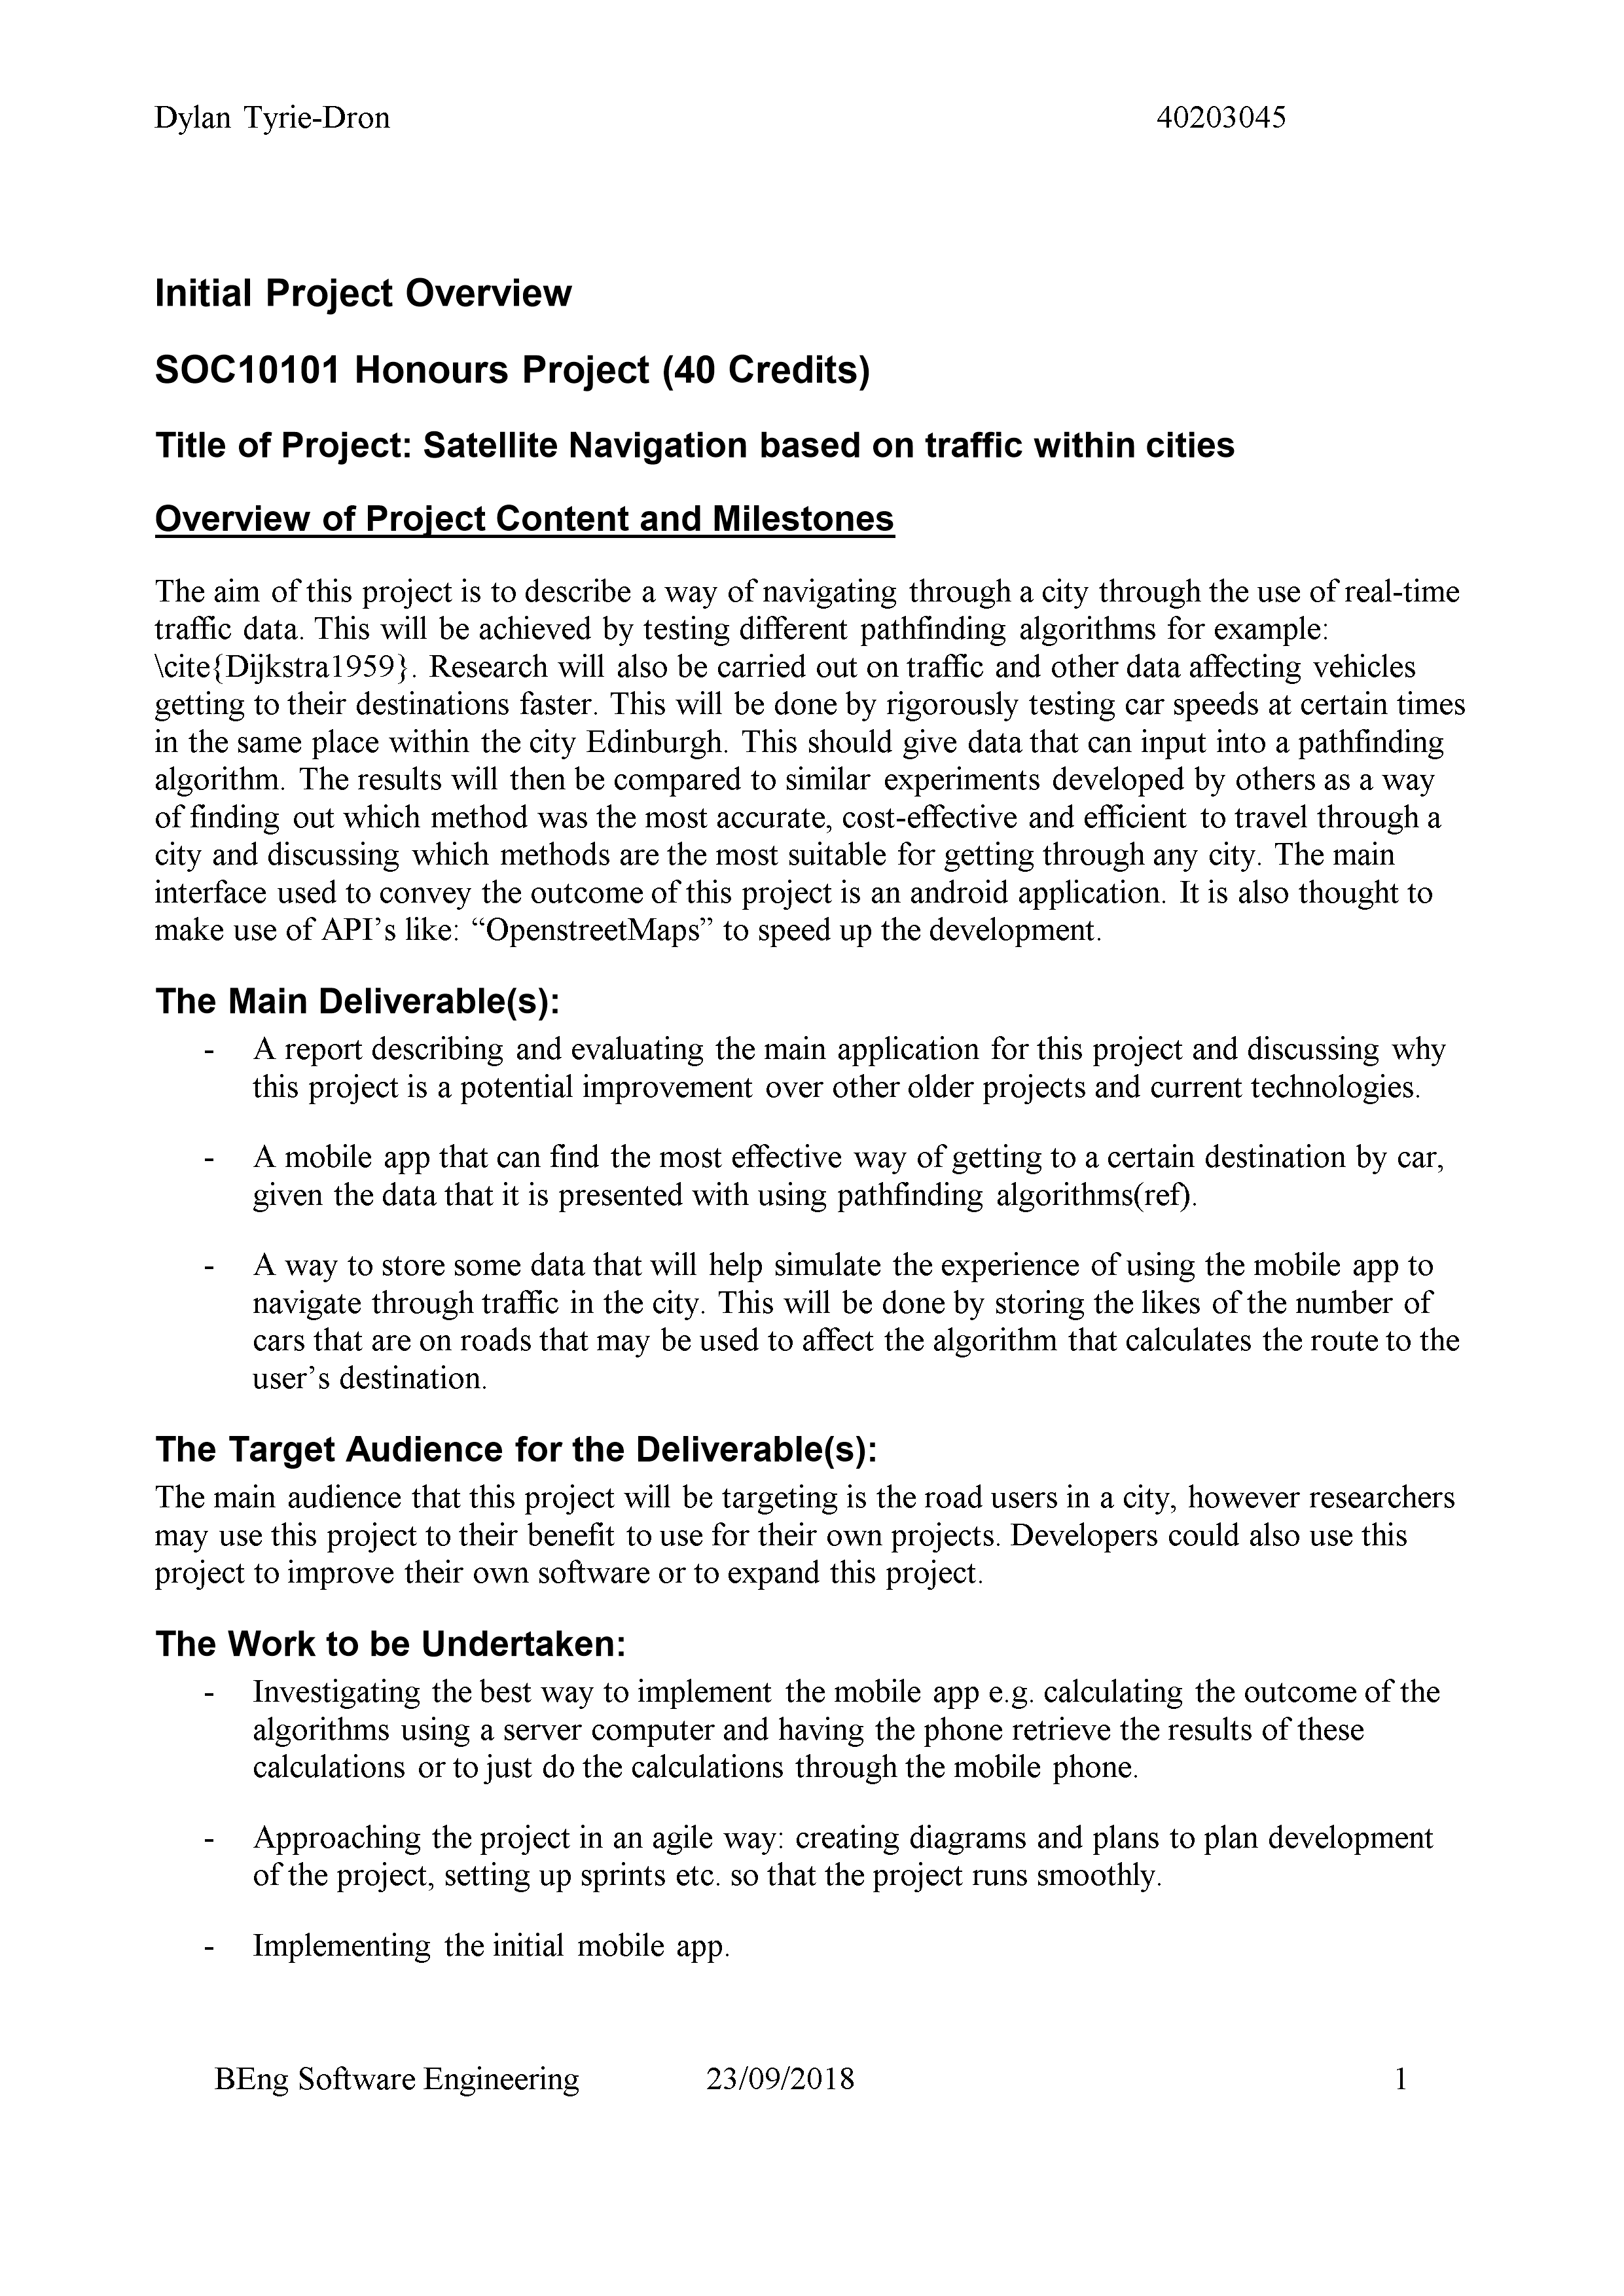
\includegraphics[width=\textwidth,height=\textheight,keepaspectratio]{IPOPage1.png} % fit images to page
\newpage
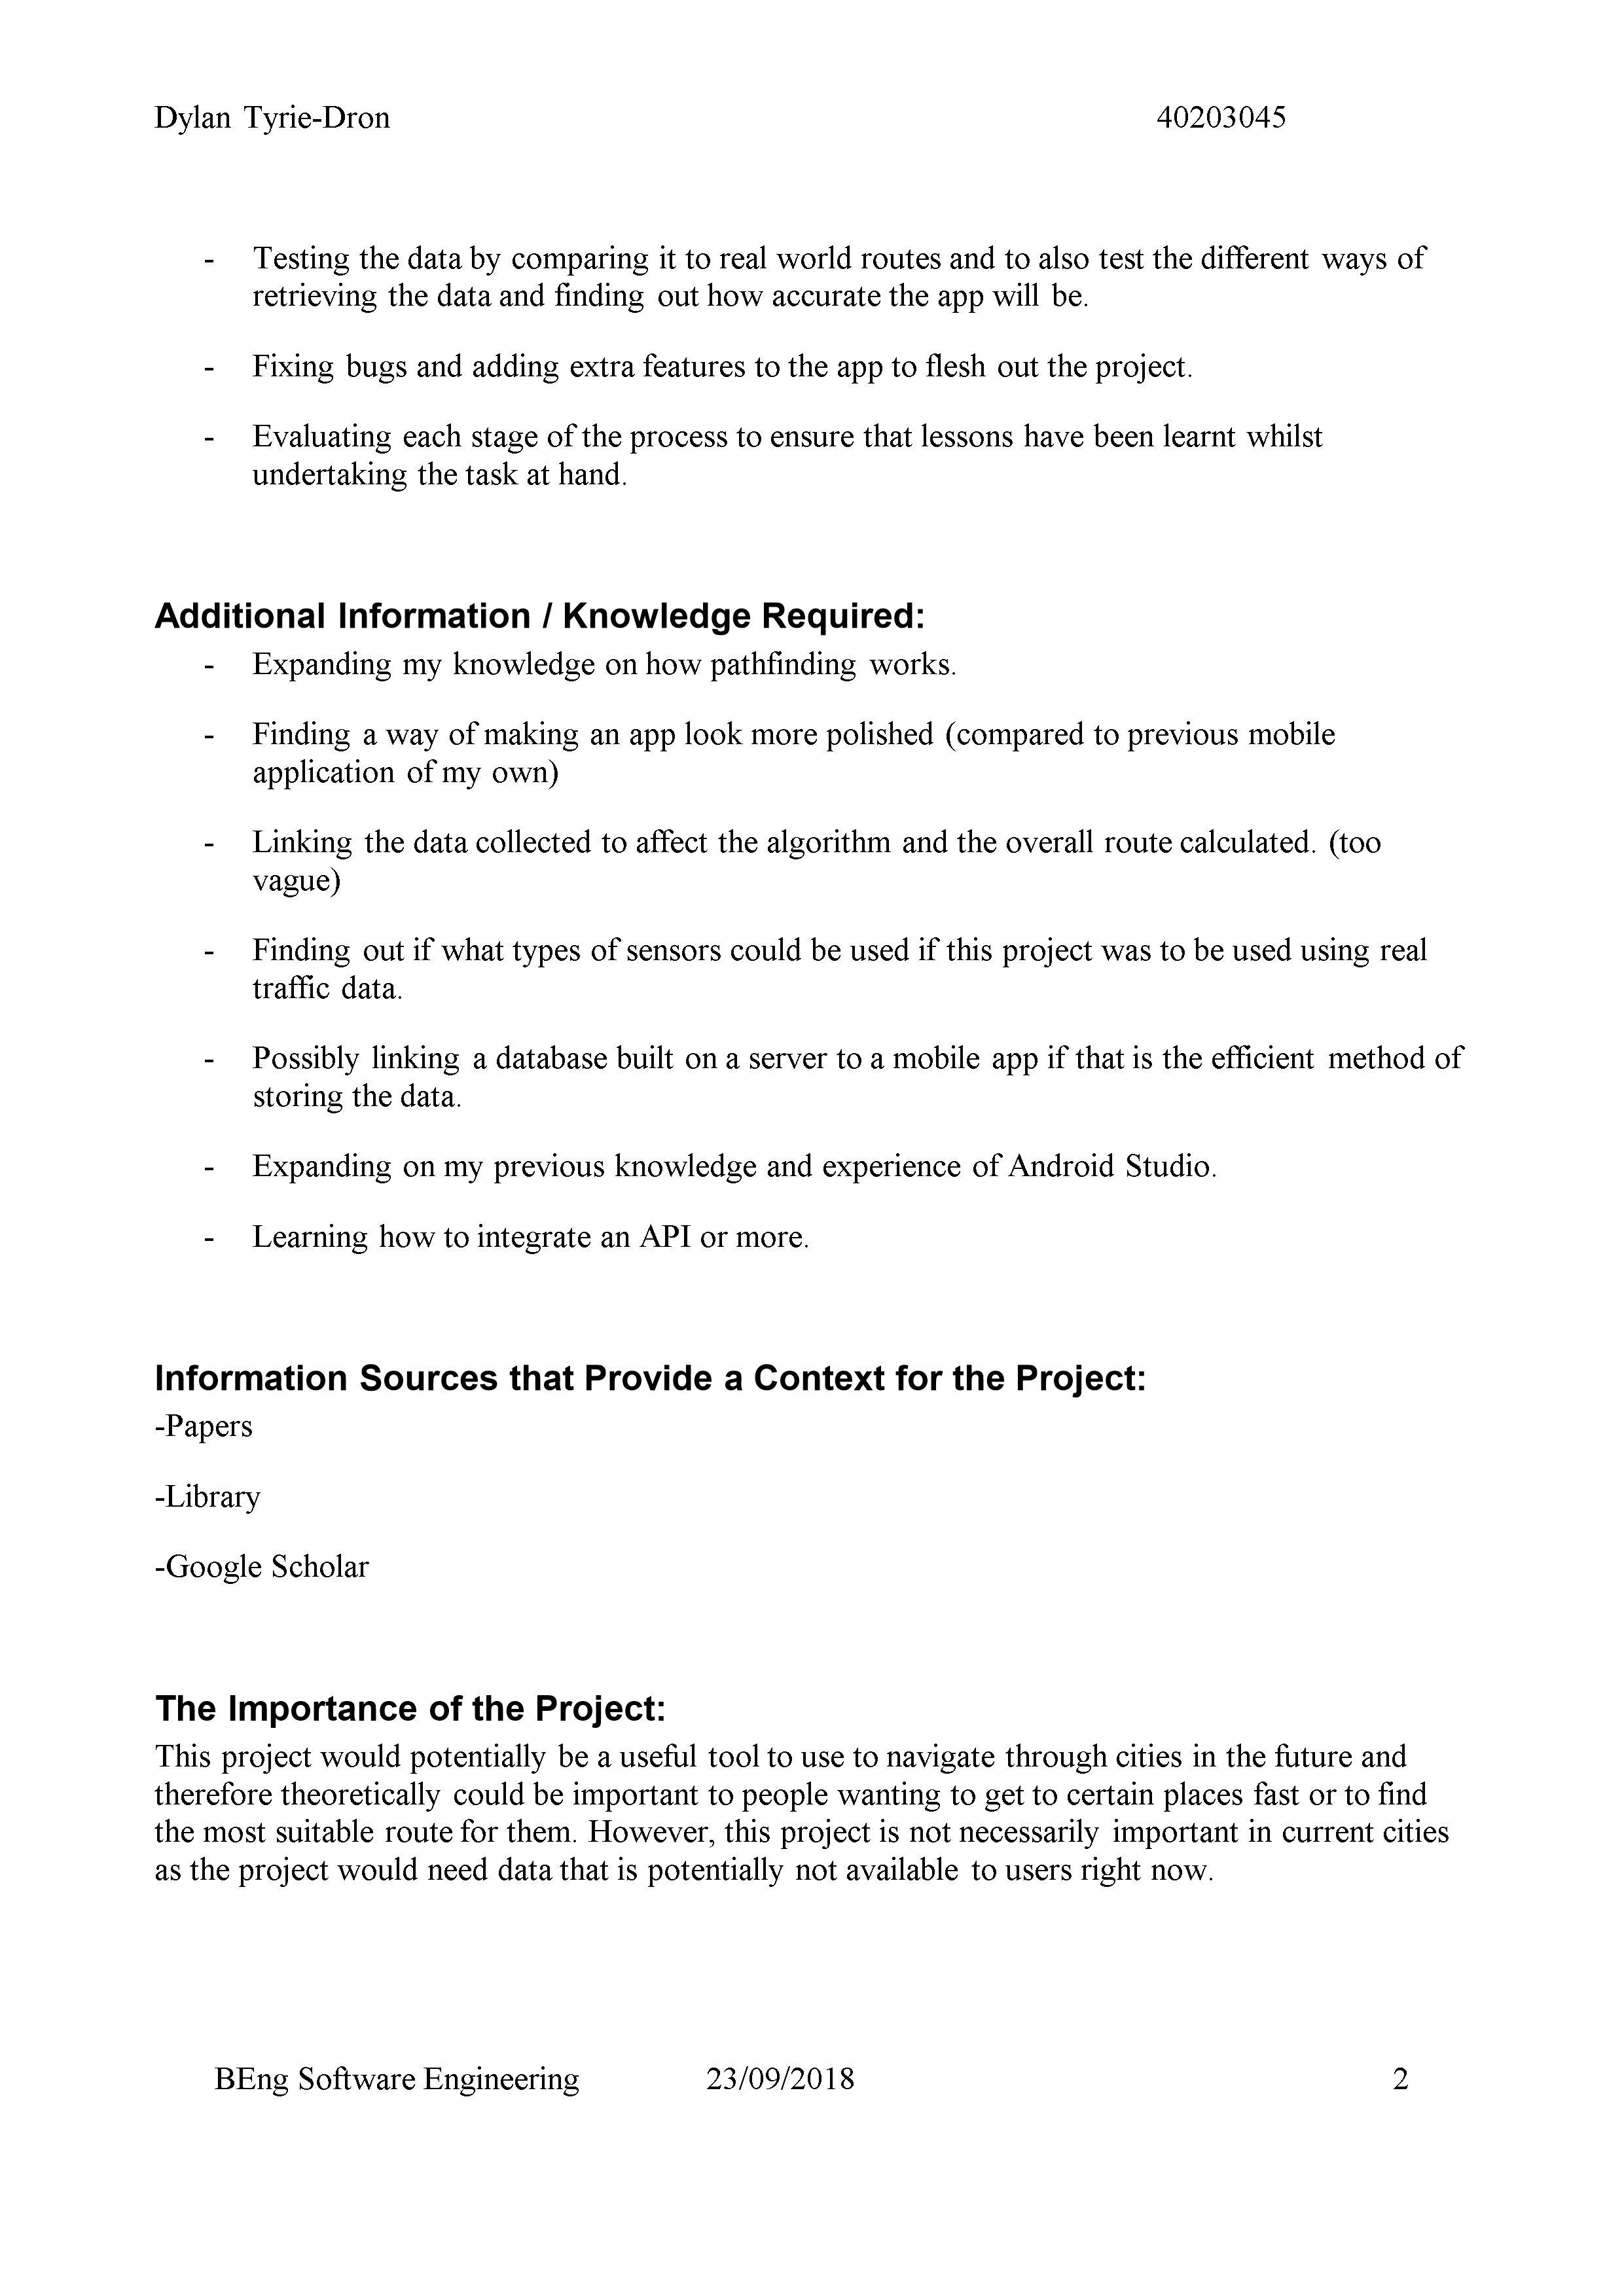
\includegraphics[width=\textwidth,height=\textheight,keepaspectratio]{IPOPage2.png}
\newpage

\includegraphics[width=\textwidth,height=\textheight,keepaspectratio]{IPOPage3.png} 
%insert IPO

% \begin{subappendices}
% \subsection{Example sub appendices}
% ...
% \end{subappendices}

\section{Week 9 interim report}
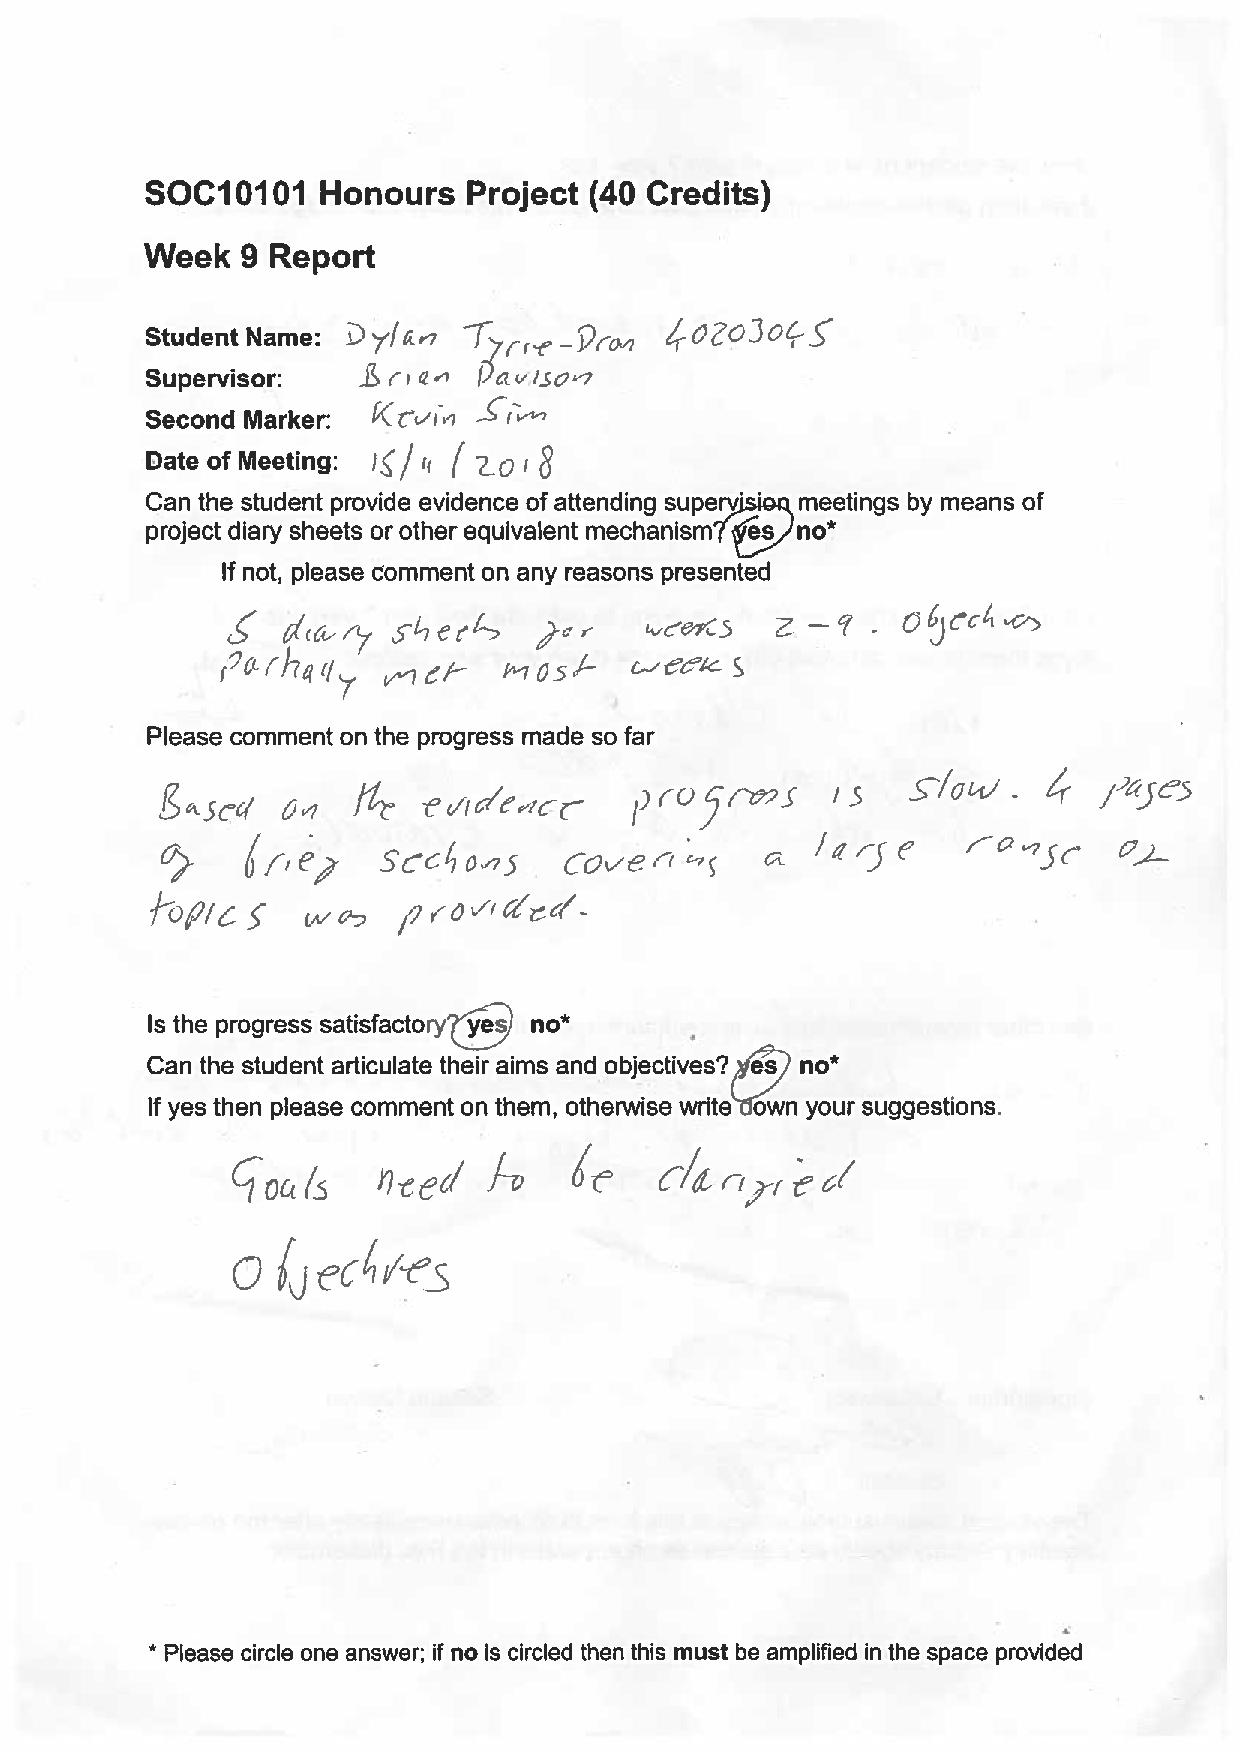
\includegraphics[width=\textwidth,height=\textheight,keepaspectratio]{./appendicies/40203045_interim-1.pdf}
\newpage
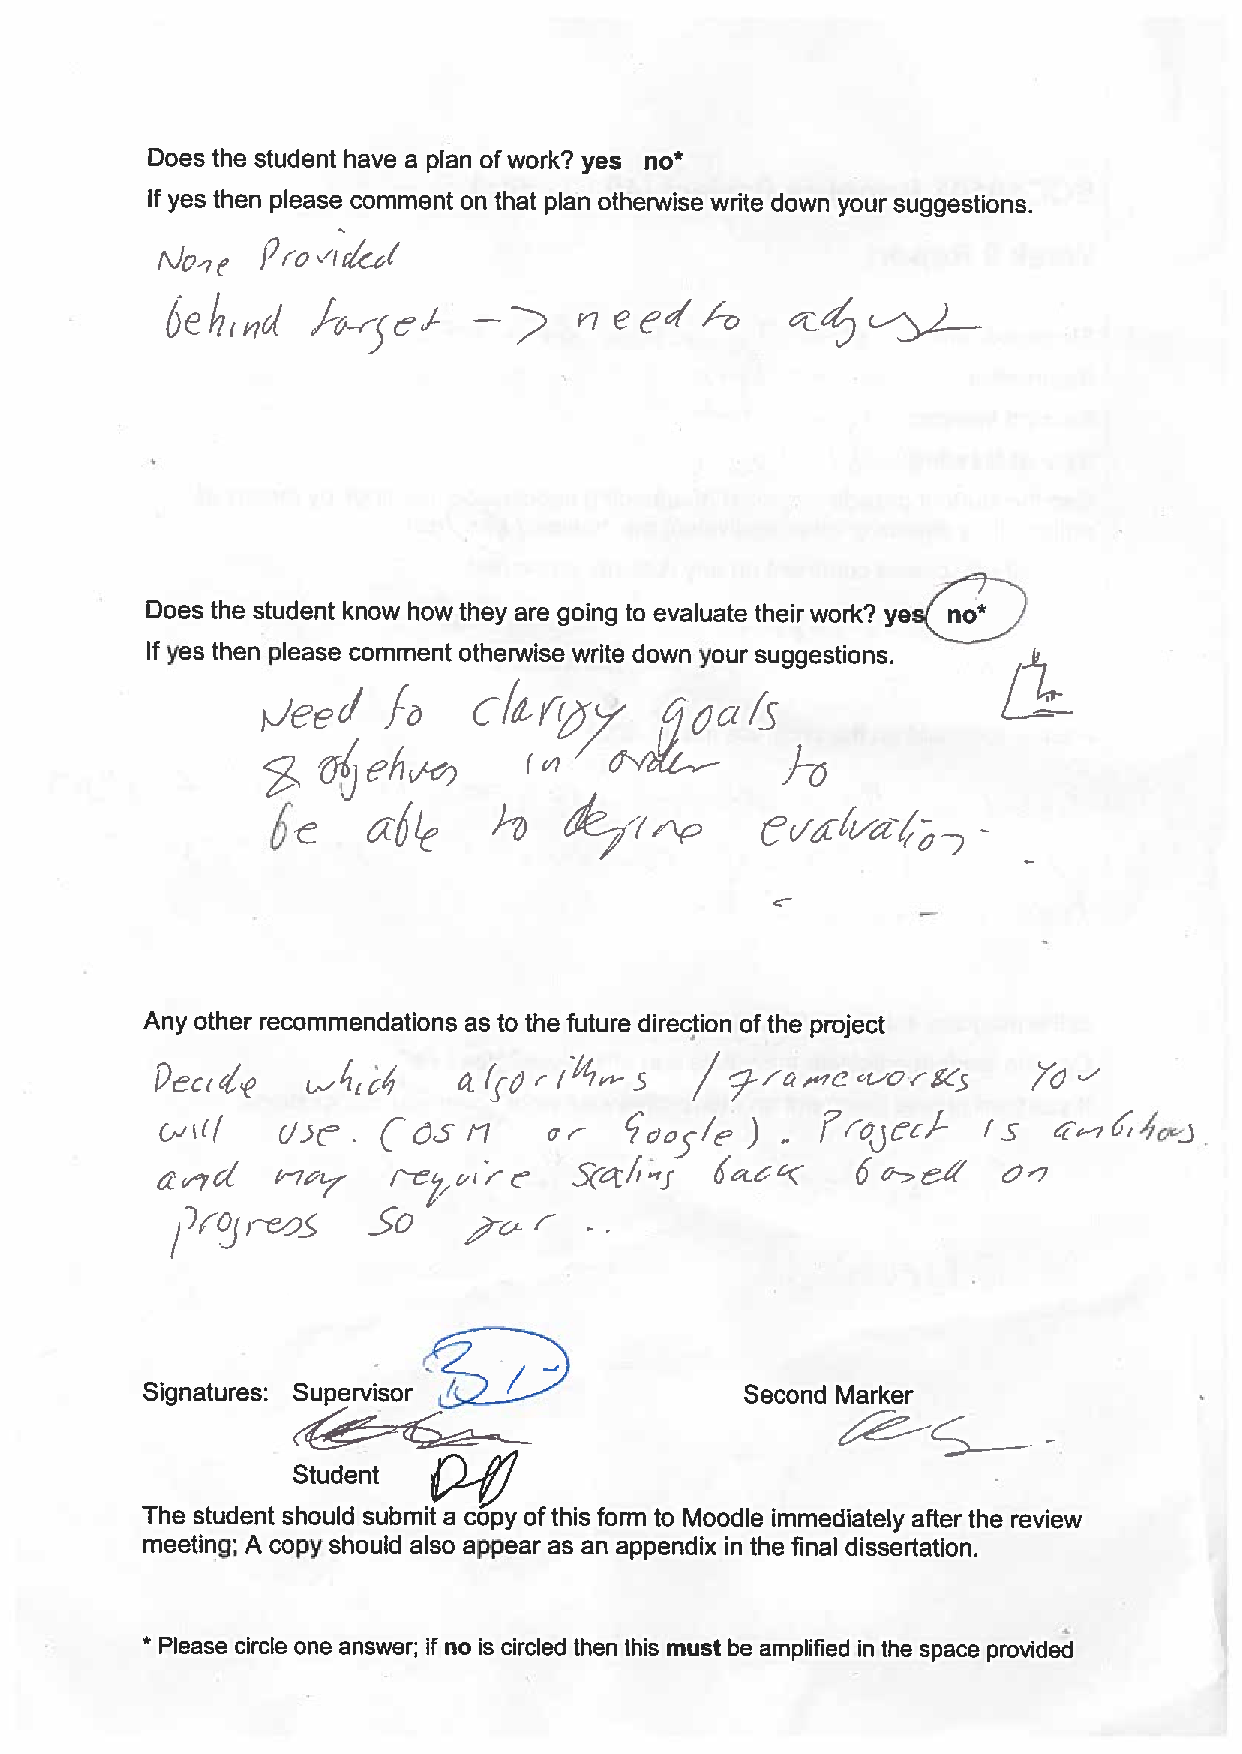
\includegraphics[width=\textwidth,height=\textheight,keepaspectratio]{./appendicies/40203045_interim-2.pdf}

 \section{Diary Sheets (or other project management evidence)}
% Insert diary sheets here together with any project management plan you have
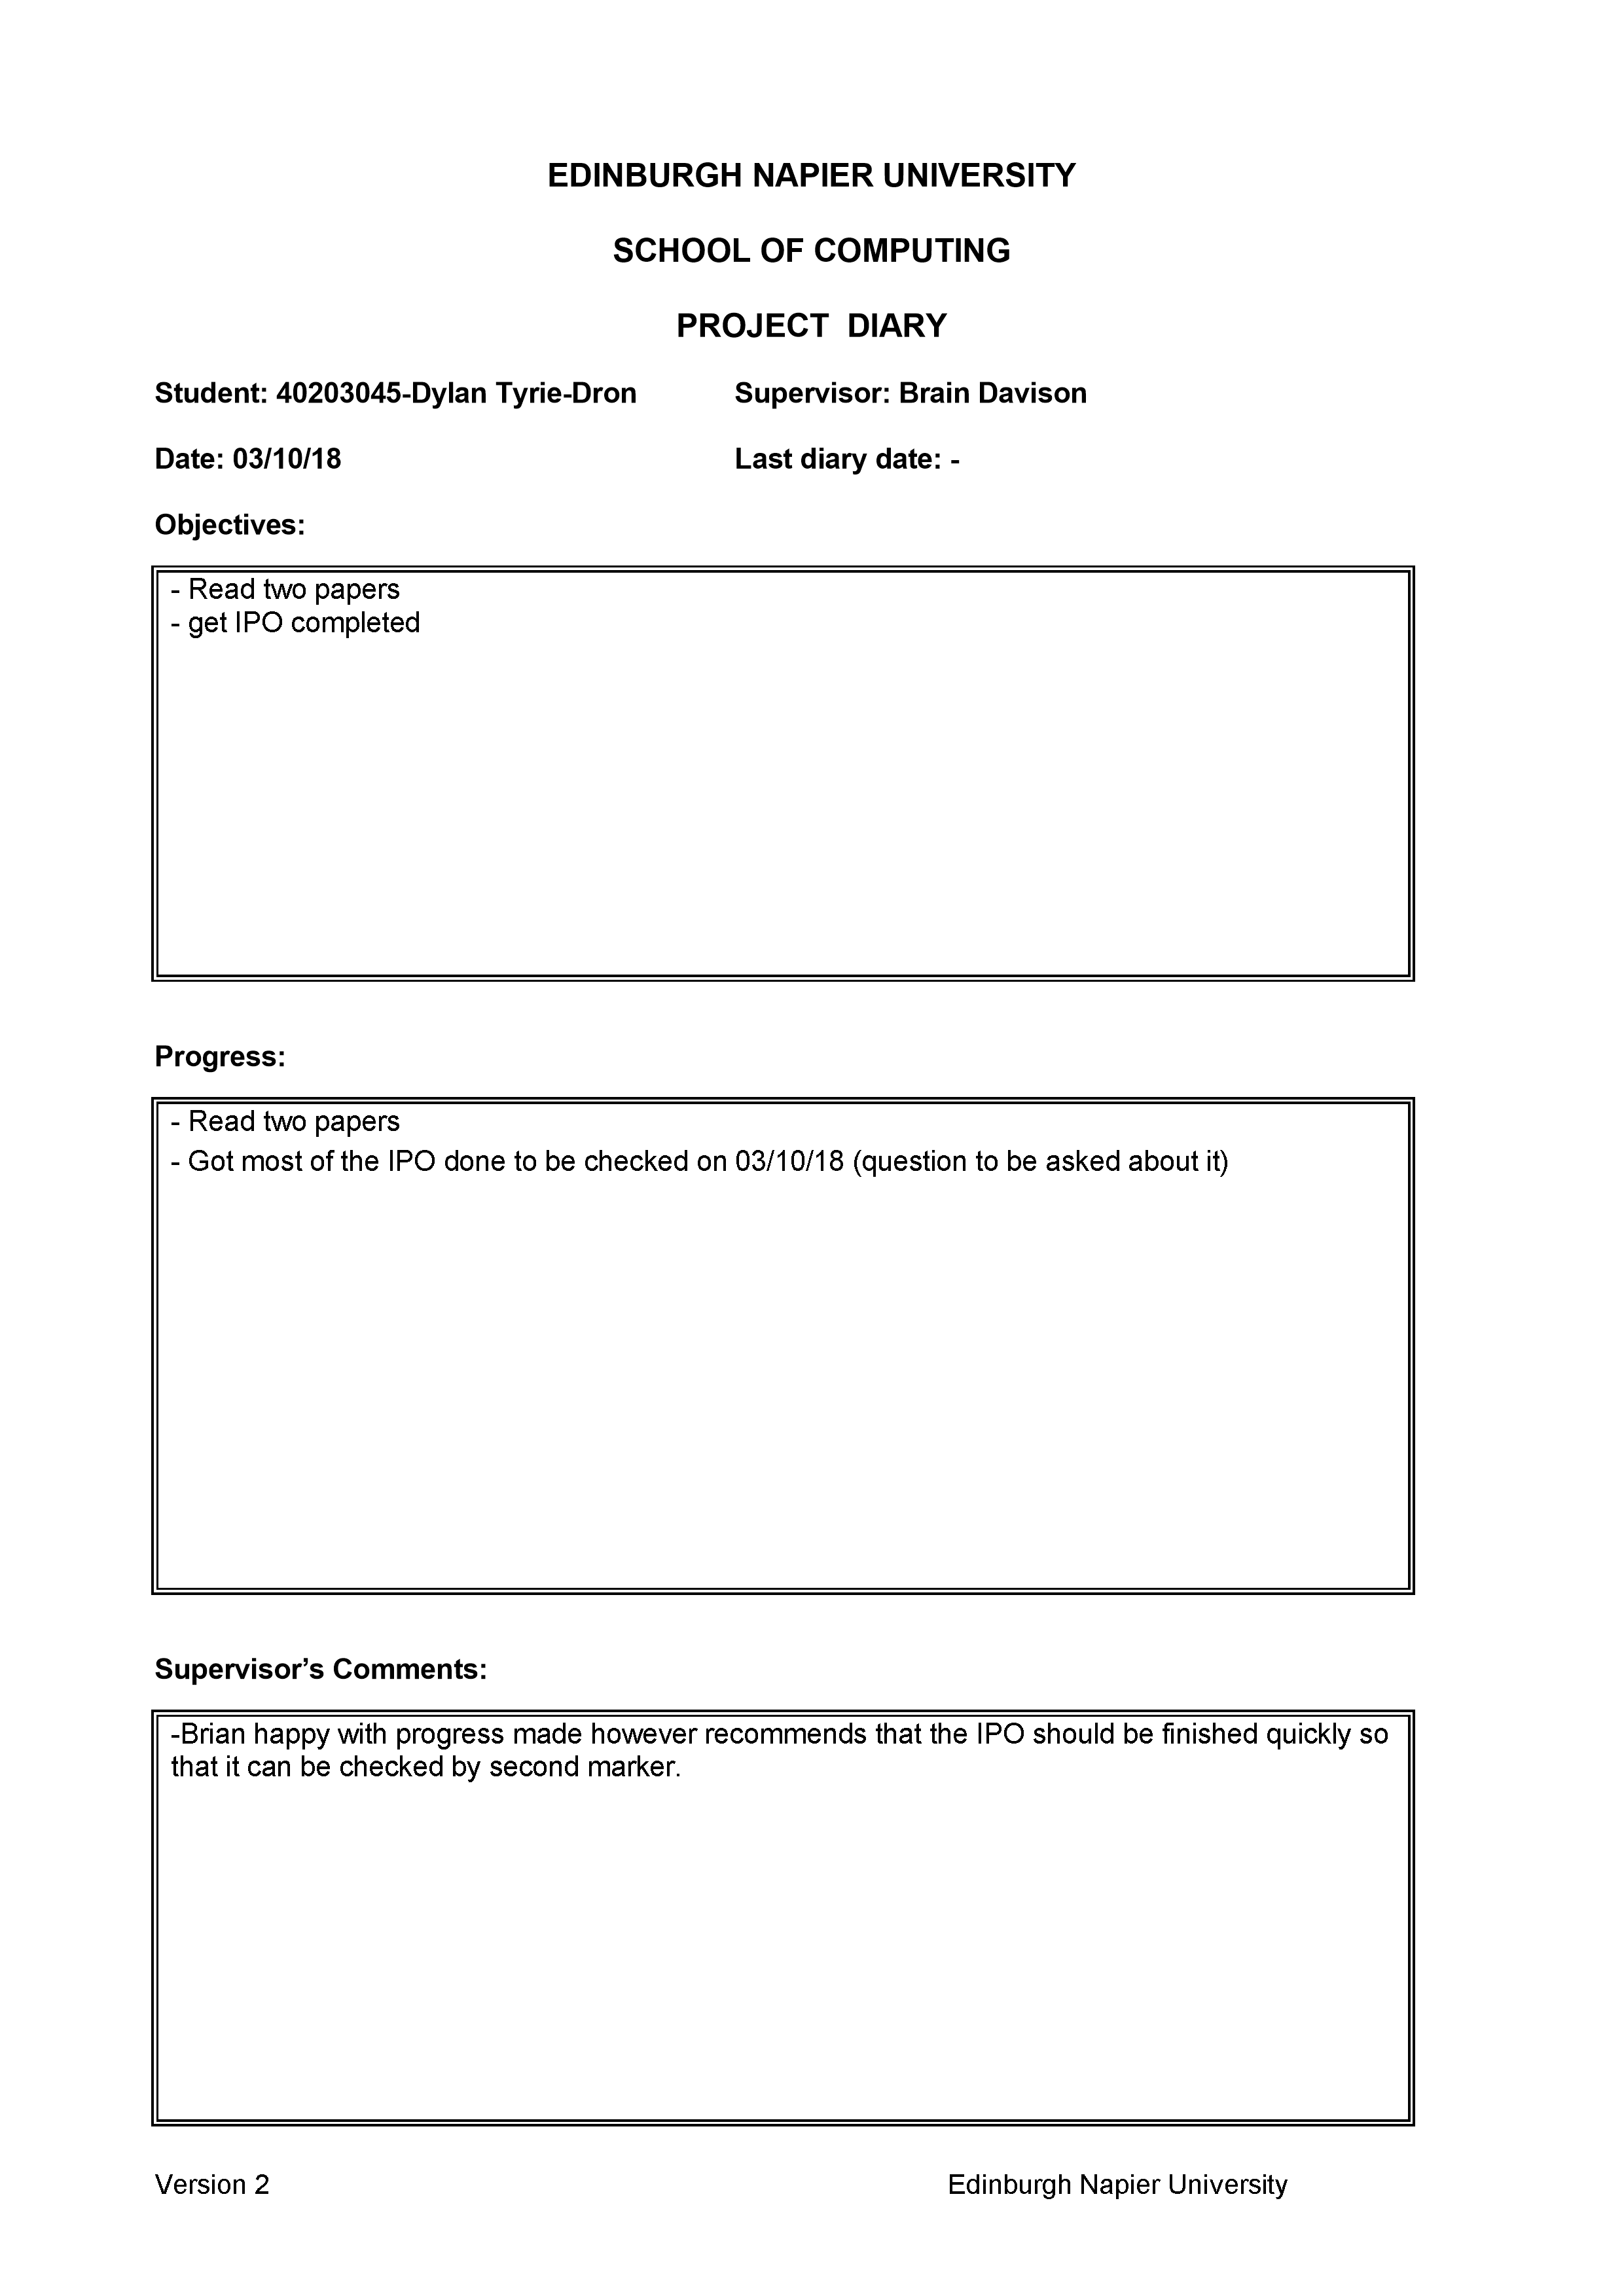
\includegraphics[width=\textwidth,height=\textheight,keepaspectratio]{diary1.png} % fit images to page
\newpage
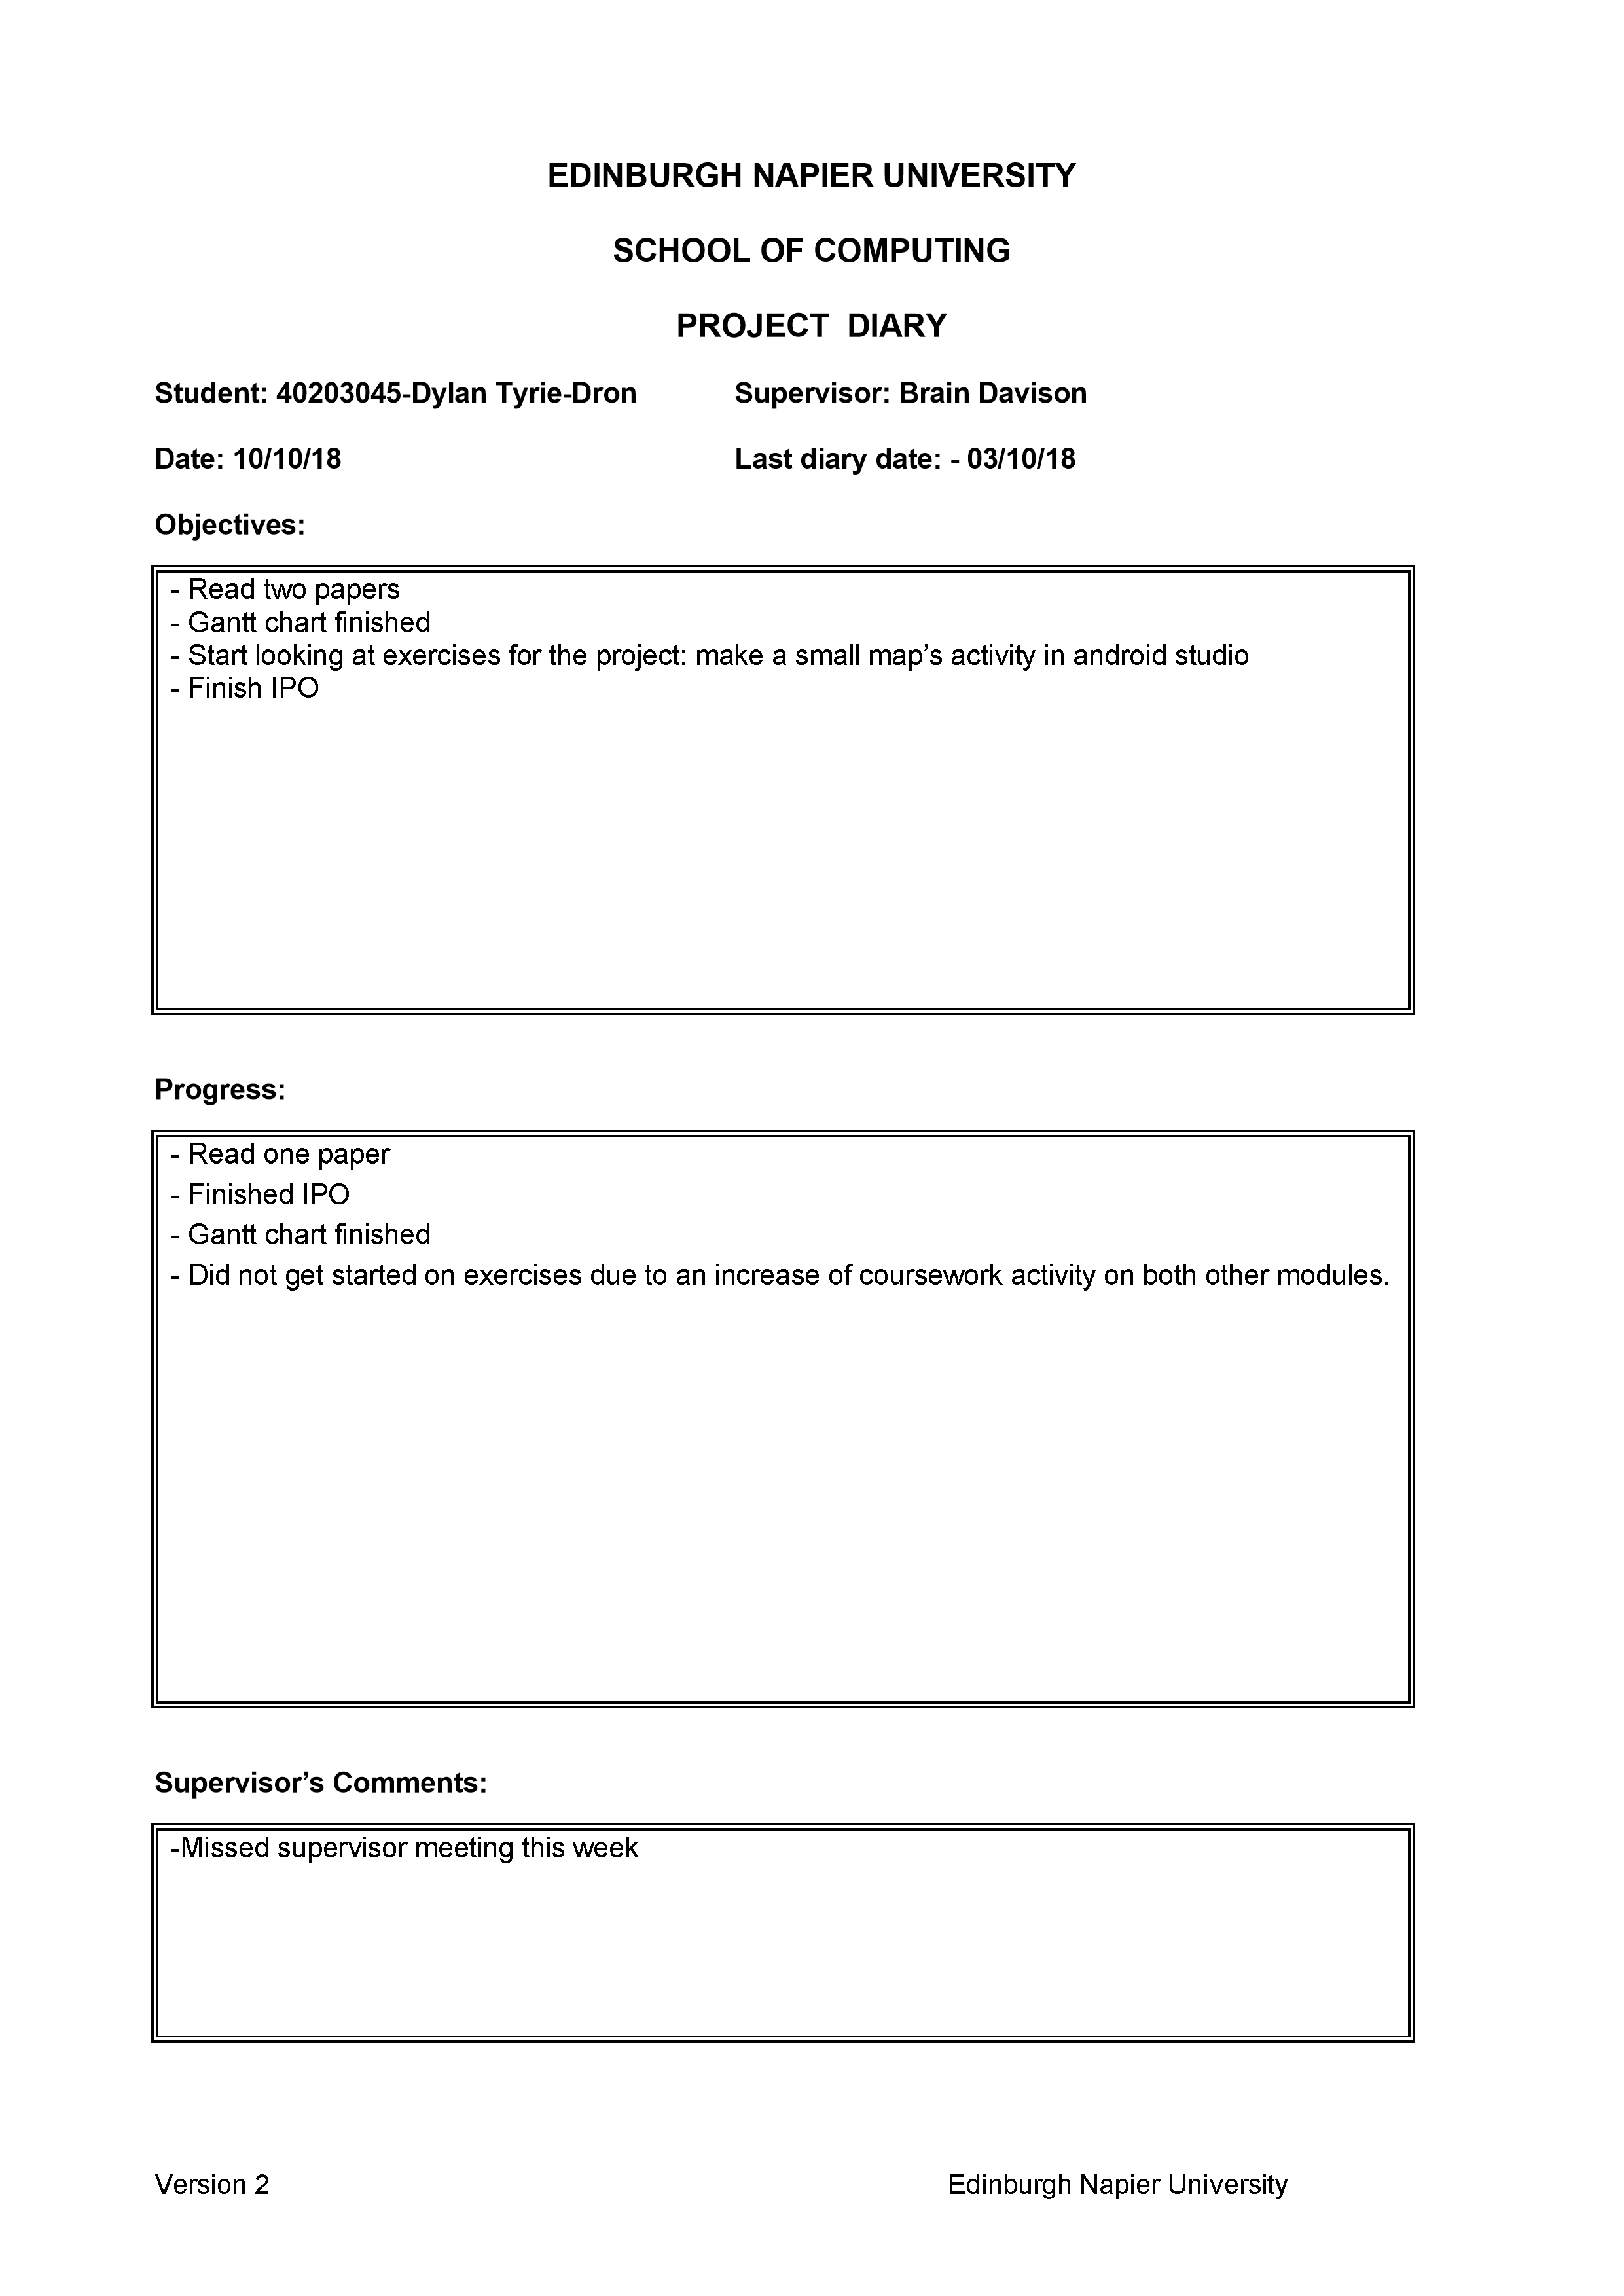
\includegraphics[width=\textwidth,height=\textheight,keepaspectratio]{diary2.png}
\newpage
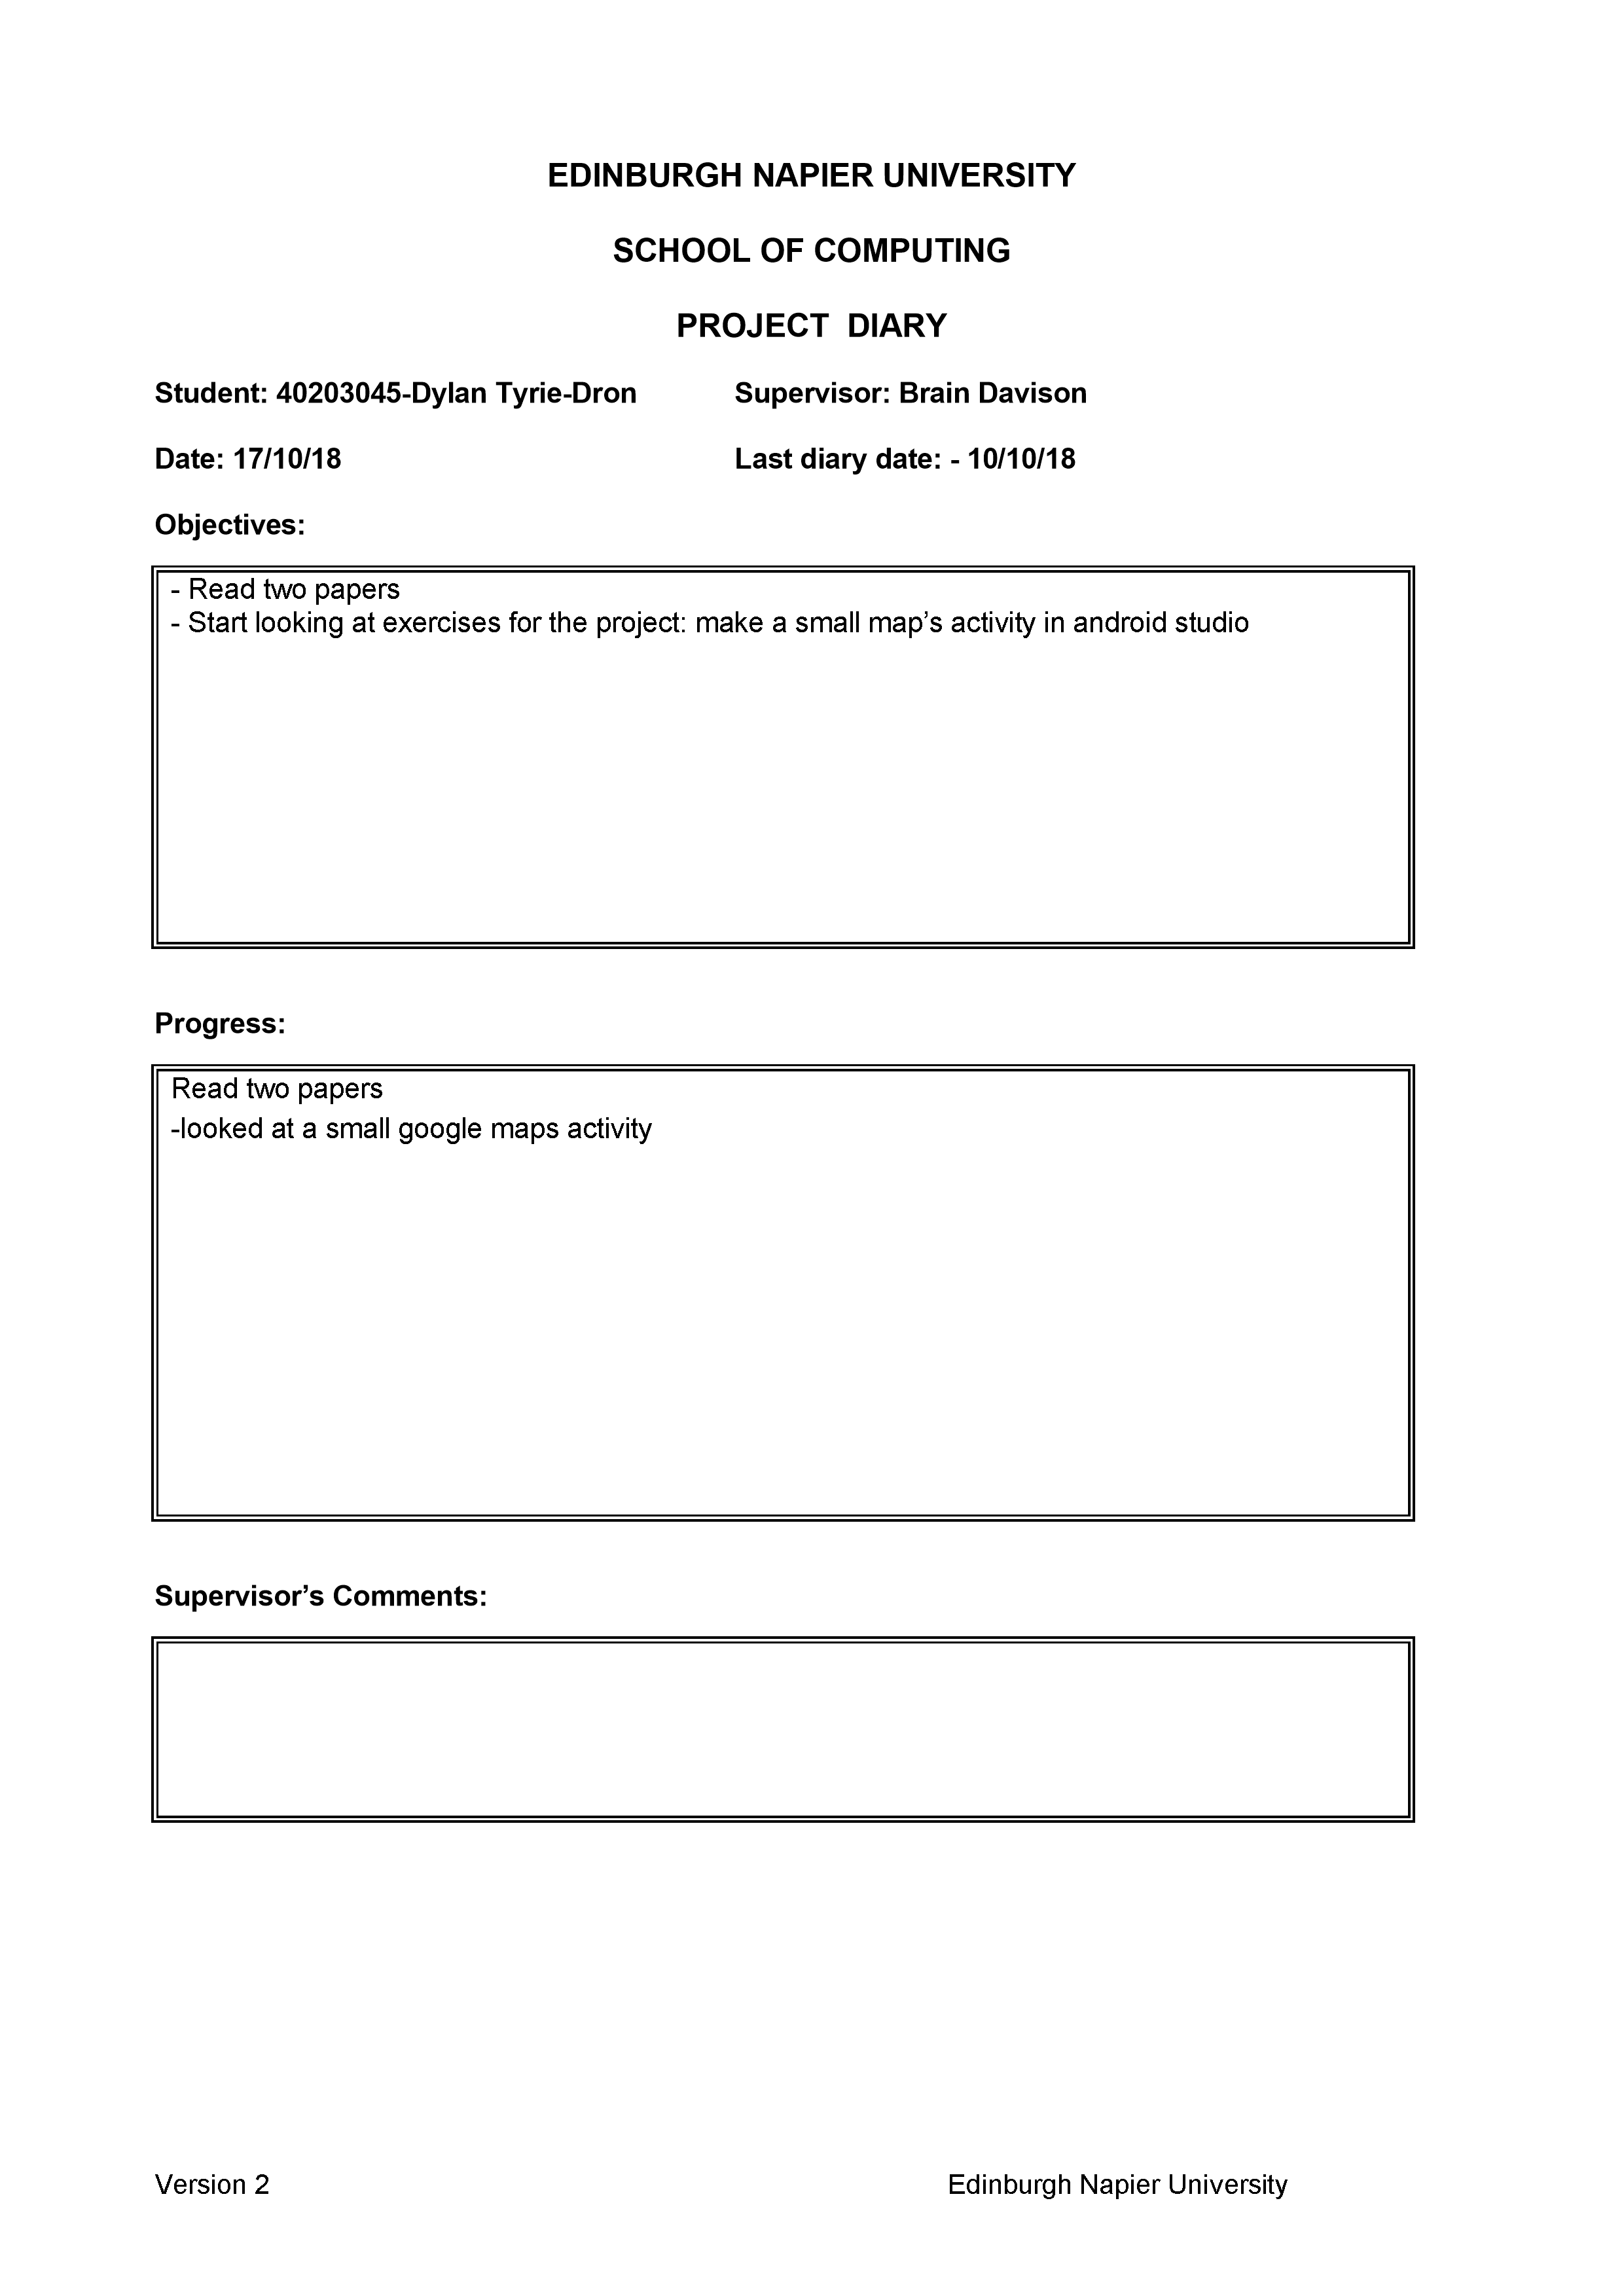
\includegraphics[width=\textwidth,height=\textheight,keepaspectratio]{diary3.png} 
\newpage
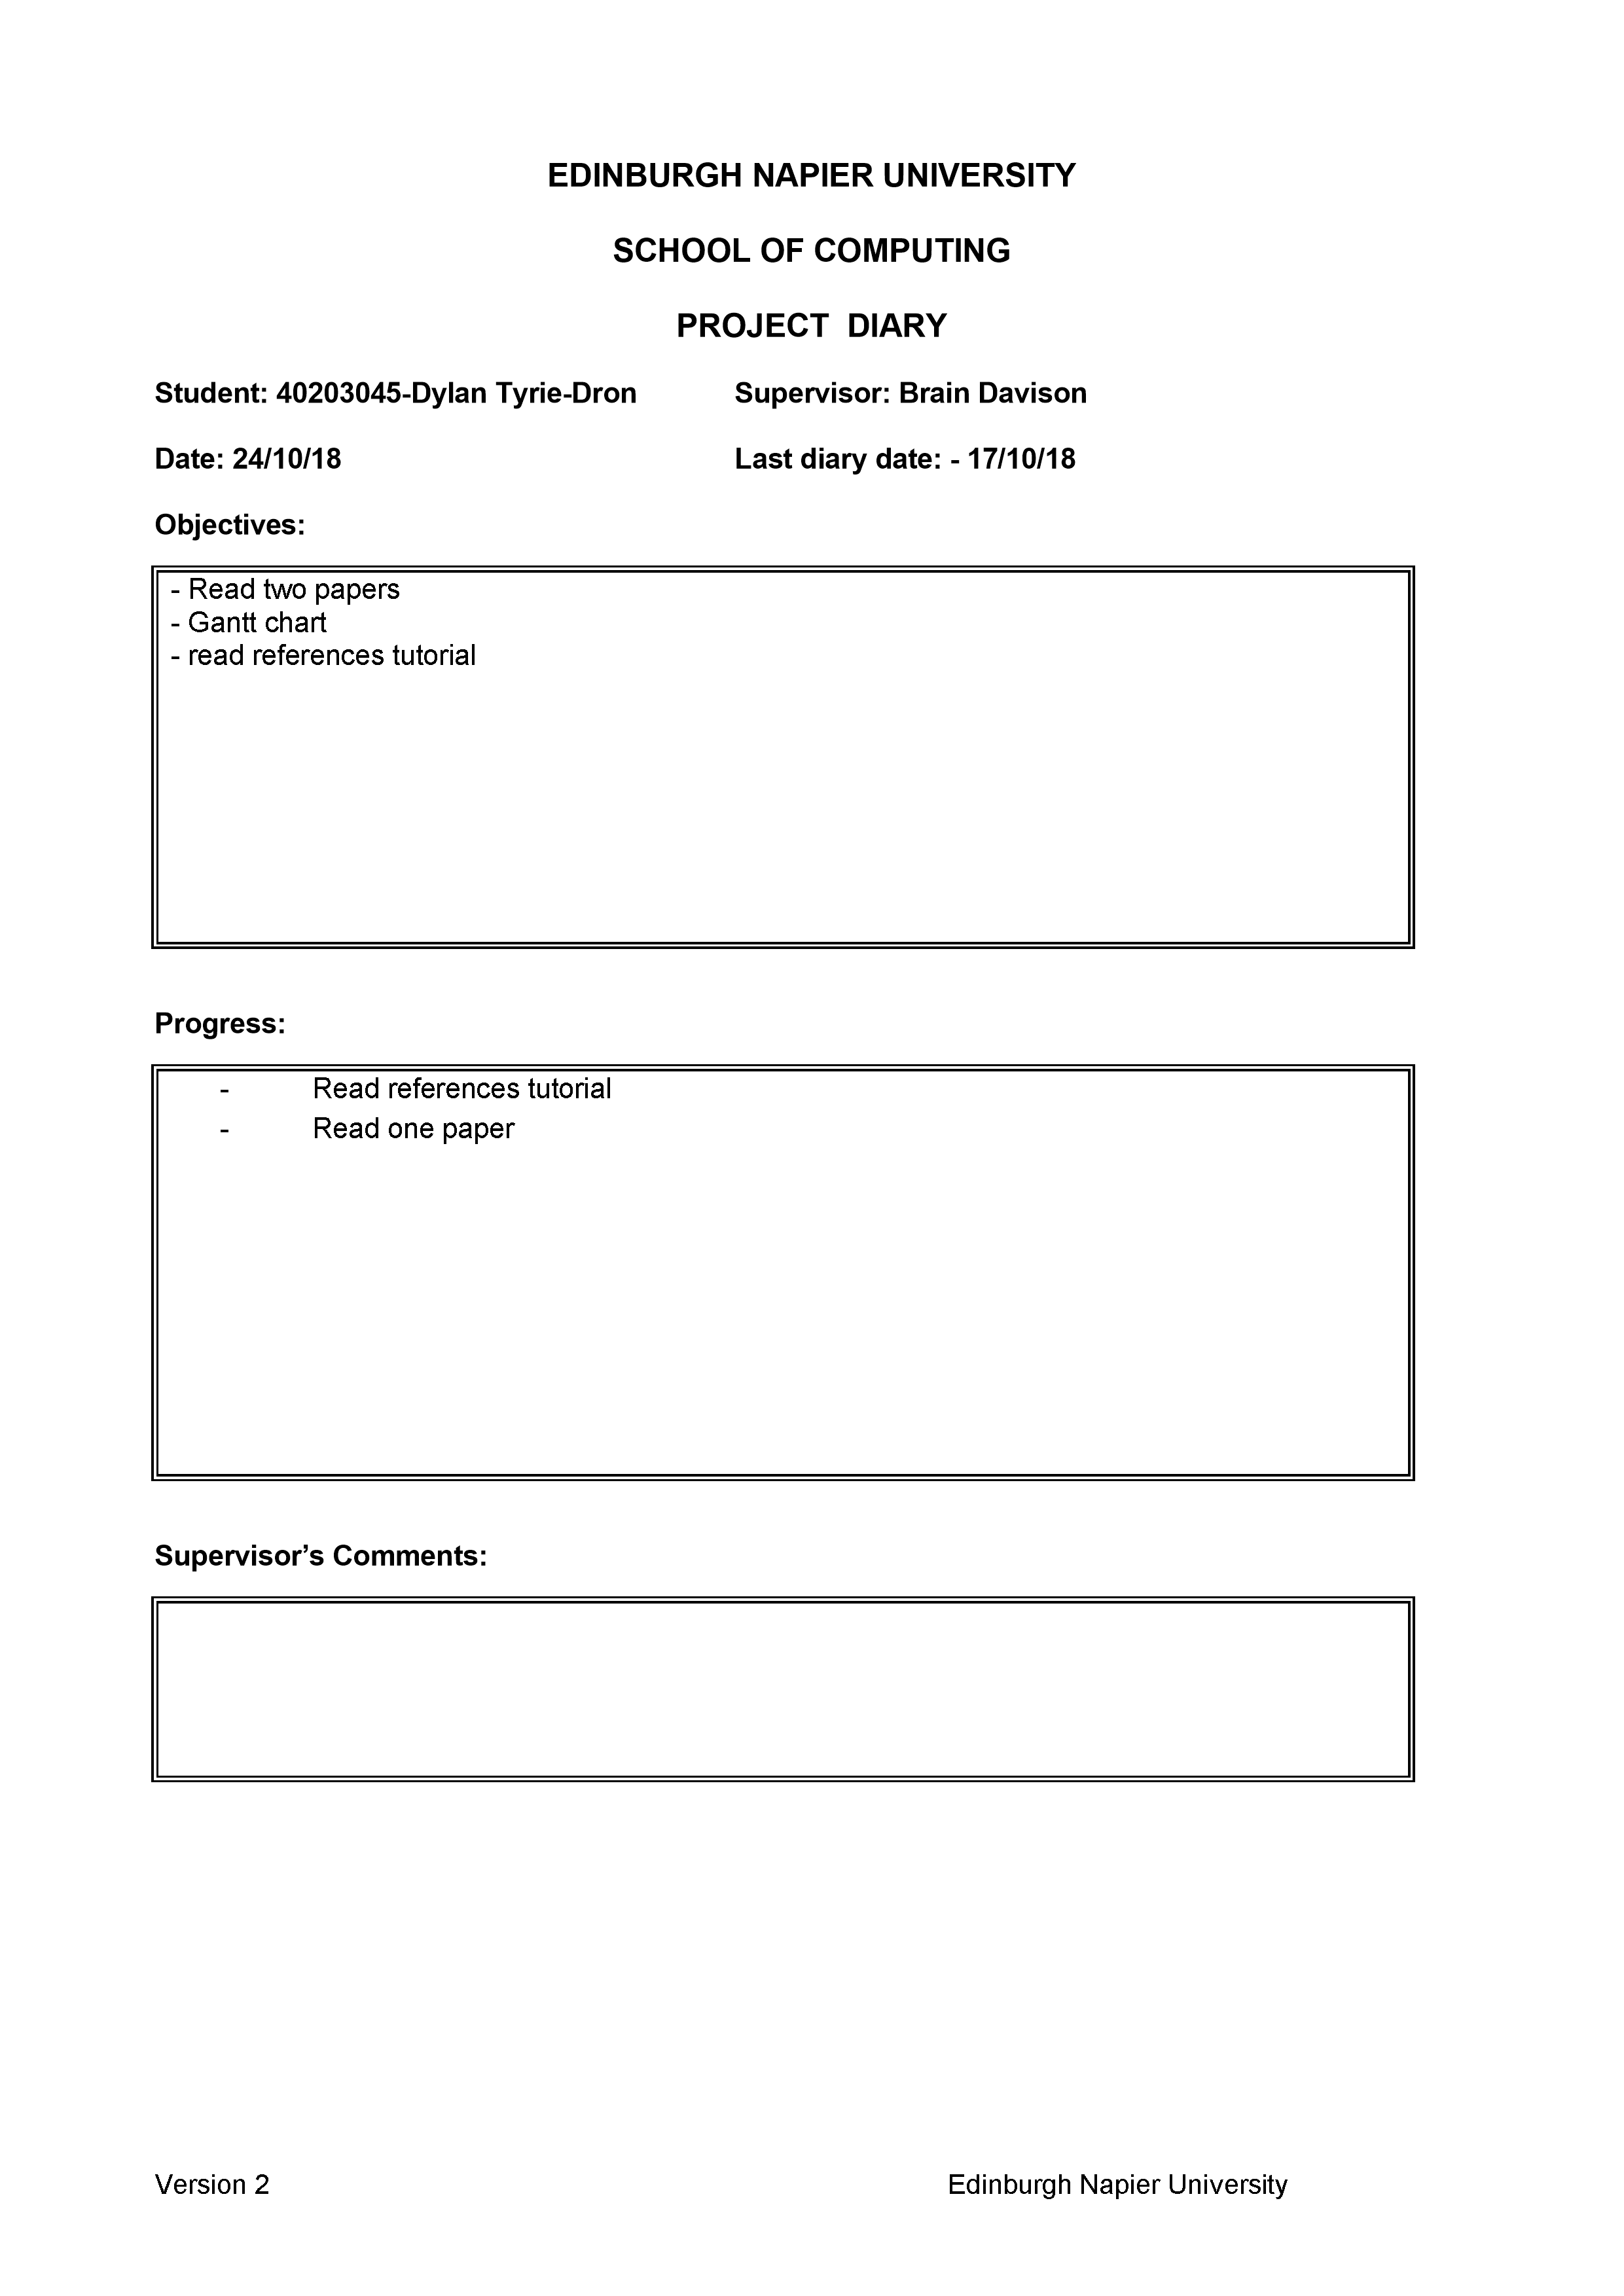
\includegraphics[width=\textwidth,height=\textheight,keepaspectratio]{diary4.png} 
\newpage
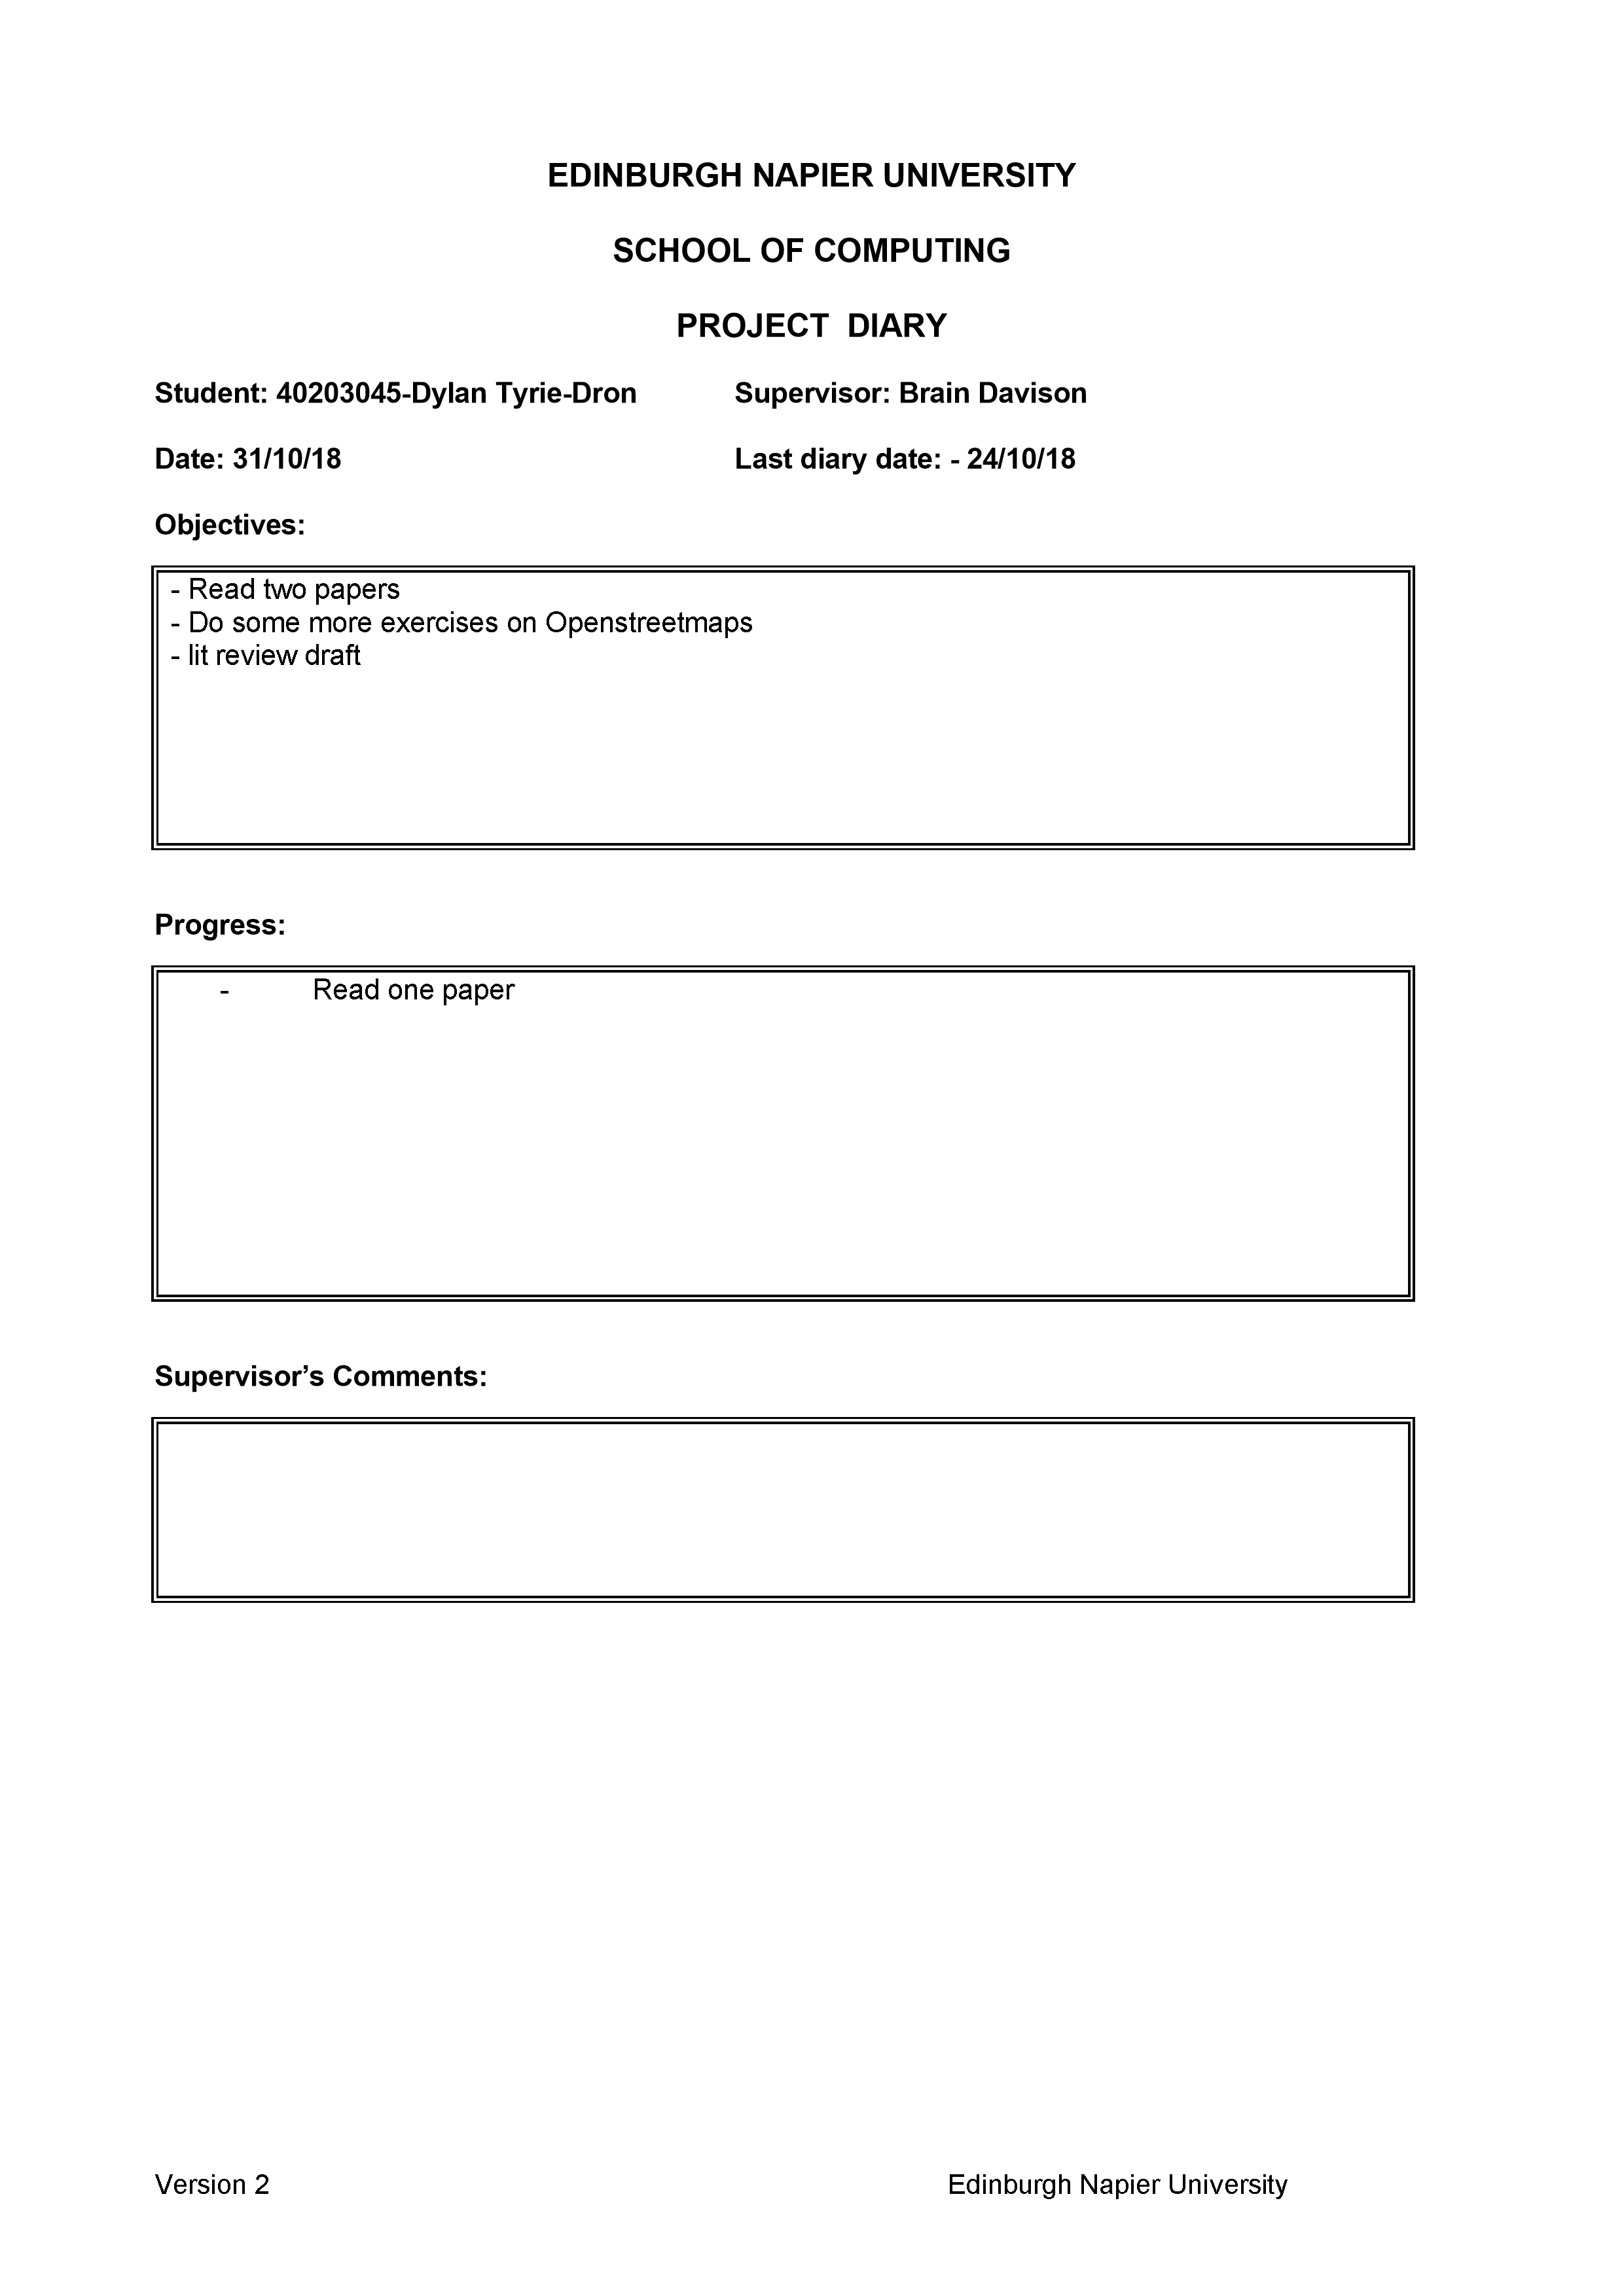
\includegraphics[width=\textwidth,height=\textheight,keepaspectratio]{diary5.png}
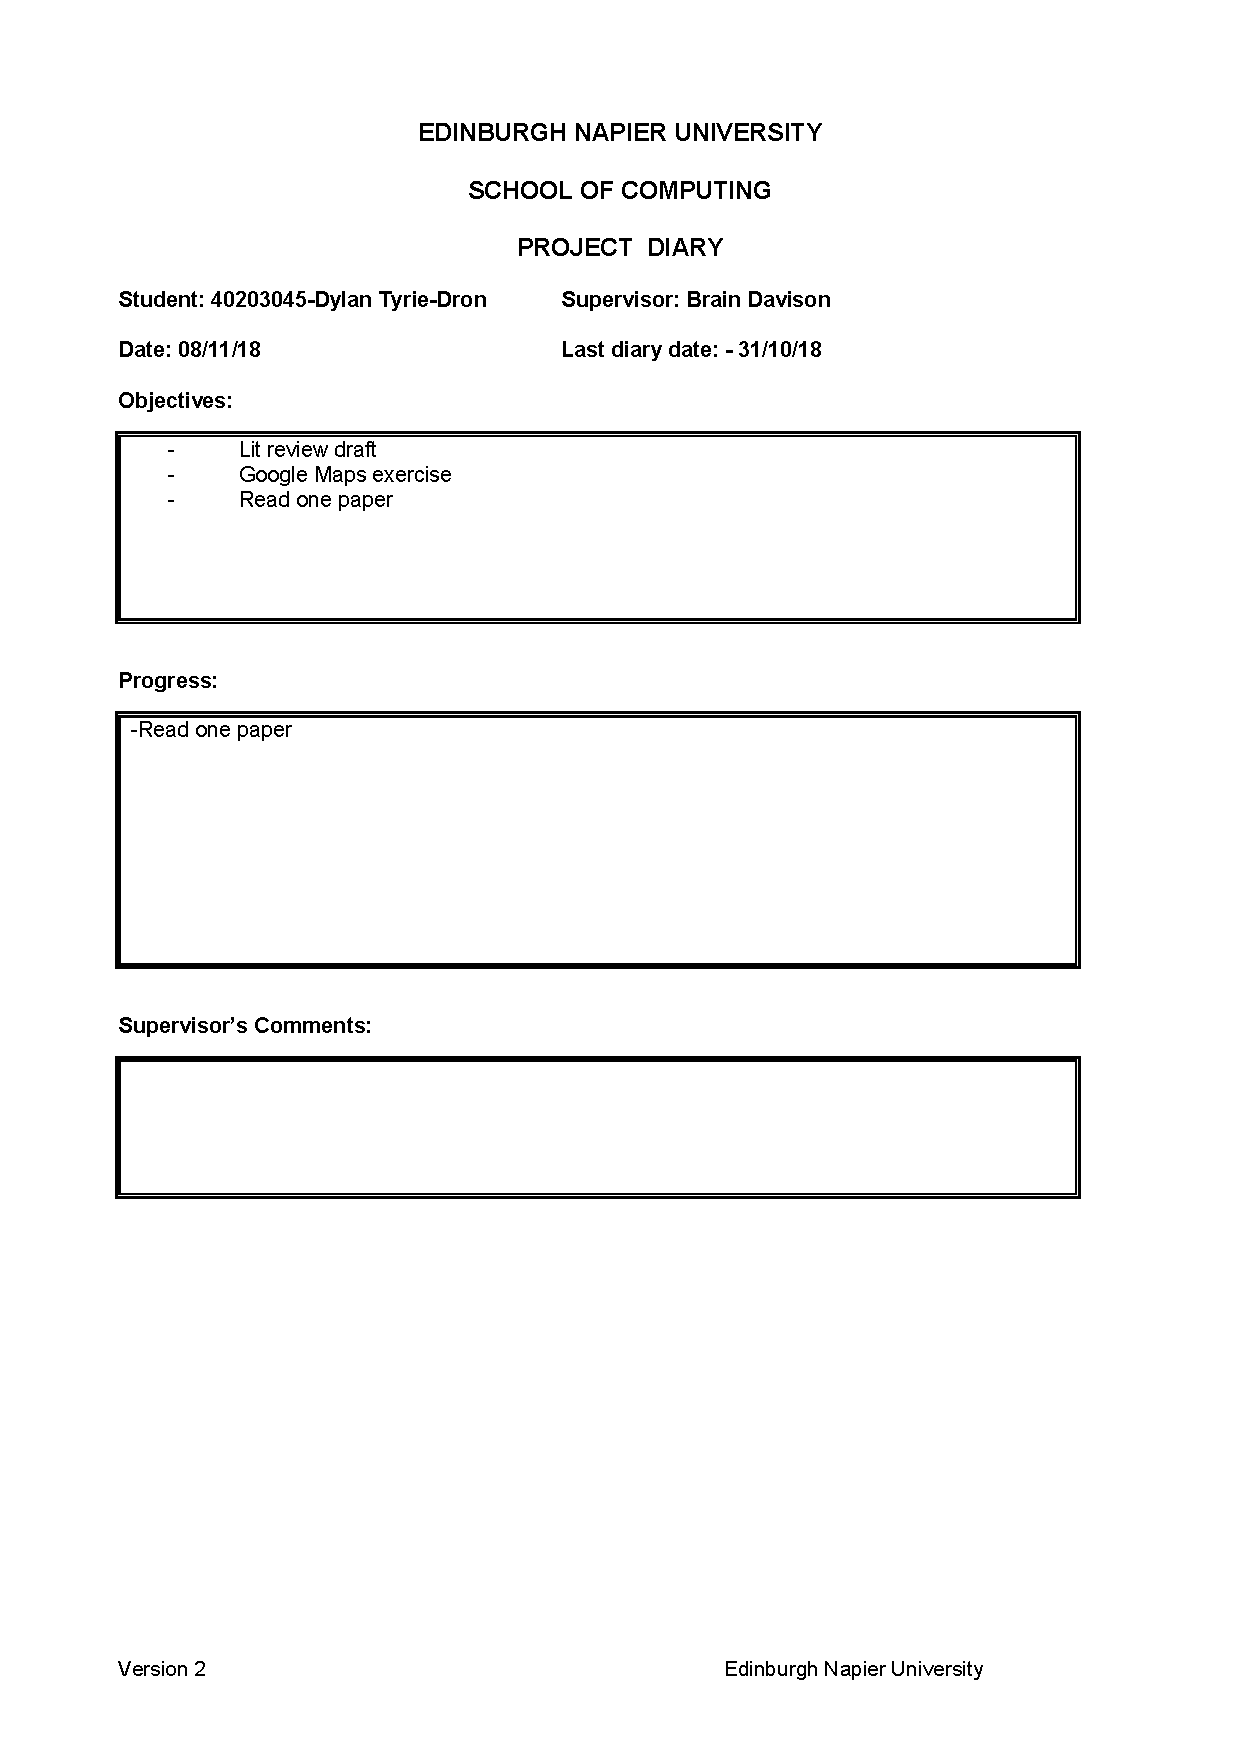
\includegraphics[width=\textwidth,height=\textheight,keepaspectratio]{project_diary_6th_entry.pdf}
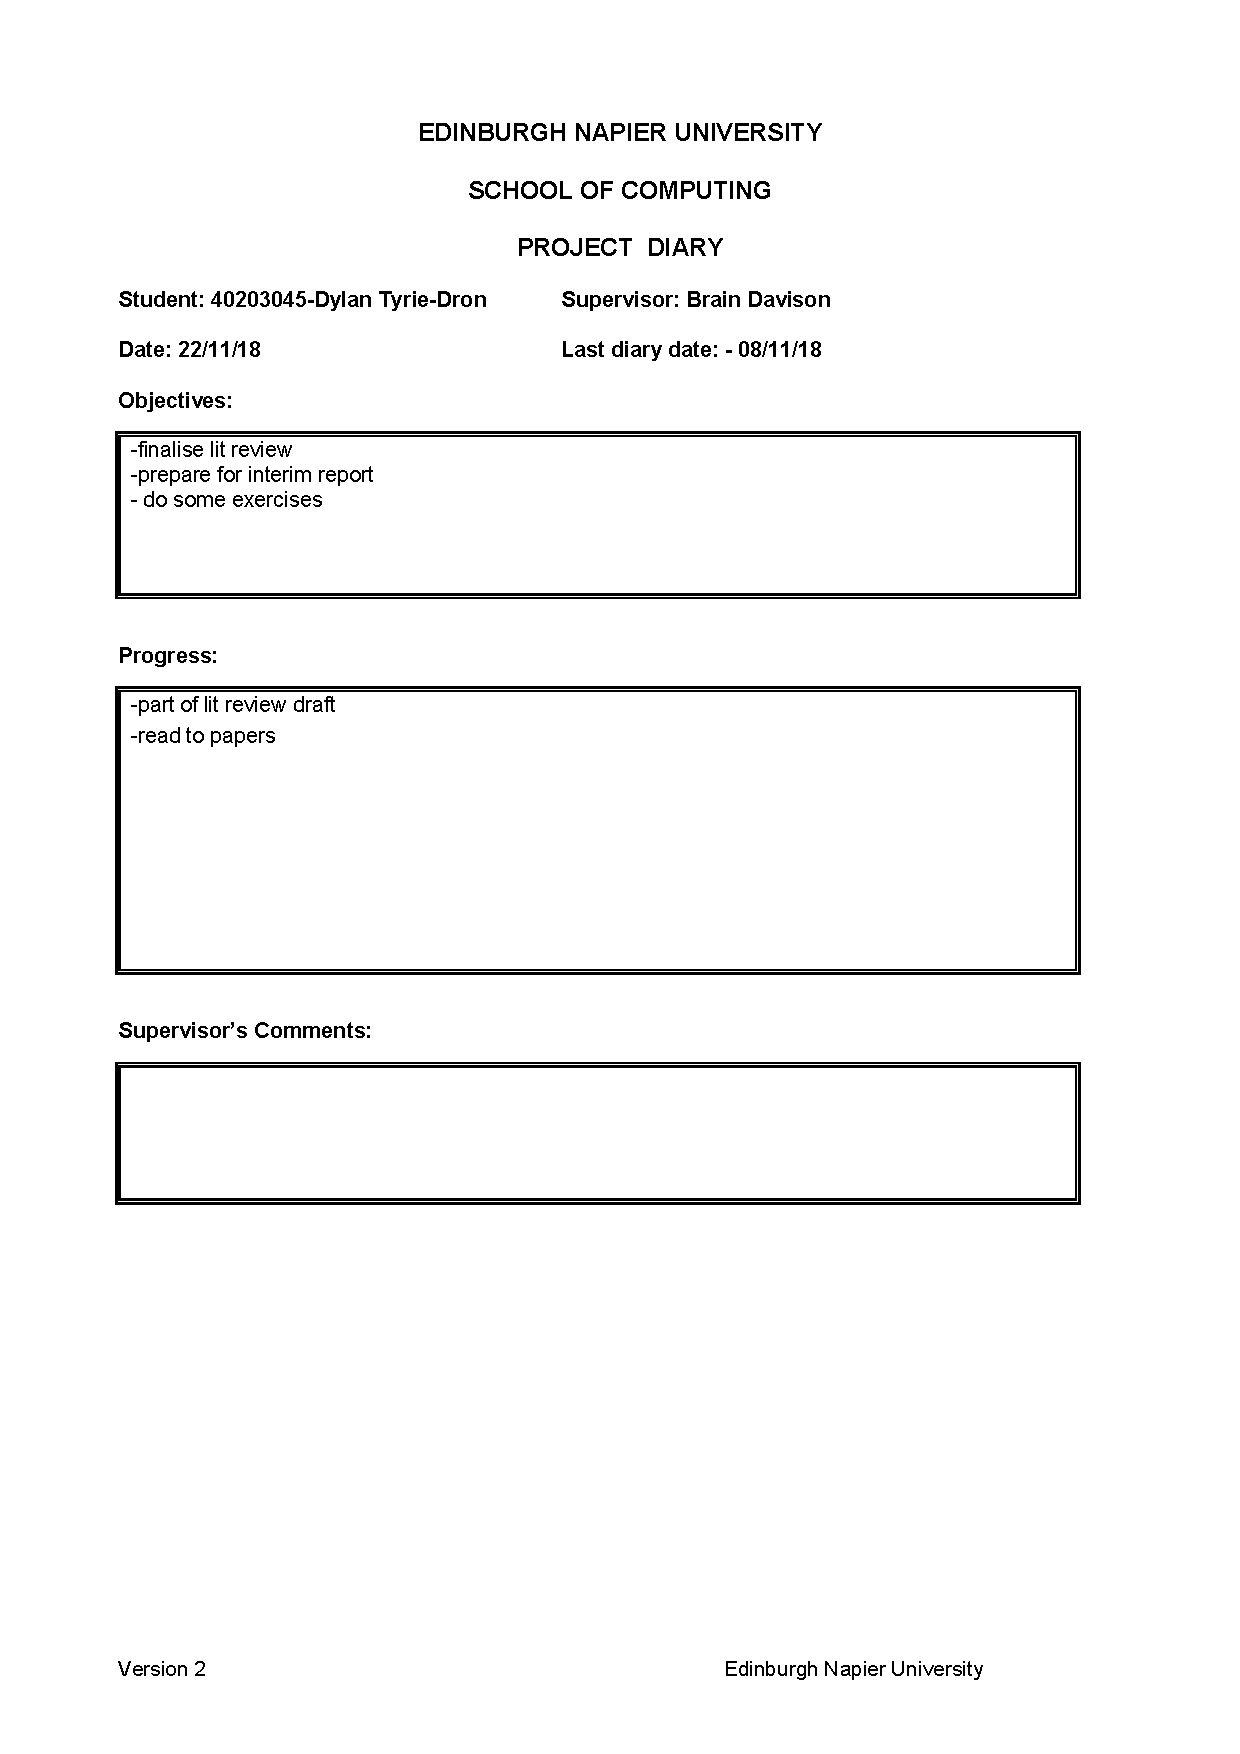
\includegraphics[width=\textwidth,height=\textheight,keepaspectratio]{project_diary_7th_entry.pdf}
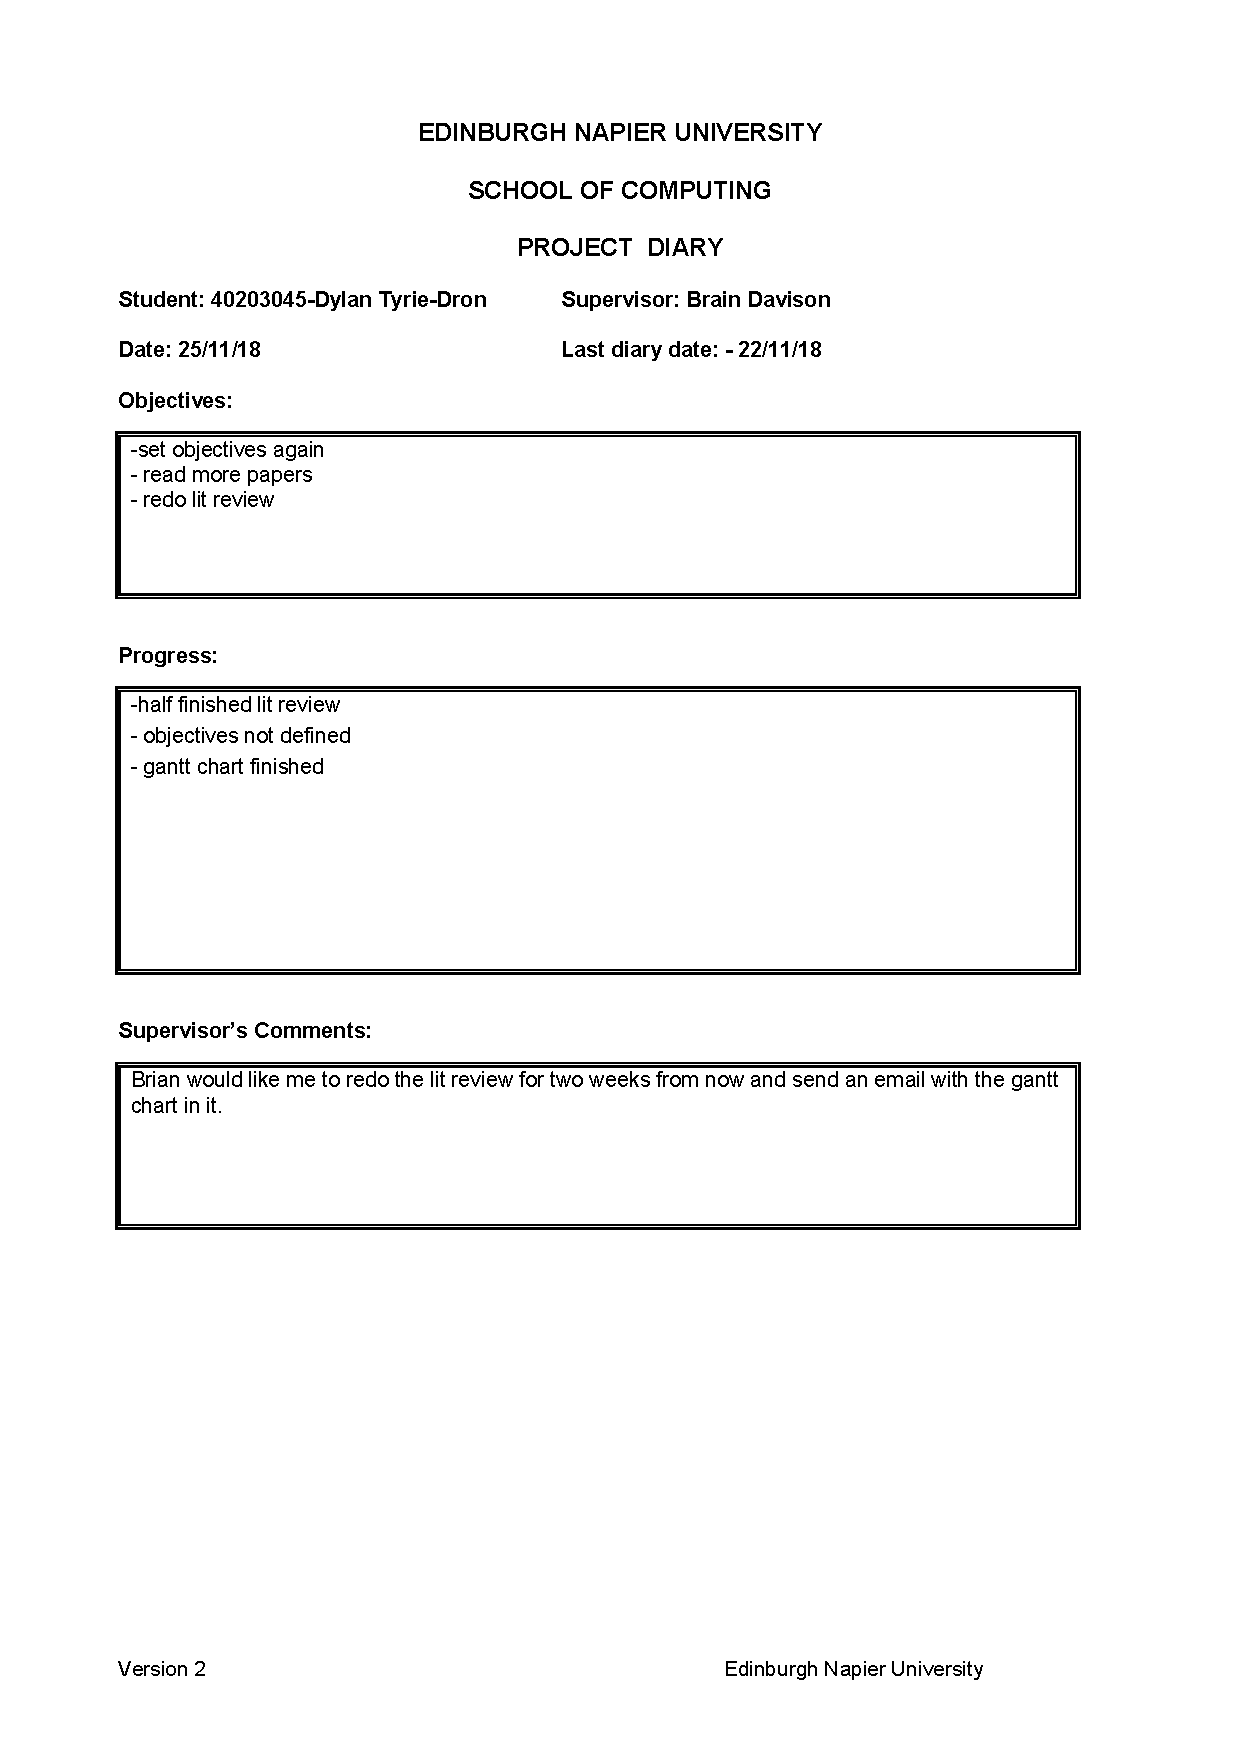
\includegraphics[width=\textwidth,height=\textheight,keepaspectratio]{project_diary_8th_entry.pdf}
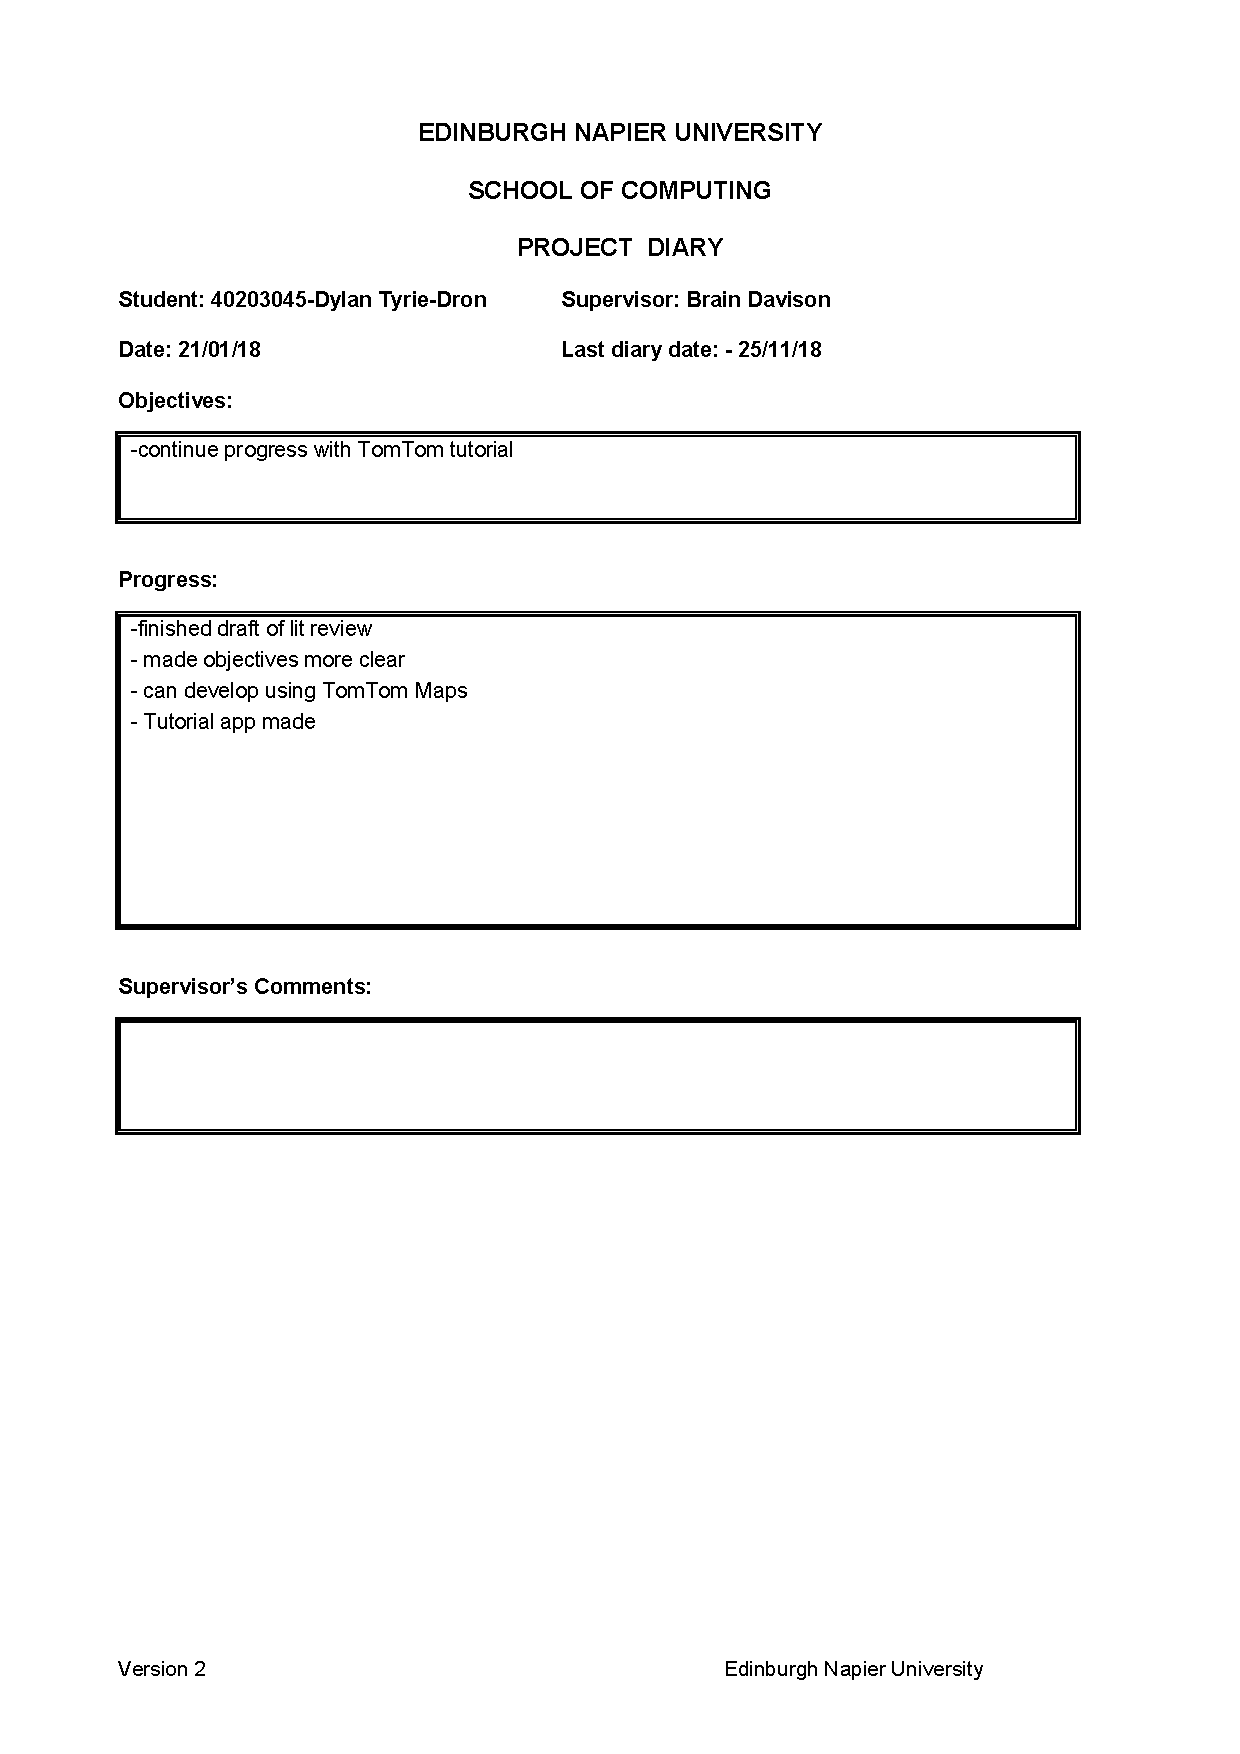
\includegraphics[width=\textwidth,height=\textheight,keepaspectratio]{project_diary_9th_entry.pdf}
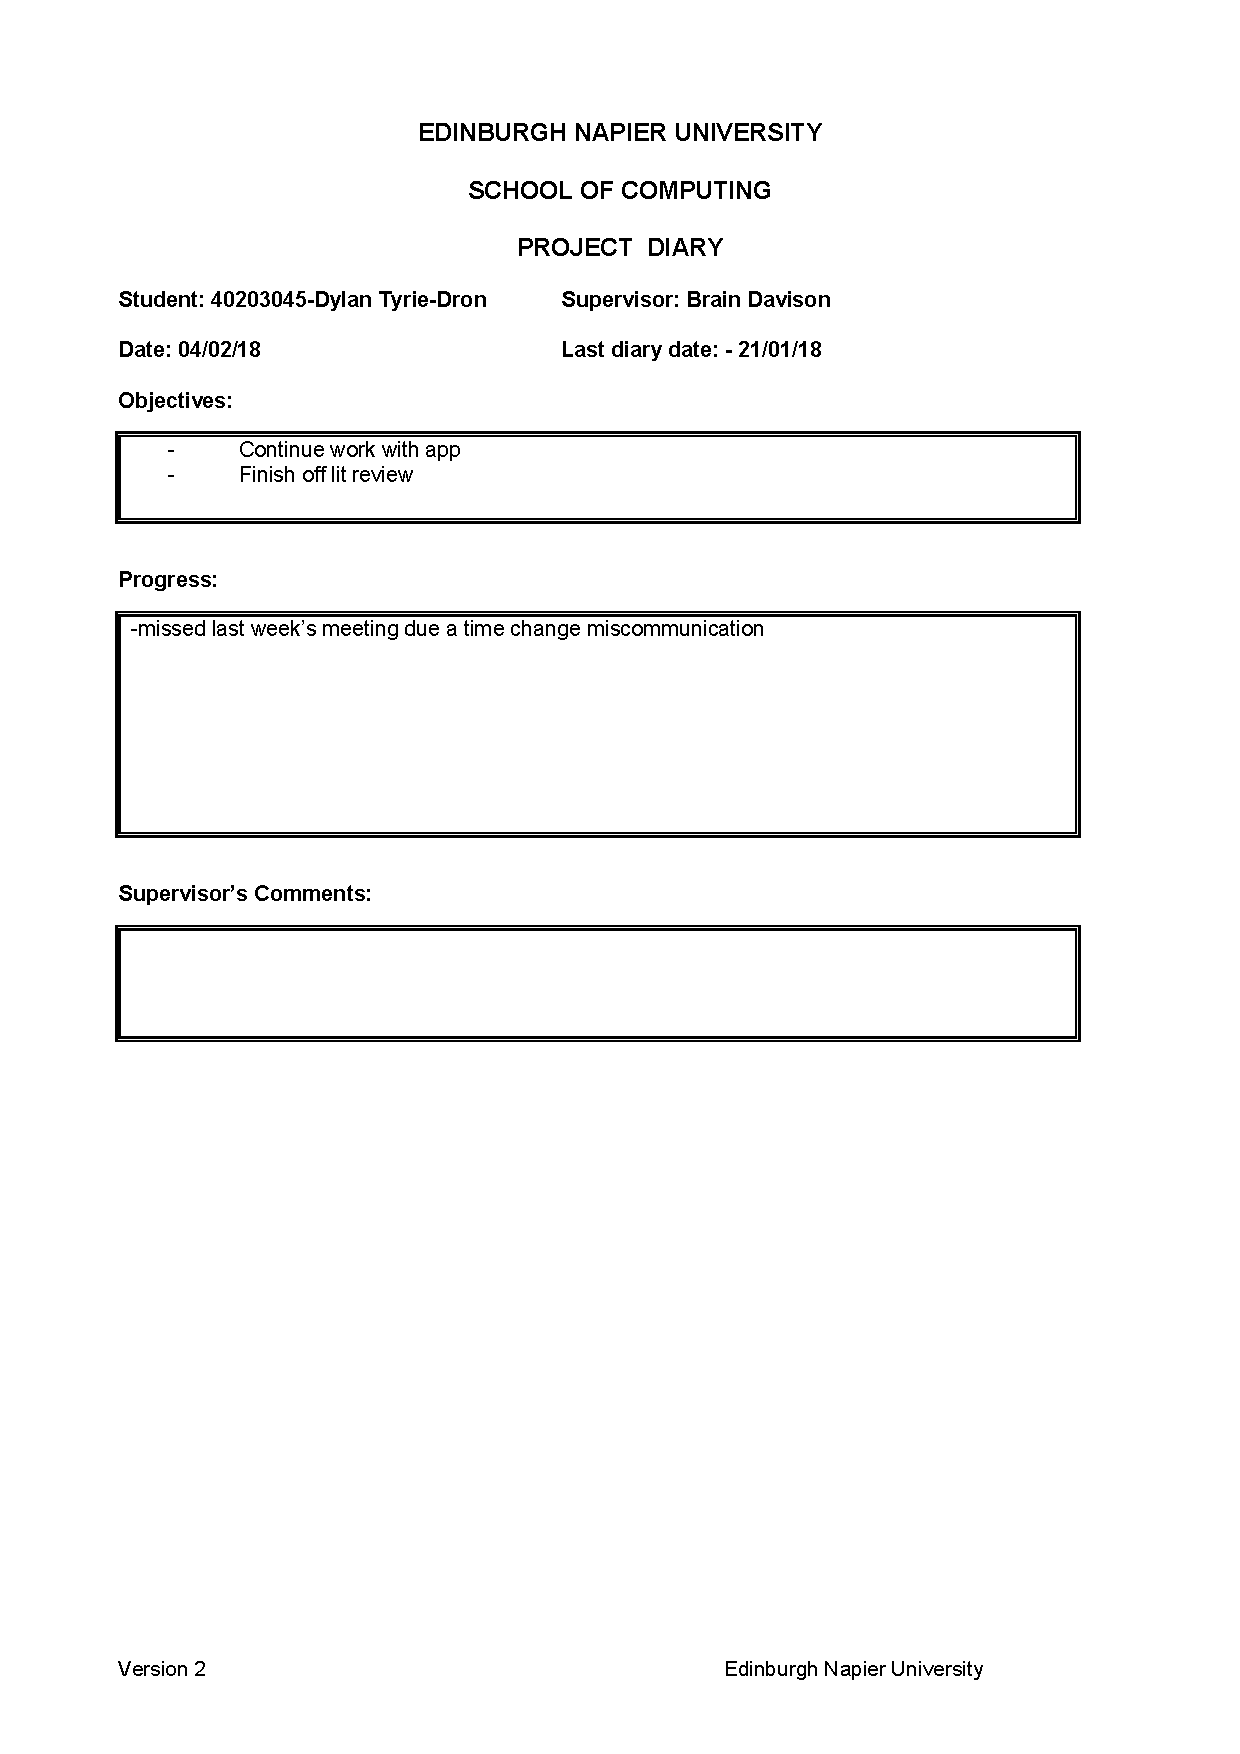
\includegraphics[width=\textwidth,height=\textheight,keepaspectratio]{project_diary_10th_entry.pdf}
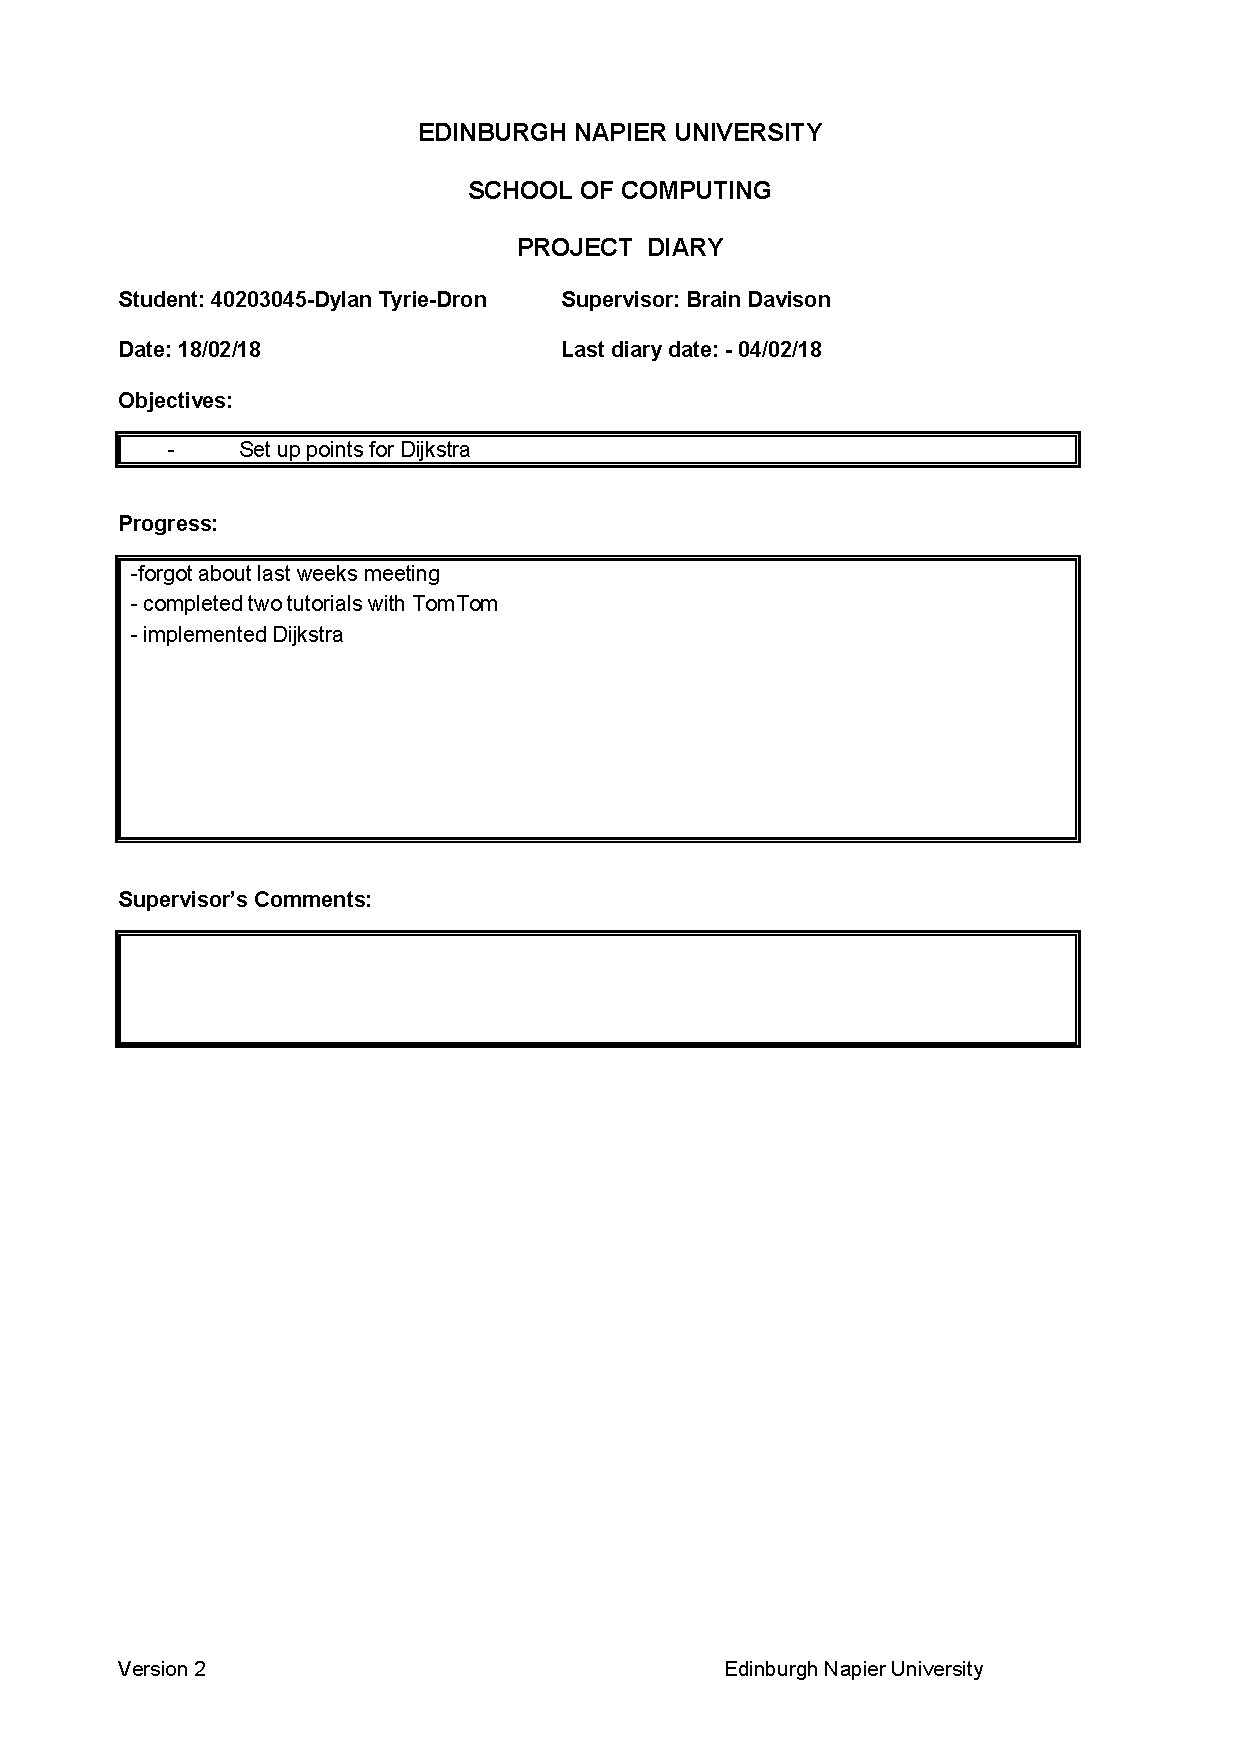
\includegraphics[width=\textwidth,height=\textheight,keepaspectratio]{project_diary_11th_entry.pdf}
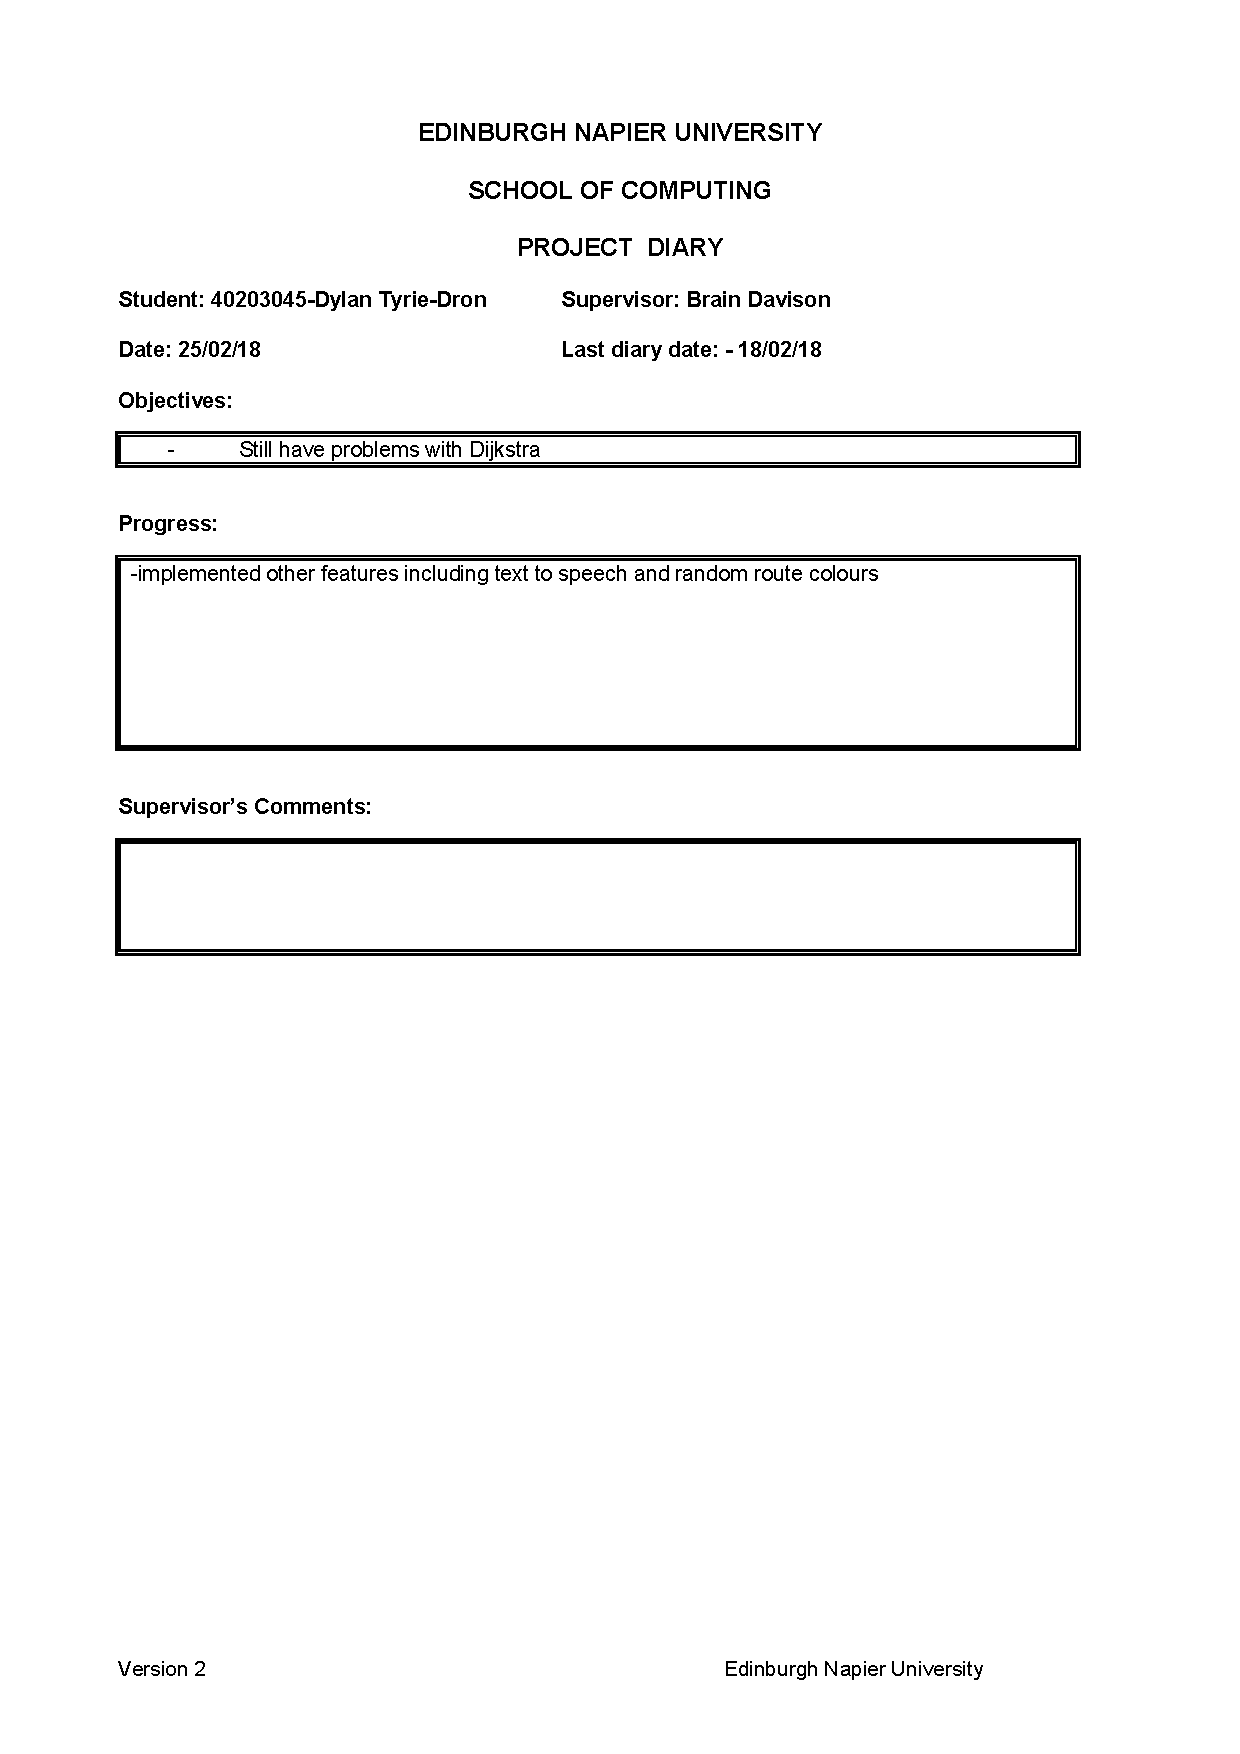
\includegraphics[width=\textwidth,height=\textheight,keepaspectratio]{project_diary_12th_entry.pdf}
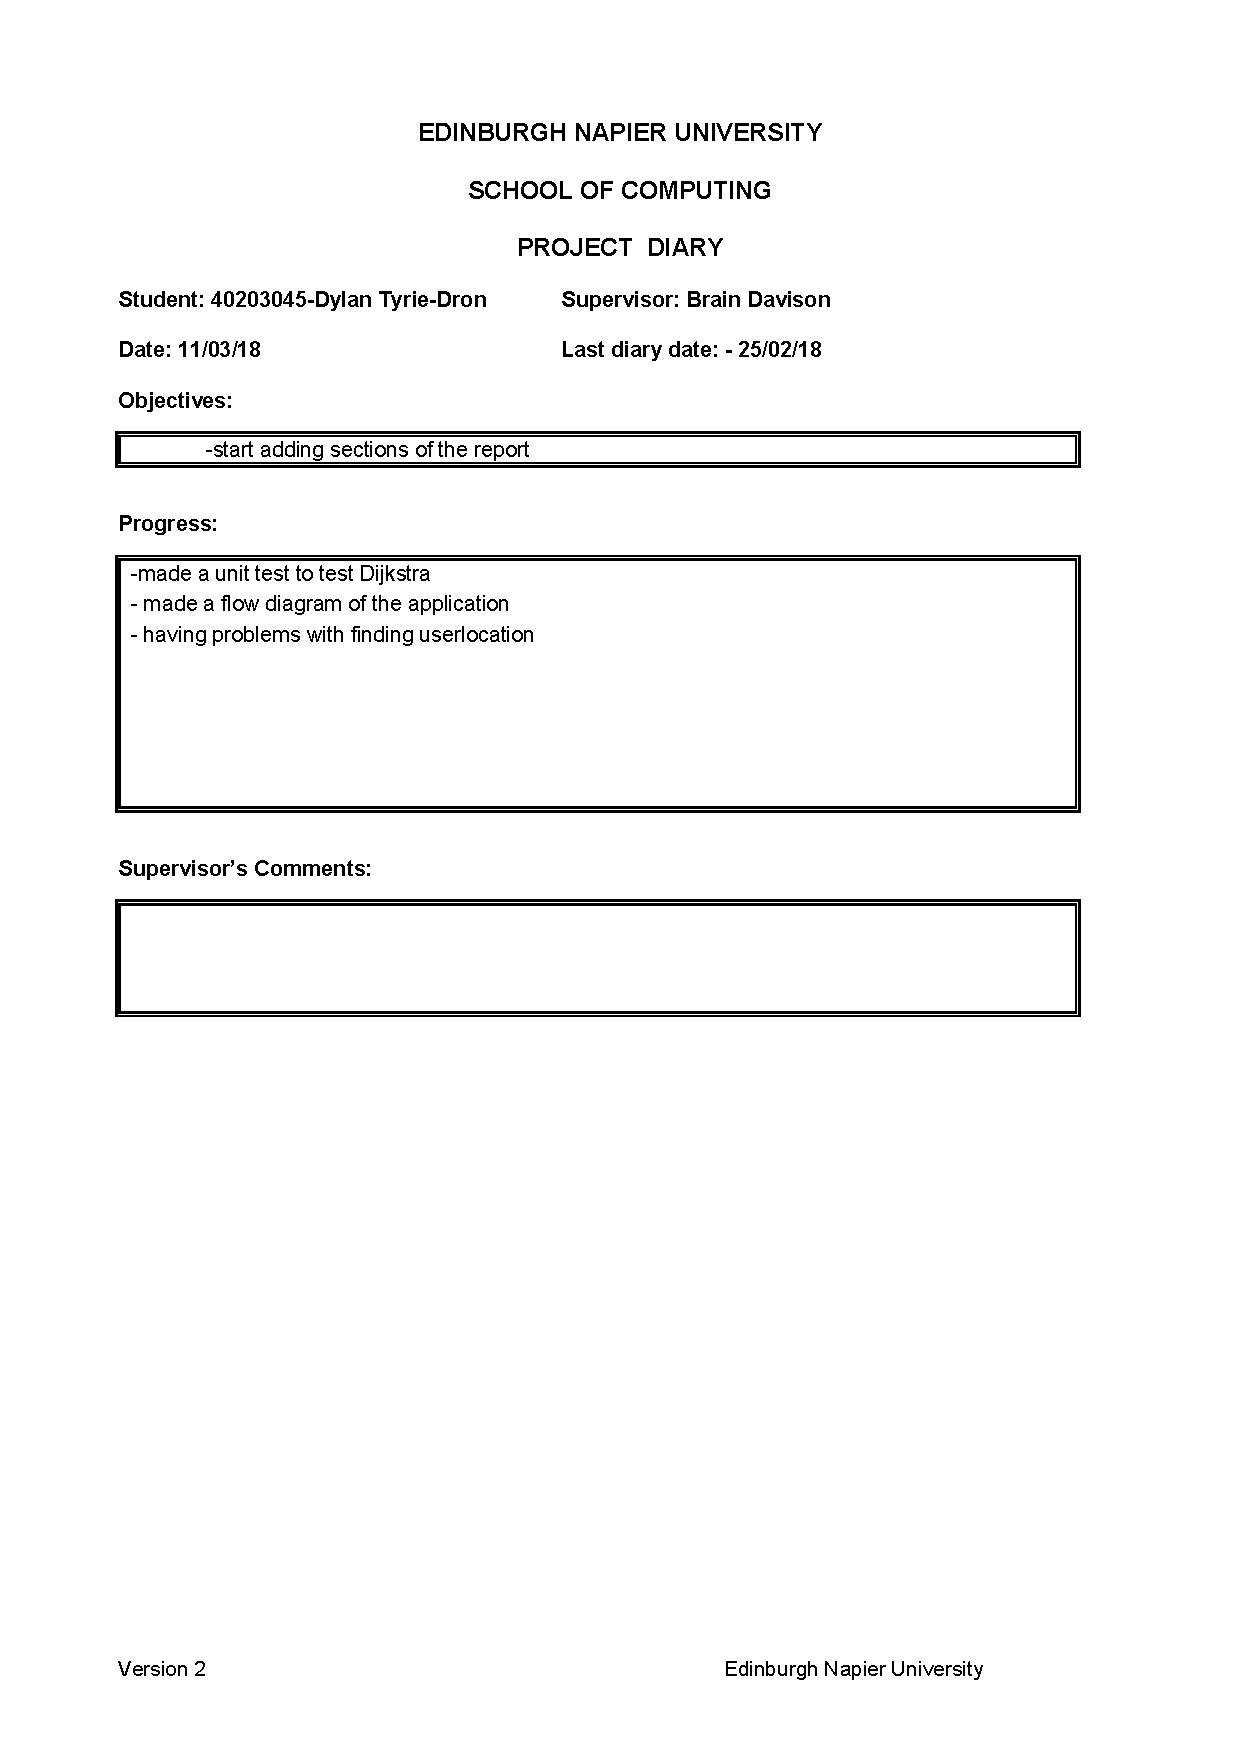
\includegraphics[width=\textwidth,height=\textheight,keepaspectratio]{project_diary_13th_entry.pdf}
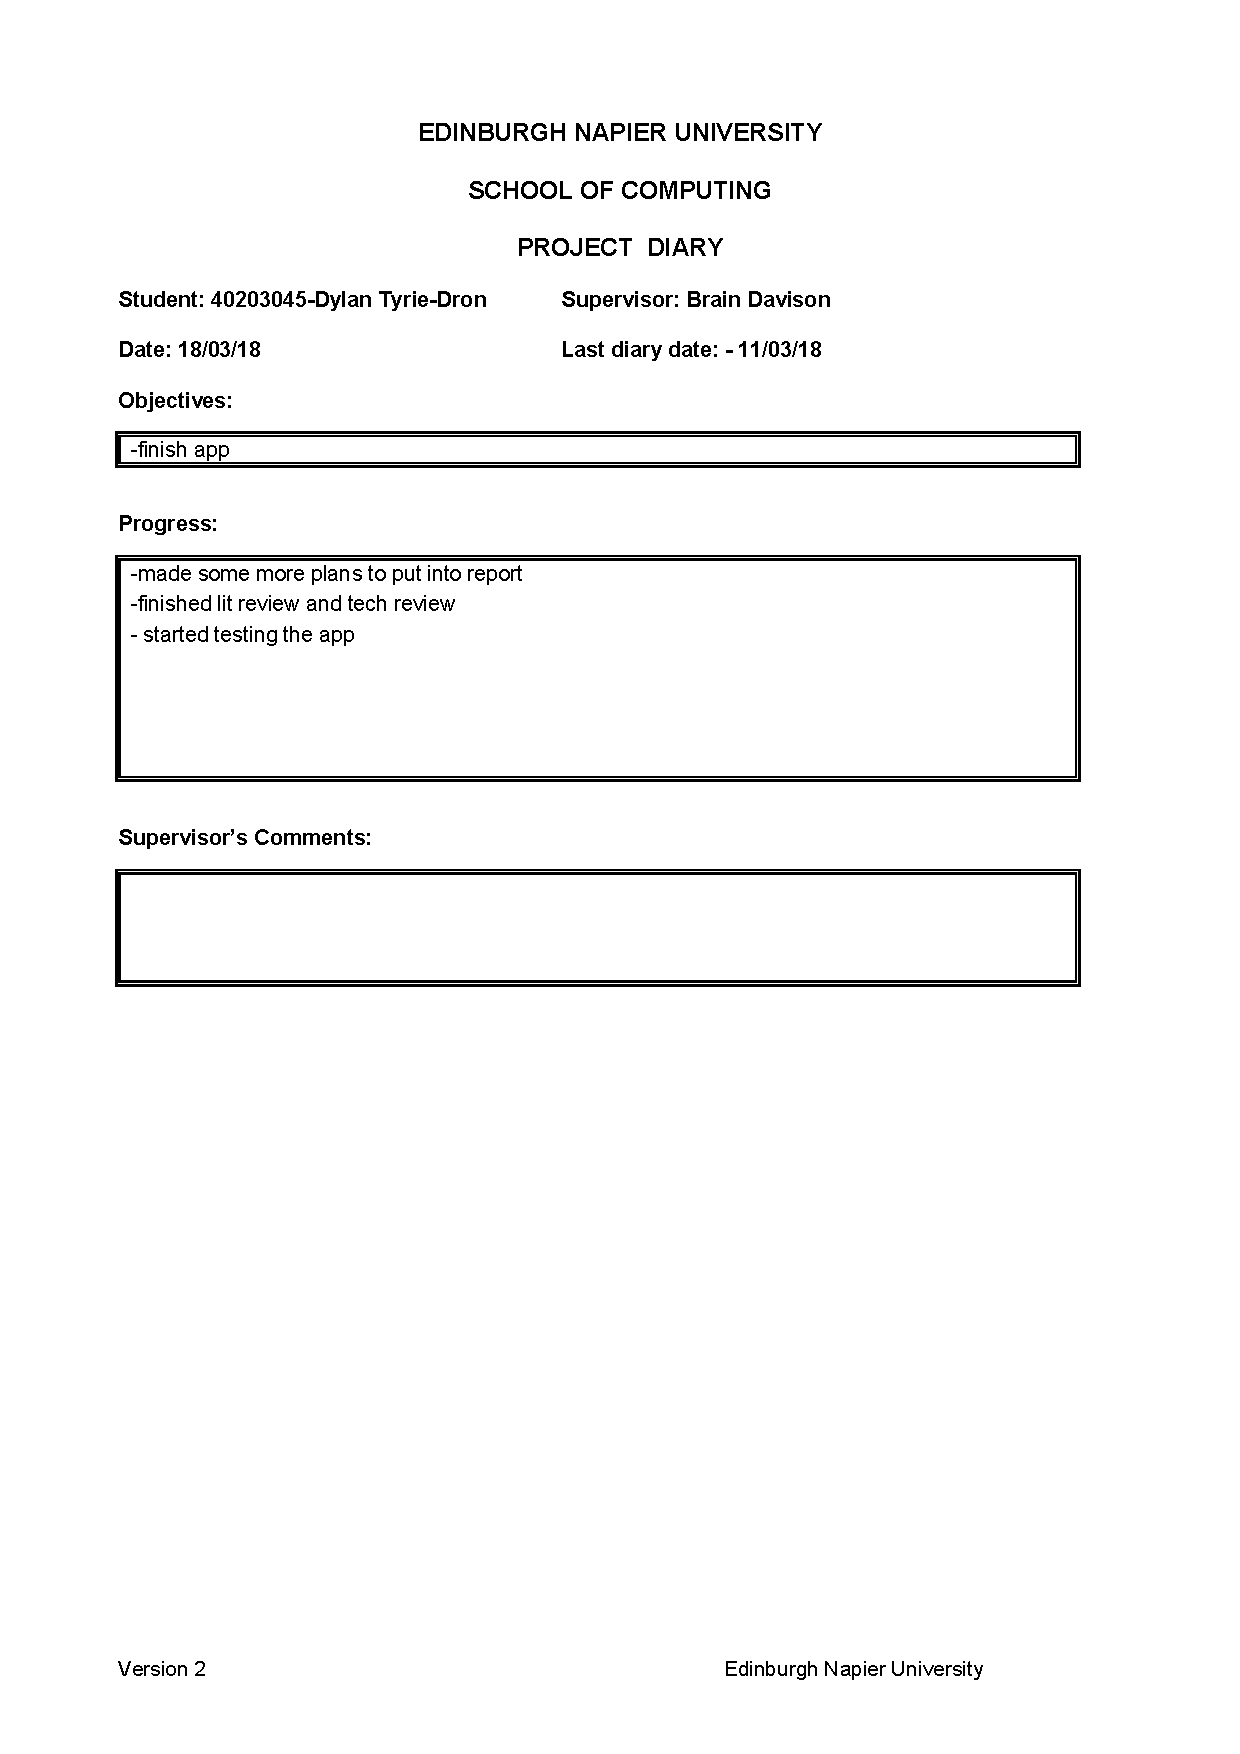
\includegraphics[width=\textwidth,height=\textheight,keepaspectratio]{project_diary_14th_entry.pdf}
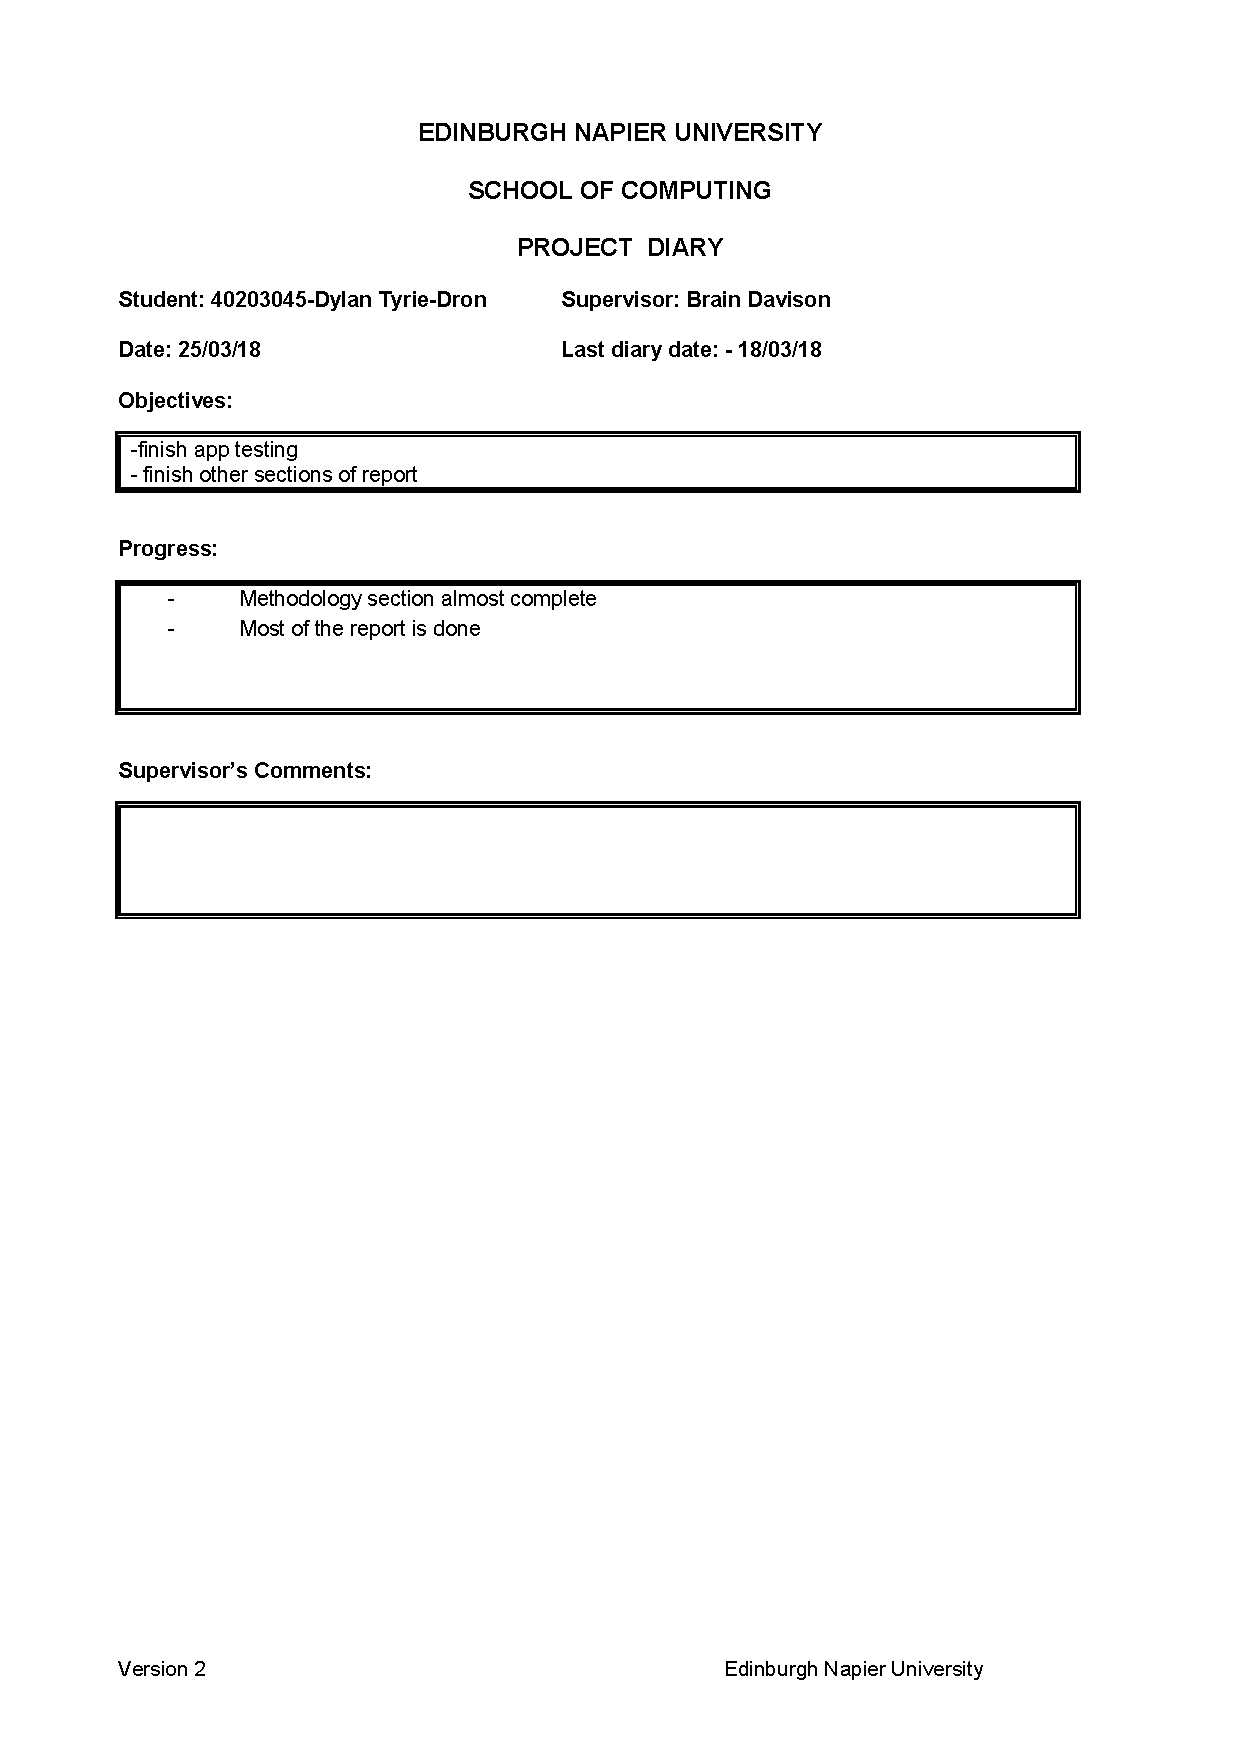
\includegraphics[width=\textwidth,height=\textheight,keepaspectratio]{project_diary_15th_entry.pdf}

\section{MoSCoW Method}
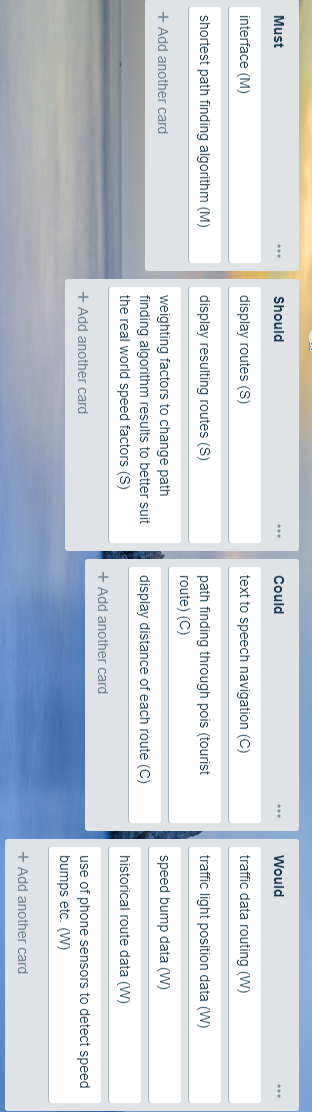
\includegraphics[width=\textwidth,height=\textheight,keepaspectratio]{MoSCoWMethod.png}
\section{Sprint Backlog}
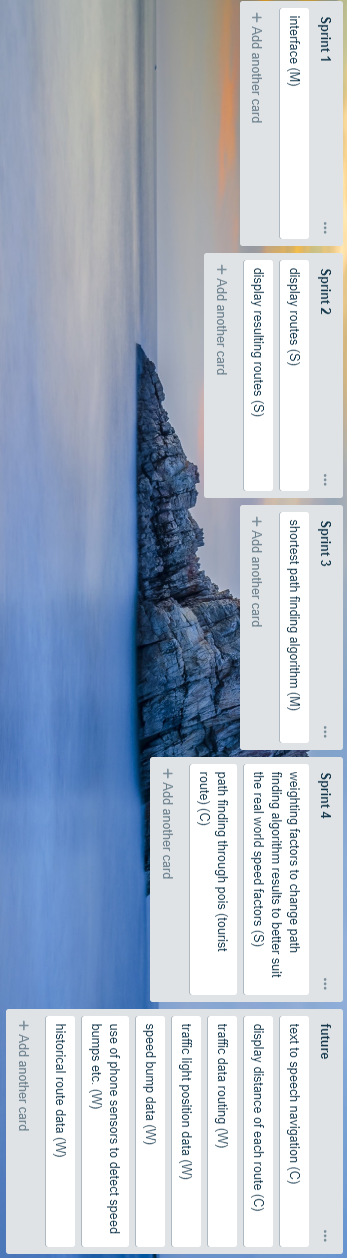
\includegraphics[width=\textwidth,height=\textheight,keepaspectratio]{sprintBacklog.png}
\section{Project Flow Diagram}
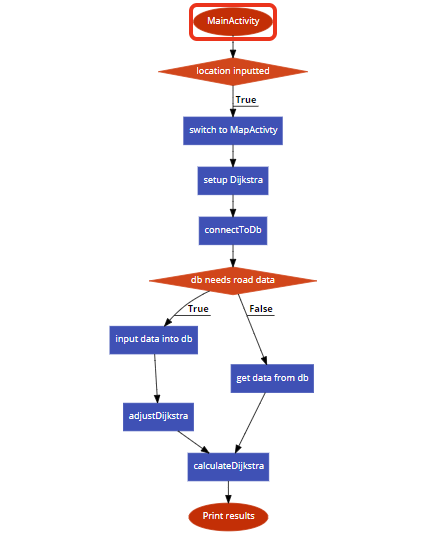
\includegraphics[width=\textwidth,height=\textheight,keepaspectratio]{flowDiagram.png}
\newpage

\section{Find edges for Dijkstra}
\lstinputlisting[basicstyle=\small, breaklines=true]{FindEdgesForDijkstra.java}
% \section{Appendix 4 and following}
% insert content here and for each of the other appendices, the title may be just on a page by itself, the pages of the appendices are not numbered, unless an included document such as a user manual or design document is itself pager numbered.
 \end{appendices}

\end{document}
